\chapter{Foundations of Deep Learning}
\label{ch:SNN}
Deep learning is a subfield of machine learning that leverages neural networks to model and solve complex problems. These neural networks are inspired by the structure and function of the human brain. A biological neuron consists of a cell body, dendrites, and an axon (Ref: Figure \ref{fig:neurons}). Dendrites receive signals from other neurons, which are processed in the cell body. Axons transmit electrical impulses to communicate information throughout the nervous system.

Similarly, artificial neural networks consist of interconnected nodes known as neurons, organized into layers. These artificial neurons, often referred to as perceptrons, receive input signals, process them, and produce an output. This analogy between biological and artificial neurons serves as the foundation of neural network architecture, allowing for the modeling and solution of complex problems.

\vspace{1.5em}

\begin{figure}[h]%
\centering
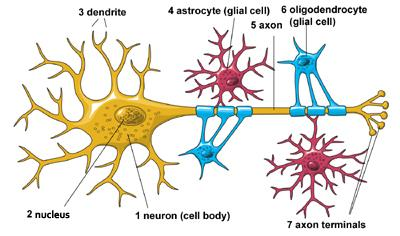
\includegraphics[width=0.65\textwidth]{imgs/NeuronArchitecture.jpg}
\caption{Neuron Architecture (Image taken from \href{https://www.ninds.nih.gov/}{National Institute of Neurological Disorders and Stroke, United States of America}, accessed on 20-May-2024).}\label{fig:neurons}
\end{figure}

\noindent Deep Learning Model များသည်  လူသားများ၏ အာရုံကြောစနစ်ရှိ neuron များ၏ အလုပ်လုပ်ပုံကို နမူနာယူ၍ တည်ဆောက်ထားခြင်းဖြစ်သည်။ neuron များသည် အချက်အလက်များကို ပို့ဆောင်ပေးခြင်း၊ သယ်ယူပေးခြင်းတာ၀န်ကို ထမ်းဆောင်သည့် messenger များဖြစ်ကြသည်။ 

neuron တစ်ခုတွင် ပြင်ပ (သို့မဟုတ်) အခြား neuron များမှ အချက်အလက် (signal) များကို ရယူမည့်  wire မျှင်များ (dendrites) ၊ ပြင်ပသို့ အချက်အလက်များ ပေးပို့မည့် Axon ဟု ခေါ်သည့် output wire များ နှင့် neuron ၏ အဓိက ခန္ဓာကိုယ် (cell body) ဟု အပိုင်း (၃) ပိုင်း ပါ၀င်သည် (Ref: Figure \ref{fig:neurons})။ dendrites မှတဆင့် ရလာသည့် အချက်အလက်များကို neuron ၏ အဓိက ခန္ဓာကိုယ် (cell body)မှ တွက်ချက်မှုများ ပြုလုပ်ပြီးနောက် ရလာသည့် ရလဒ်များကို Axon ဟု ခေါ်သည့် output wire များ မှ တဆင့် အခြား neuron များသို့ ပို့ပေးပါသည်။ထိုသို့ပေးပို့လာသည့် အချက်အလက် (signal) များကို အခြား neuron တစ်ခုမှ လက်ခံရယူပြီး အချက်အလက်များ ဆက်လက်ပို့ဆောင်ခြင်းများ ပြုလုပ်ကြပါသည်။ ထိုကဲ့သို့ neuron များ ချိတ်ဆက် အလုပ်လုပ်ခြင်းကို neural network ဟု ခေါ်ဆိုခြင်း ဖြစ်သည်။ 

လူသားများ၏ အာရုံကြောစနစ်ကို အခြေခံ၍ Artificial neural network architecture များကို Artificial neurons များစွာ ပါ၀င်သည့် layer များဖြင့် ချိတ်ဆက် ဖွဲ့စည်းထားသည်။ Layer တစ်ခုတွင် တစ်ခုထက်ပိုသော neuron များ ပါ၀င်ပြီး အဆိုပါ neuron များမှ အချက်အလက်ရယူခြင်း၊ တွက်ချက်ခြင်းနှင့် ရလဒ်များထုတ်ပေးခြင်းတို့ကို ထမ်းဆောင်ကြသည်။ neural network architecture တစ်ခုတွင် input layer ၊  တစ်ခုထက်ပိုသော hidden layer များ နှင့် ရလဒ် ထုတ်ပေးသည့် output layer (neuron) တို့ ပါ၀င်သည်။ 

\section{Neural Network Architecture} \label{sec:architecture}

Deep learning models excel at tackling complex problems by leveraging neural networks with multiple hidden layers. However, to lay a solid foundation, we begin with one-layer neural networks before moving onto multi-layer neural networks. 

\subsection{Single-Layer Neural Network}\label{sec:SLP}
The simplest form of a neural network is the one-layer neural network, also known as a single-layer perceptron. This basic building block helps in understanding the more complex architectures used in deep learning. A one-layer neural network consists of three main components:

\begin{itemize}
  \item Input Layer: Takes input features.
  \item Weights and Bias: Each input is assigned a weight, and a bias term is added.
  \item Activation Function: Computes the output of the neuron.
\end{itemize}

Deep Learning Model များသည် hidden layer များစွာပါ၀င်သော neural network architecture များ ဖြစ်သည်။ သို့သော် neural network ၏ အခြေခံ သဘောတရားကို နားလည်စေရန်အတွက် layer တစ်ခုသာ ပါ၀င်သော  one-layer neural network  မှ စ၍ ရှင်းပြသွားမည် ဖြစ်သည်။ One-layer neural network သည် အလွယ်ကူ အရိုးရှင်းဆုံးသော neural network တစ်ခု ဖြစ်ပြီး အစိတ်အပိုင်း (၃)ခု ပါ၀င်သည်။ 

\begin{itemize}
  \item Input Layer: Input layer တွင် ပါ၀င်သည့်  neuron တစ်ခုချင်းစီသည် Input feature တစ်ခုစီနှင့် တိုက်ရိုက်ချိတ်ဆက်ထားသည်။ 
  \item Weights and Bias: weight (မြှောက်ဖော်ကိန်း) များသည် Input feature တစ်ခုချင်းစီ၏ အရေးပါမှုကို ဆုံးဖြတ်ပေးသည်။ ထို့အပြင် Bias Unit တစ်ခုကိုလည်း ထည့်သွင်းစဥ်းစားရမည်။ 
  \item Activation Function: Activation Function သည် တွက်ချက်မှုများကို ပြုလုပ်ပြီး ရလဒ်ကို ရှာပေးမည့် Function ဖြစ်သည်။ 
\end{itemize}

\begin{figure}[h]%
\centering
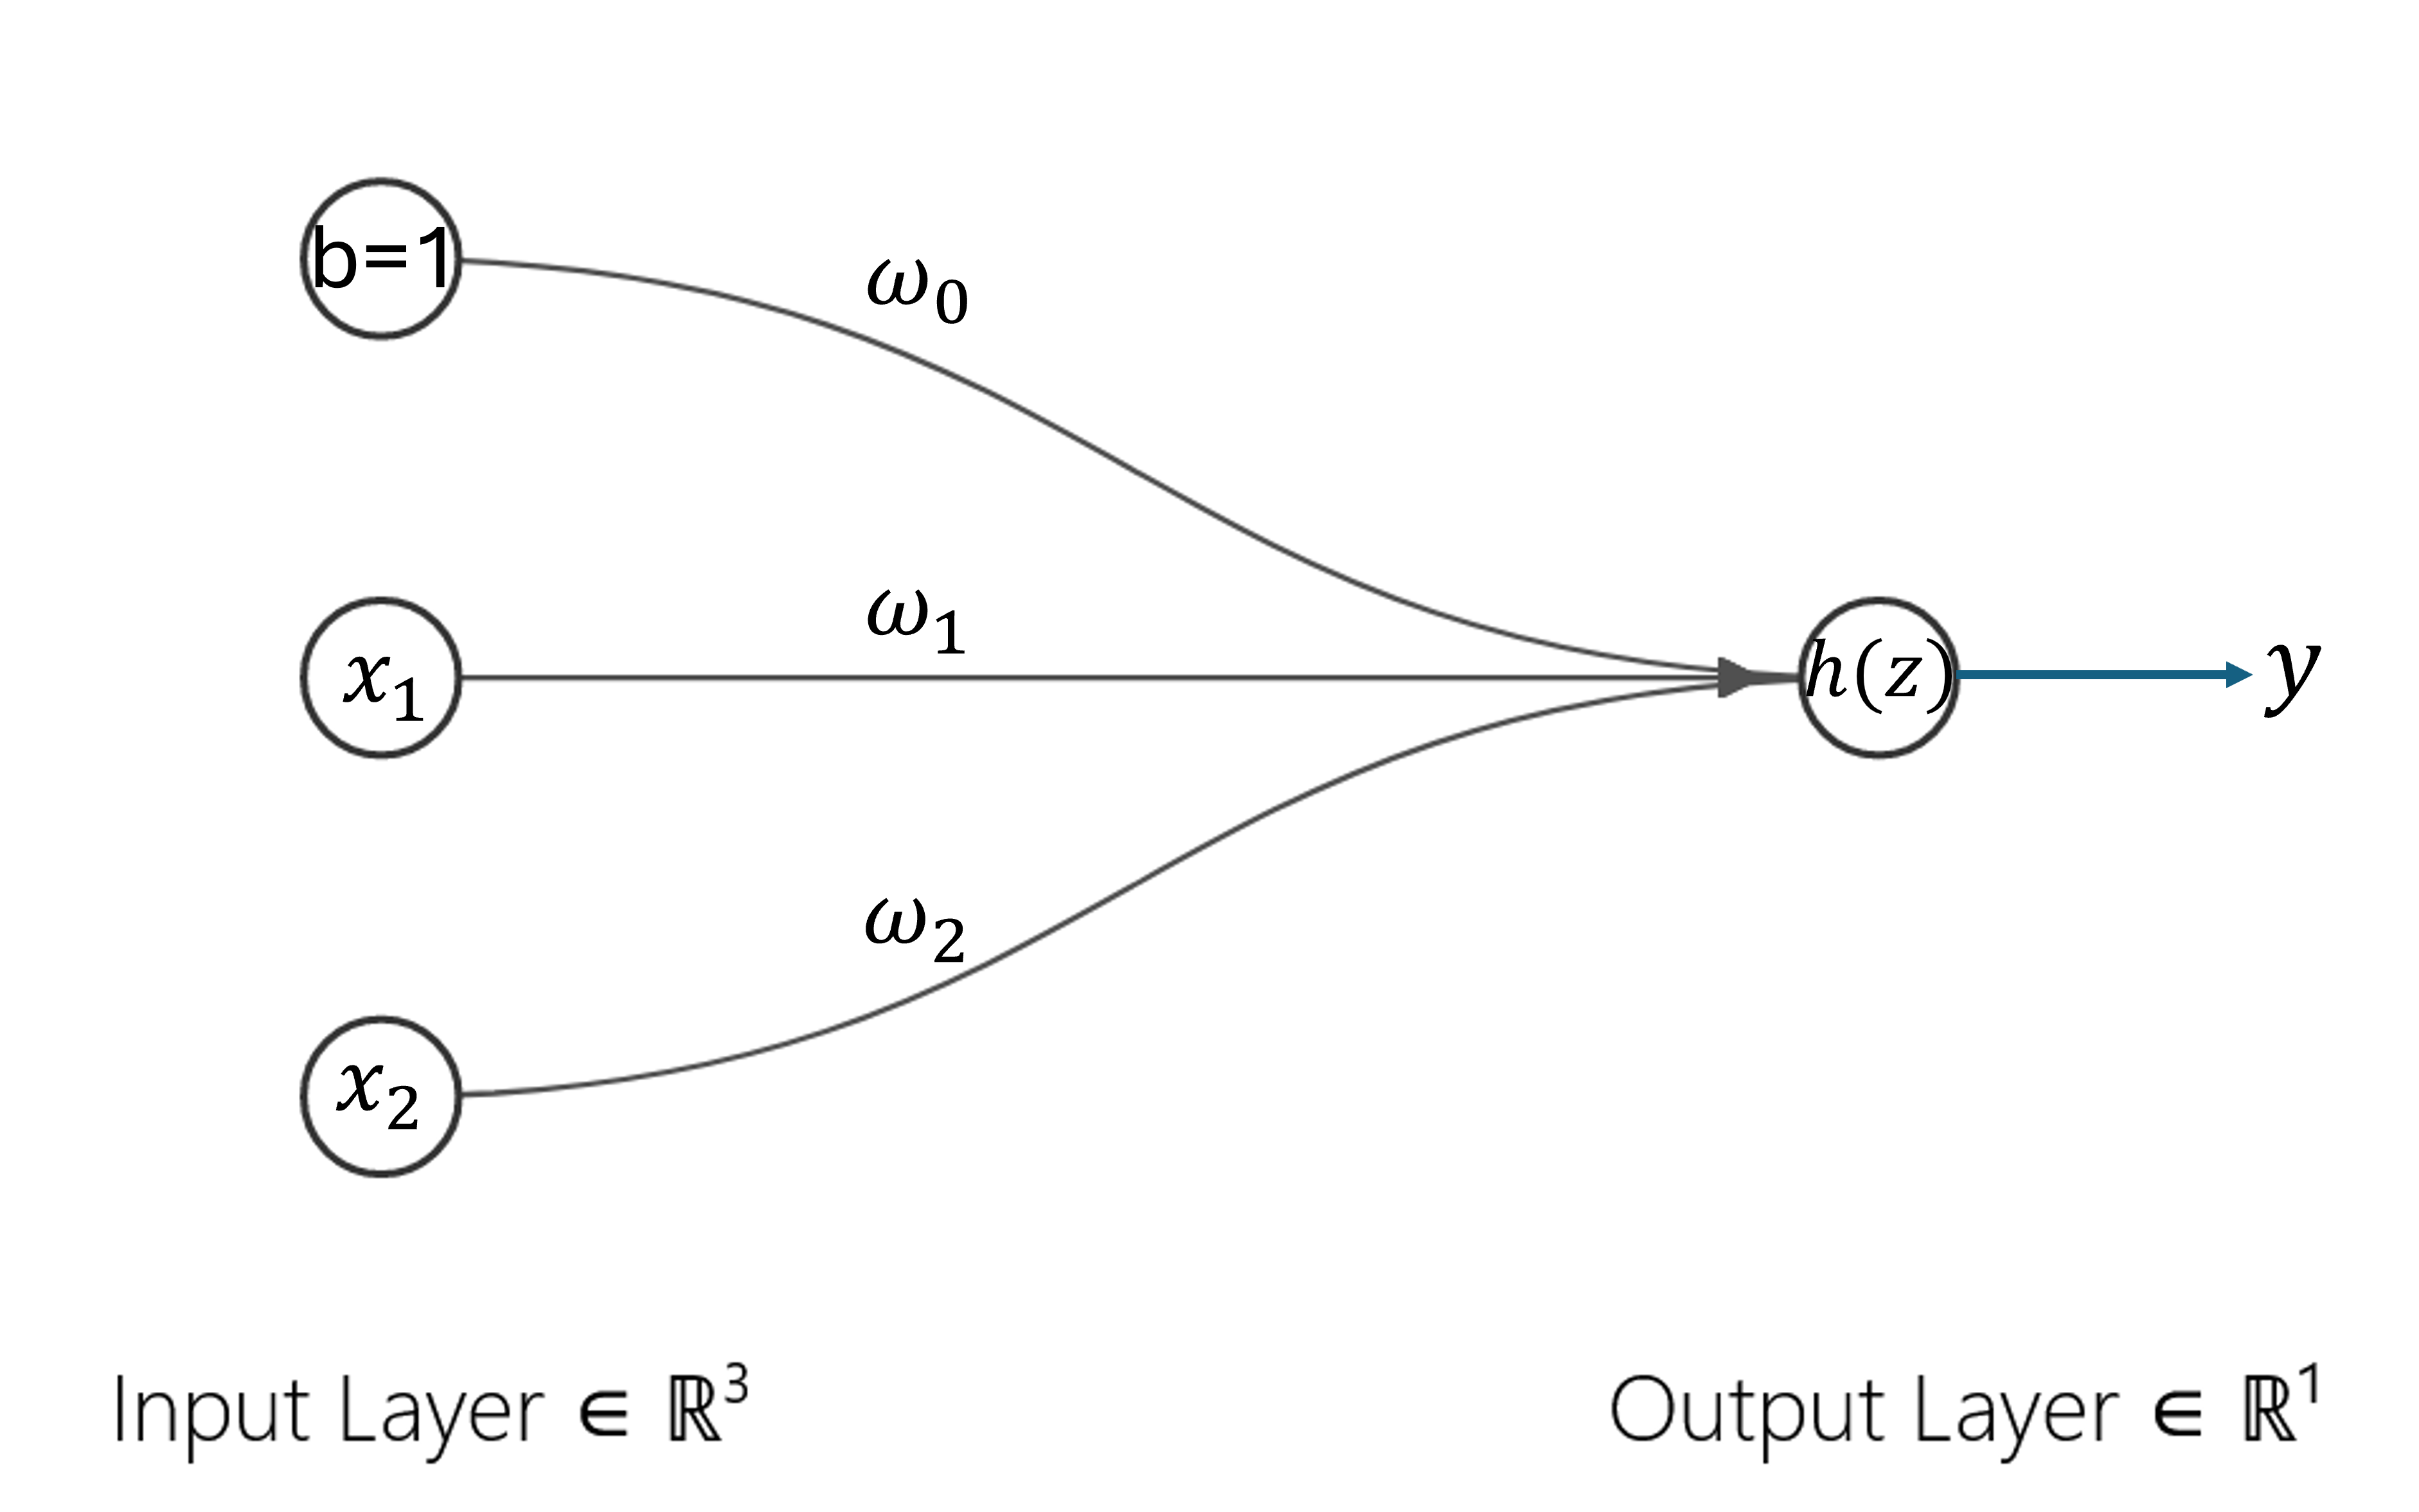
\includegraphics[width=0.675\textwidth]{imgs/slp.png}
\caption{Example of Single-Layer Perception (One Layer Neural Network) with two features. Image is generated using NN-SVG\cite{web:NNSVG}}\label{fig:slp}
\end{figure}

Figure \ref{fig:slp} illustrates a single-layer neural network with two input features. For example, suppose this network models the prediction of a company's sales amount based on TV and radio advertisement costs. The nodes $( x_1 ) $, $( x_2)$, represent these input features, while $( b = 1) $ serves as a bias unit. The bias unit $( b=1) $ is a constant added to the input to enhance model fitting. The weights $(\omega_1)$ and $(\omega_2)$ determine the importance of the associated features. The activation function $h(z)$ applies a transformation to the weighted sum of inputs and produces the output. During training, these weights are adjusted iteratively to minimize errors and ensure alignment between predicted and actual outputs.  

\noindent ဥပမာ - အထက်ပါပုံတွင် ပြသထားသည့် single-layer neural network သည် ကုမ္ပဏီတစ်ခု၏ ရောင်းအားကို ခန့်မှန်းပေးမည့် Machine Learning Model တစ်ခုဟု ဆိုကြပါစို့။  ကုမ္ပဏီ၏ ရောင်းအားကို TV နှင့် radio ကြော်ငြာခ အတွက် အသုံးပြုသည့် ကုန်ကျစရိတ်များကို မူတည်၍ ခန့်မှန်းမည်။ ဤဥပမာတွင် nodes $( x_1 ) $ နှင့် $( x_2)$ သည် TV နှင့် radio ကြော်ငြာခ များကို ကိုယ်စားပြုသည်။  

$( b = 1) $ သည် ကြော်ငြာခ လုံး၀ အသုံးမပြုသည့် အခြေအနေတွင် ဖြစ်ပေါ်နိုင်သည့် ရောင်းအားကို သိရှိနိုင်ရန် ထည့်ပေးသည့် ကိန်းသေတစ်ခုဖြစ်ပြီး bias unit ဟု ခေါ်သည်။ မြှောက်ဖော်ကိန်း $(\omega_1)$ နှင့် $(\omega_2)$ များသည် ရောင်းအားကို တွက်ချက်ရာတွင် TV နှင့် radio ကြော်ငြာခ တို့၏ အရေးပါမှုနှင့် တိုက်ရိုက်အချိုးကျသည်။ ဥပမာ - TV ကြော်ငြာခ တိုးလိုက်သည့် အချိန်တွင် ရရှိသည့် ရောင်းအား ပမာဏသည် radio ကြော်ငြာခ တိုးလိုက်သည့် အချိန်တွင် ရရှိသည့် ရောင်းအားပမာဏ ထက်များနေမည်ဆိုပါက $(\omega_1)$ ၏ တန်ဖိုးသည် $(\omega_2)$ ၏ တန်ဖိုးထက်များမည် ဖြစ်သည်။ 

Machine Learning Model တစ်ခုတည်ဆောက်သည် (သို့မဟုတ်) Train လုပ်သည် ဆိုသည်မှာ တနည်းအားဖြင့် အထက်ပါ မြှောက်ဖော်ကိန်း  $(\omega_1)$ နှင့် $(\omega_2)$ များ၏ တန်ဖိုးကို ရှာဖွေခြင်းပင် ဖြစ်သည်။ 

\subsection{Multi-layer Neural Network}\label{MLP}

A multi-layer neural network, specifically a Multi-Layer Perceptron (MLP), extends the concept of the single-layer perceptron by introducing one or more hidden layers between the input and output layers. This additional complexity allows the network to learn and represent more intricate patterns and relationships in the data, making it capable of solving more complex problems.

\noindent An MLP typically consists of three types of layers:
\begin{itemize}
  \item \textbf{Input Layer}: The layer that receives the input features.
  \item \textbf{Hidden Layers}: One or more intermediate layers where the computation happens. These layers perform transformations on the input data.
  \item \textbf{Output Layer}: The final layer that produces the output, such as class probabilities in classification tasks.
\end{itemize}

\begin{figure}[h]%
\centering
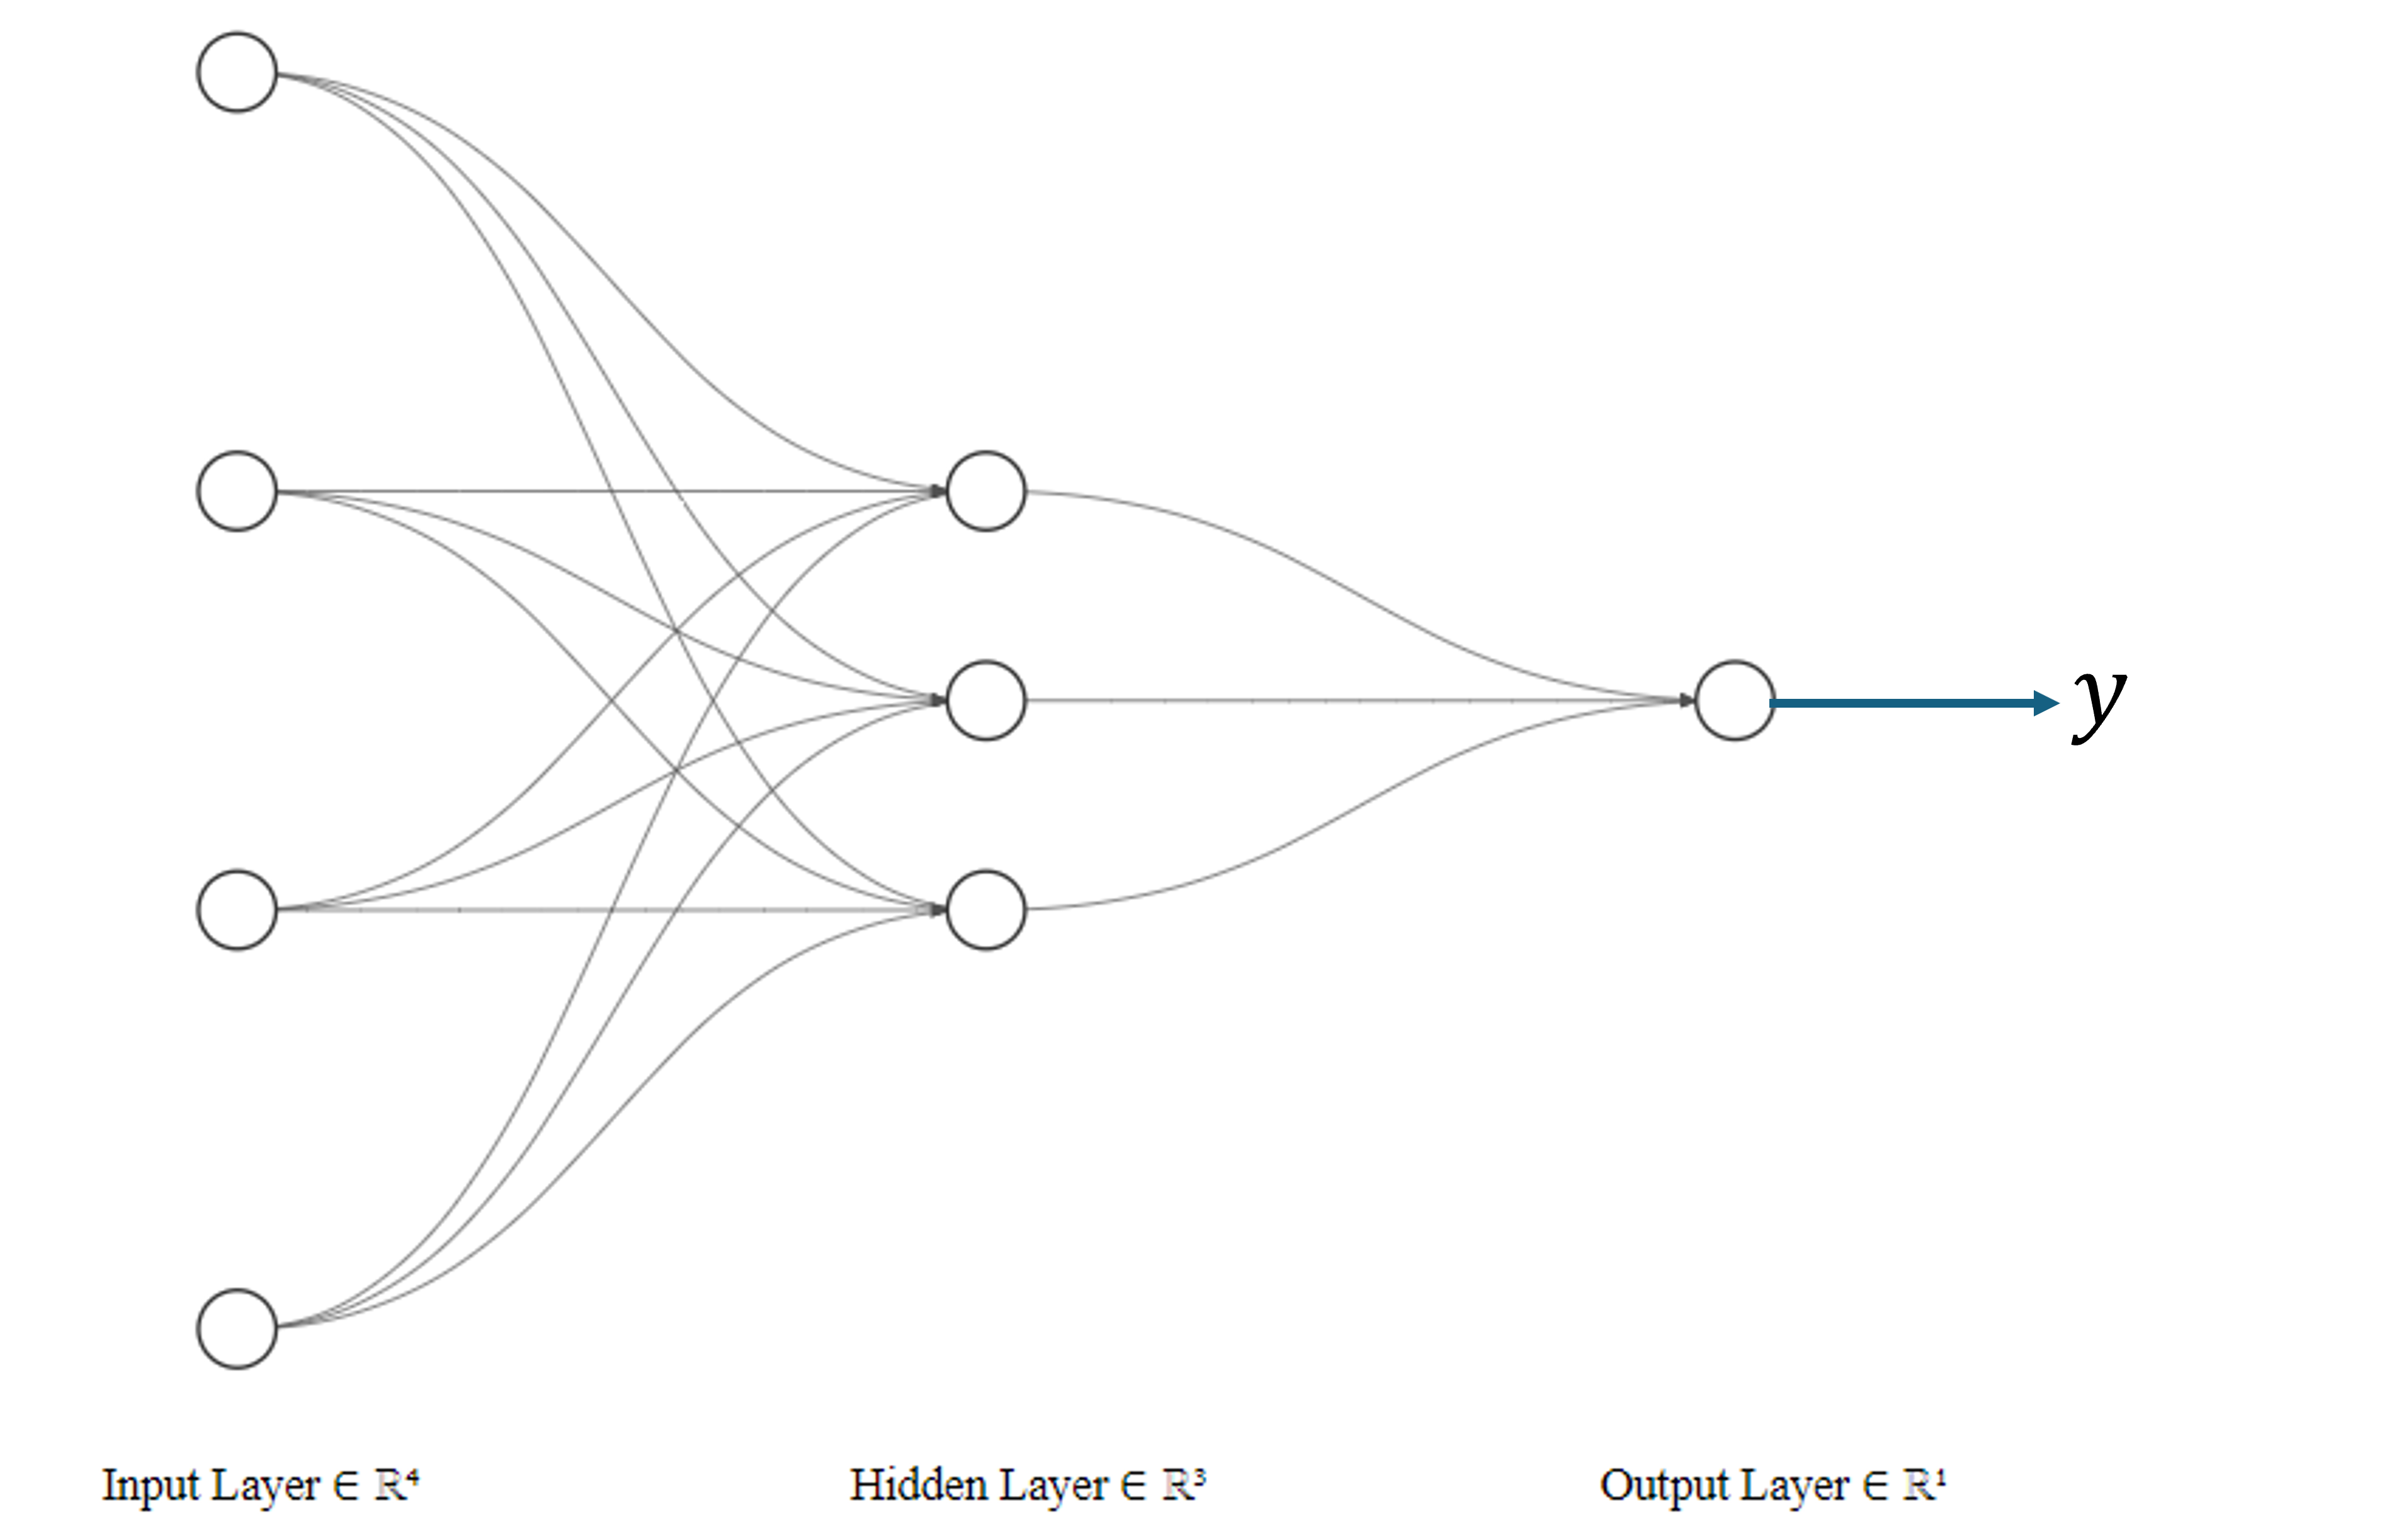
\includegraphics[width=0.7\textwidth]{imgs/mlp.png}
\caption{Example of Multi-Layer Perception with one hidden lyaer. Image is generated using NN-SVG\cite{web:NNSVG}}\label{fig:mlp}
\end{figure}

\vspace{0.25em}
\noindent Multi-layer neural network အထူးသဖြင့် Multi-Layer Perceptron သည်  single-layer perceptron (သို့) neural network တွင် hidden layer များထည့်ထားခြင်း ဖြစ်သည်။ Multi-Layer Perceptron တစ်ခုတွင် 

\begin{itemize}
  \item \textbf{Input Layer}: Input layer တွင် ပါ၀င်သည့်  neuron တစ်ခုချင်းစီသည် Input feature တစ်ခုစီနှင့် တိုက်ရိုက်ချိတ်ဆက်ထားသည်။ 
  \item \textbf{Hidden Layers}: ကြားခံ layer များဖြစ်ပြီး ၄င်း layer များသည် Input feature များကို အဆင့်ဆင့် ပြောင်းလဲ ပေးသွားသည်။ 
  \item \textbf{Output Layer}: Neural network ၏ နောက်ဆုံး layer ဖြစ်ပြီး output ကို ထုတ်ပေးသည်။ 
\end{itemize}

\subsection{Deep Learning Architecture}\label{deepNN}

The term \texttt{``deep learning"} refers to neural networks with multiple layers between the input and output layers \cite{Goodfellow-et-al-2016}. While traditional neural networks (often called shallow networks discussed in the previous chapter) typically have one or two hidden layers, deep learning networks usually have many more—sometimes reaching dozens or even hundreds of layers. This increased depth enables the network to learn hierarchical representations of data, capturing intricate features at various levels of abstraction \cite{lecun2015deep}.

A defining feature of deep learning is its ability to autonomously learn representations from raw data. Each subsequent layer in a deep network learns increasingly abstract features from the preceding one. For instance, when a deep neural network tries to classify an image, the initial hidden layers build up patterns or interactions that are conceptually simple. These initial layers look at groups of nearby pixels to find patterns like diagonal lines, horizontal lines, vertical lines, and areas of blur by examining groups of nearby pixels. As the network progresses through the layers, subsequent layers combine that information to detect larger patterns, such as squares or circles. Later layers put together these larger shapes to recognize complex structures like a checkerboard pattern, a face, or a car. 

The advantage of deep learning lies in its capacity to automatically acquire hierarchical features from data, facilitating precise identification and classification of objects in images. However, this prowess comes at a cost—deep networks necessitate substantial computational resources and large amounts of labeled data for effective training. Nonetheless, advancements in hardware, particularly Graphics Processing Units (GPUs), coupled with innovative algorithms, have rendered the training of these deep networks feasible.

Common deep learning architectures include Convolutional Neural Networks (CNNs) for image data, Recurrent Neural Networks (RNNs) and Long Short-Term Memory networks (LSTMs) for sequential data, and Transformer models for natural language processing. 

\vspace{0.5em}
\noindent Deep Learning သည် input နှင့် output layer အကြား layer များစွာ ပါ၀င်သည့် neural network model များ ဖြစ်သည်။ ပြီးခဲ့သည့် အခန်းတွင် ဆွေးနွေးခဲ့သည့် neural network model များတွင် hidden layer တစ်ခု (သို့မဟုတ်) နှစ်ခုသာ ပါ၀င်ကြပြီး ၄င်းတို့ကို \texttt{shallow} network များဟုလည်း ခေါ်ဆိုကြသည်။ Deep Learning model များတွင်မူ layer များစွာ ပါ၀င်ပြီး တစ်ခုနှင့် တစ်ခုအကြား ဒေတာများ၏ ချိတ်ဆက်မှုကို အဆင့်ဆင့် အလိုအလျောက် လေ့လာနိုင်သည်။ 

ဥပမာ - face image များကို အသုံးပြု၍  ဖုန်း authorize ပြုလုပ်မည့် deep learning model တစ်ခုတွင် Input Layer ၌ ပေးလိုက်သည့် ဒေတာများသည် image ရှိ pixel တစ်ခုချင်းစီ၏ intensity တန်ဖိုးများ ဆိုပါစို့။ အဆိုပါ  intensity များ၏ ချိတ်ဆက်မှုကို လေ့လာခြင်းဖြင့် ဒုတိယ Layer တွင် intensity တန်ဖိုးတူသည့် အုပ်စုများကို စုဖွဲ့ခြင်း၊ ရုတ်တရက် ပြောင်းလဲသွားသည့် pixel များကို ချိတ်ဆက်ခြင်းဖြင့် ဓါတ်ပုံတွင် ပါ၀င်သော မျက်နှာ၏ edge ကို detect လုပ်သွားနိုင်သည်။ ထိုမှတဆင့် အဆင့်ဆင့် Layer များတွင် မျက်နှာပြင်၏ ထူးခြားသည့် လက္ခဏာများကို ချိတ်ဆက် ပုံဖော်ခြင်းဖြင့် နောက်ဆုံးအဆင့်တွင် face image တွင် ပါ၀င်သည့် လူသည် authorize ပြုလုပ်သင့်သည့် ဟုတ်/မဟုတ်ကို မှန်မှန်ကန်ကန် ခန့်မှန်းနိုင်သည်။ 

\noindent သို့သော် ထိုကဲ့သို့ Layer များစွာ ပါ၀င်သည့် Deep Learning model တစ်ခုကို တည်ဆောက်နိုင်ရန်အတွက် အချက်အလက်များစွာ လိုအပ်သကဲ့သို့ computational power မြင့်မားသည့် ကွန်ပြူတာများ၊ ဆာဗာများလိုအပ်သည်။  GPU, or Graphics Processing Unit များထွက်ပေါ်လာခြင်းသည် Deep Learning model များ တည်ဆောက်ရန်အတွက် များစွာ အထောက်အကူ ဖြစ်စေသည်။ 

\noindent ယနေ့ခတ်တွင် လူသုံးများသည့် deep learning architecture များမှာ 
\begin{itemize}
  \item ဓါတ်ပုံ ၊ image ဒေတာများအတွက်  Convolutional Neural Networks (CNNs) ၊ 
  \item စာသား ၊ အသံစသည့် sequential ဒေတာများ အတွက် Recurrent Neural Networks (RNNs) နှင့် 
  \item Transformer model များဖြစ်ကြသည်။ 
\end{itemize}

\newpage 
\section{Activation Functions}\label{sec:activation}

The activation function $h(z)$ computes the final output of the neuron based on its pre-activation value. For a single neuron  in the neural network layer shown in Figure \ref{fig:slp}, the pre-activation value $z$ represents the weighted sum of inputs to a neuron, including the bias term.

\begin{equation}\label{eqn:hz}
  z = \omega_1 x_1 + \omega_2 x_2 + \omega_0, 
\end{equation} where 

\begin{itemize}[b]
  \item $(\omega_1)$ and $(\omega_2)$ are the weights associated with the connections from input features to the output neuron. 
  \item $( x_1 ) $, and $( x_2)$, are the input features (e.g., TV and radio advertisement costs).
  \item $b=1$ is the bias term associated with the output neuron.
\end{itemize}

\noindent In general, the equation \ref{eqn:hz} is written as: 
\begin{equation}\label{eqn:hz2}
  z = \sum_{i=1}^{n} \omega_i x_i + \omega_0, 
\end{equation} where $n$ is the number of features. 

\vspace{0.5em}
Common activation functions include Step, Sigmoid, ReLU (Rectified Linear Unit),  and Hyperbolic Tangent (tanh) Function. The choice of activation function depends on the specific task and the characteristics of the data. Experimentation with different activation functions is common to find the one that yields the best performance for a given problem.

\vspace{0.5em}
\noindent အထက်ပါပုံ  \ref{fig:slp} တွင် ပြသထားသည့် single-layer neural networkတွင် pre-activation value, $z$ ၏ တန်ဖိုးသည် မြှောက်ဖော်ကိန်းများနှင့် မြှောက်ထားသည့် ကြော်ငြာခ - ၂ ခု ၏ ပေါင်းခြင်းနှင့် ညီမျှသည် (ညီမျှခြင်း \ref{eqn:hz} ကို ကြည့်ပါ)။  ဤဥပမာတွင် input feature ၂ ခုသာပါ၀င်ပြီး $( x_1 ) $ နှင့် $( x_2)$ သည် TV နှင့် radio ကြော်ငြာခ များကို ကိုယ်စားပြုသည်။ input feature များစွာ ပါ၀င်သော ပုစ္ဆာအတွက် ဆိုပါက ညီမျှခြင်း \ref{eqn:hz2} ကို အသုံးပြုရမည်။ တနည်းဆိုသော် pre-activation value, $z$ သည် မြှောက်ဖော်ကိန်းများနှင့် မြှောက်ထားသည့် input feature များ၏ စုစုပေါင်းတန်ဖိုး ဖြစ်သည်။

\noindent Activation function အမျိုးမျိုးရှိပြီး လူသုံးများသည့် function များမှာ Step၊ Sigmoid၊  ReLU (Rectified Linear Unit) နှင့် Hyperbolic Tangent (tanh) Function တို့ဖြစ်ကြသည်။ ပုစ္ဆာ၏ သဘောတရားနှင့် ဒေတာ အမျိုးအစားများအပေါ်မူတည်၍ Activation function ကို ရွေးချယ်ကြလေ့ ရှိသည်။ 

\subsection{Step Function}\label{sec:activation}
This function produces binary output, typically 0 or 1, based on whether the input exceeds a certain threshold, $\theta$. It's commonly used for binary classification tasks. The mathematical representation of the step function, $h_{step}(z)$ is 
      \begin{equation}\label{eqn:step}
            h_{\text{step}}(z) = 
                                        \begin{cases}
                                        1, & \text{if } z \geq \theta \\
                                        0, & \text{otherwise}
                                        \end{cases}
    \end{equation} where $\theta$ is the threshold value. 
    
\begin{figure}[h]%
\centering
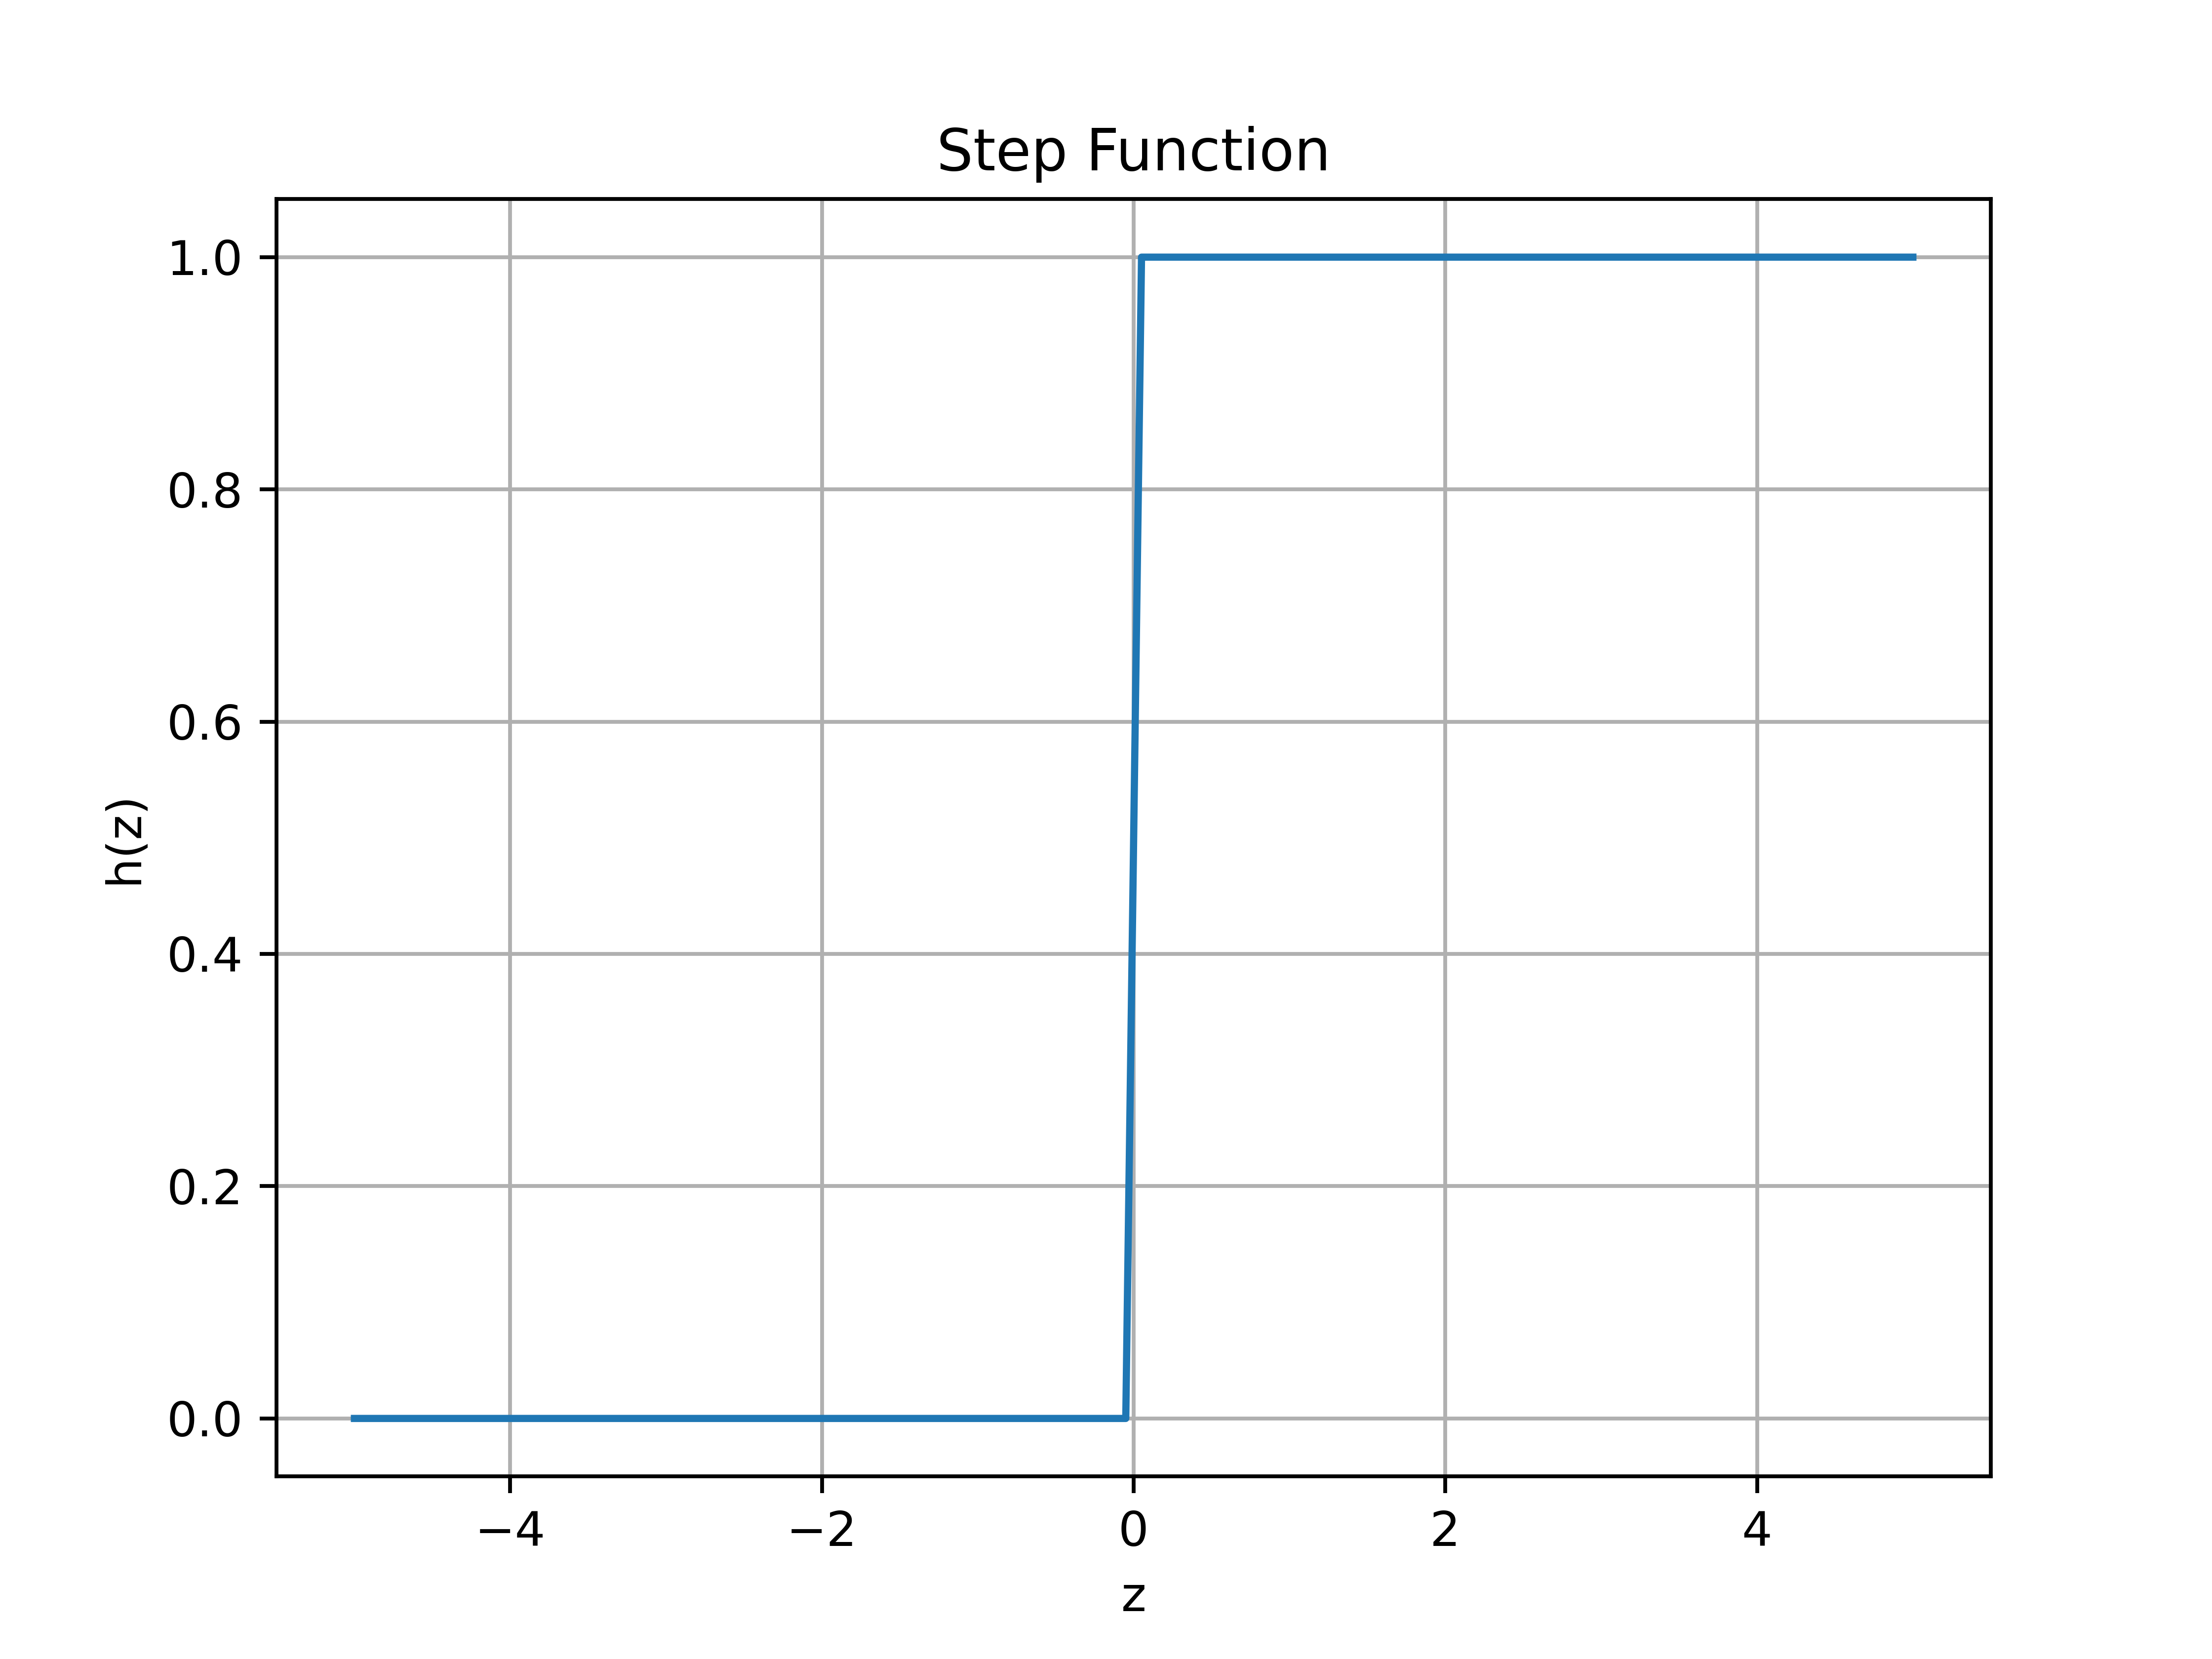
\includegraphics[width=0.6\textwidth]{imgs/step_fun.png}
\caption{Illustration of Step Function. Image is generated using Python.}\label{fig:step}
\end{figure}

Figure \ref{fig:step} illustrates a step function. As can be seen, the x-axis represents the pre-activation value $z$, and the y-axis represents the output of the function. It produces a binary value of 0 for all inputs below the threshold and 1 for all inputs above the threshold. The step activation function was historically used in early neural networks. However, it is rarely used in modern deep learning due to its binary nature.

\vspace{0.5em} 
Step Function ကို Binary classification ပုစ္ဆာများအတွက် အဓိက အသုံးပြုခဲ့ကြသည်။ Binary classification ပုစ္ဆာ နမူနာ အချို့မှာ - စာမေးပွဲ အအောင်၊ အရှုံး သတ်မှတ်ခြင်း၊ ပန်းသီး တစ်လုံး အပုတ်၊ အကောင်း ဆုံးဖြတ်ခြင်း စသည်တို့ ဖြစ်သည်။ ရလဒ်မှာ 'အောင်သည်' (သို့မဟုတ်) 'ကျသည်' - အဖြေ ၂ ခု အနက် - တစ်ခုသာ ဖြစ်သည်။ ပုံ  \ref{fig:step} တွင် Step Function ၏ သဘောတရားကို ဖော်ပြထားသည်။ အကယ်၍ pre-activation value $z$ ၏ တန်ဖိုးသည် ကြိုတင်သတ်မှတ်ထားသည့် ကိန်းသေ (threshold) ထက် နည်းပါက ရလဒ် - သုည (`ကျသည်') ကို ထုတ်ပေးပြီး ကိန်းသေ (threshold) ထက် များပါက ရလဒ် - တစ် (`အောင်သည်') ဟု ထုတ်ပေးမည် ဖြစ်သည်။ 

Step Function ကို ယနေ့ခတ်တွင် မသုံးသလောက် နည်းပါးသွားပြီဖြစ်သည်။ ဤ Function ၏ ပြဿနာမှာ ကိန်းသေ (threshold) ၏ နေရာတွင် သုညမှ တစ်သို့ ရုတ်တရက် ပြောင်းလဲသွားခြင်း ဖြစ်သည်။  ဥပမာ - စာမေးပွဲ အအောင် ၊ အရှုံး ပြဿနာတွင် - အောင်မှတ် (threshold) ကို ၄၀ ဟုတ် သတ်မှတ်ထားပါက ၄၀.၁ မှတ် ရသော ကျောင်းသားသည် အောင်သော်လည်း ၃၉.၉ မှတ်ရသော ကျောင်းသားသည် ကျမည် ဖြစ်သည်။ 

\subsection{Sigmoid Function}
The sigmoid function is often used in the output layer for problems where the output needs to be probabilistic or numerical. It squashes the input values to the range between 0 and 1, which can be interpreted as probabilities. For instance, in a binary classification problem, the output of the sigmoid function can represent the probability of belonging to one of the two classes. If the probability is above a certain threshold (e.g., 0.5), the input is classified into one class; otherwise, it's classified into the other class. Mathematically, it is represented as: 

\begin{equation}\label{eqn:sigmoid}
    h_{sigmoid}(z) = \frac{1}{1 + exp(-z)}
\end{equation} where pre-activation value, $z$ is the input to the function, typically the weighted sum of the inputs plus a bias term. 

\begin{figure}[h]%
\centering
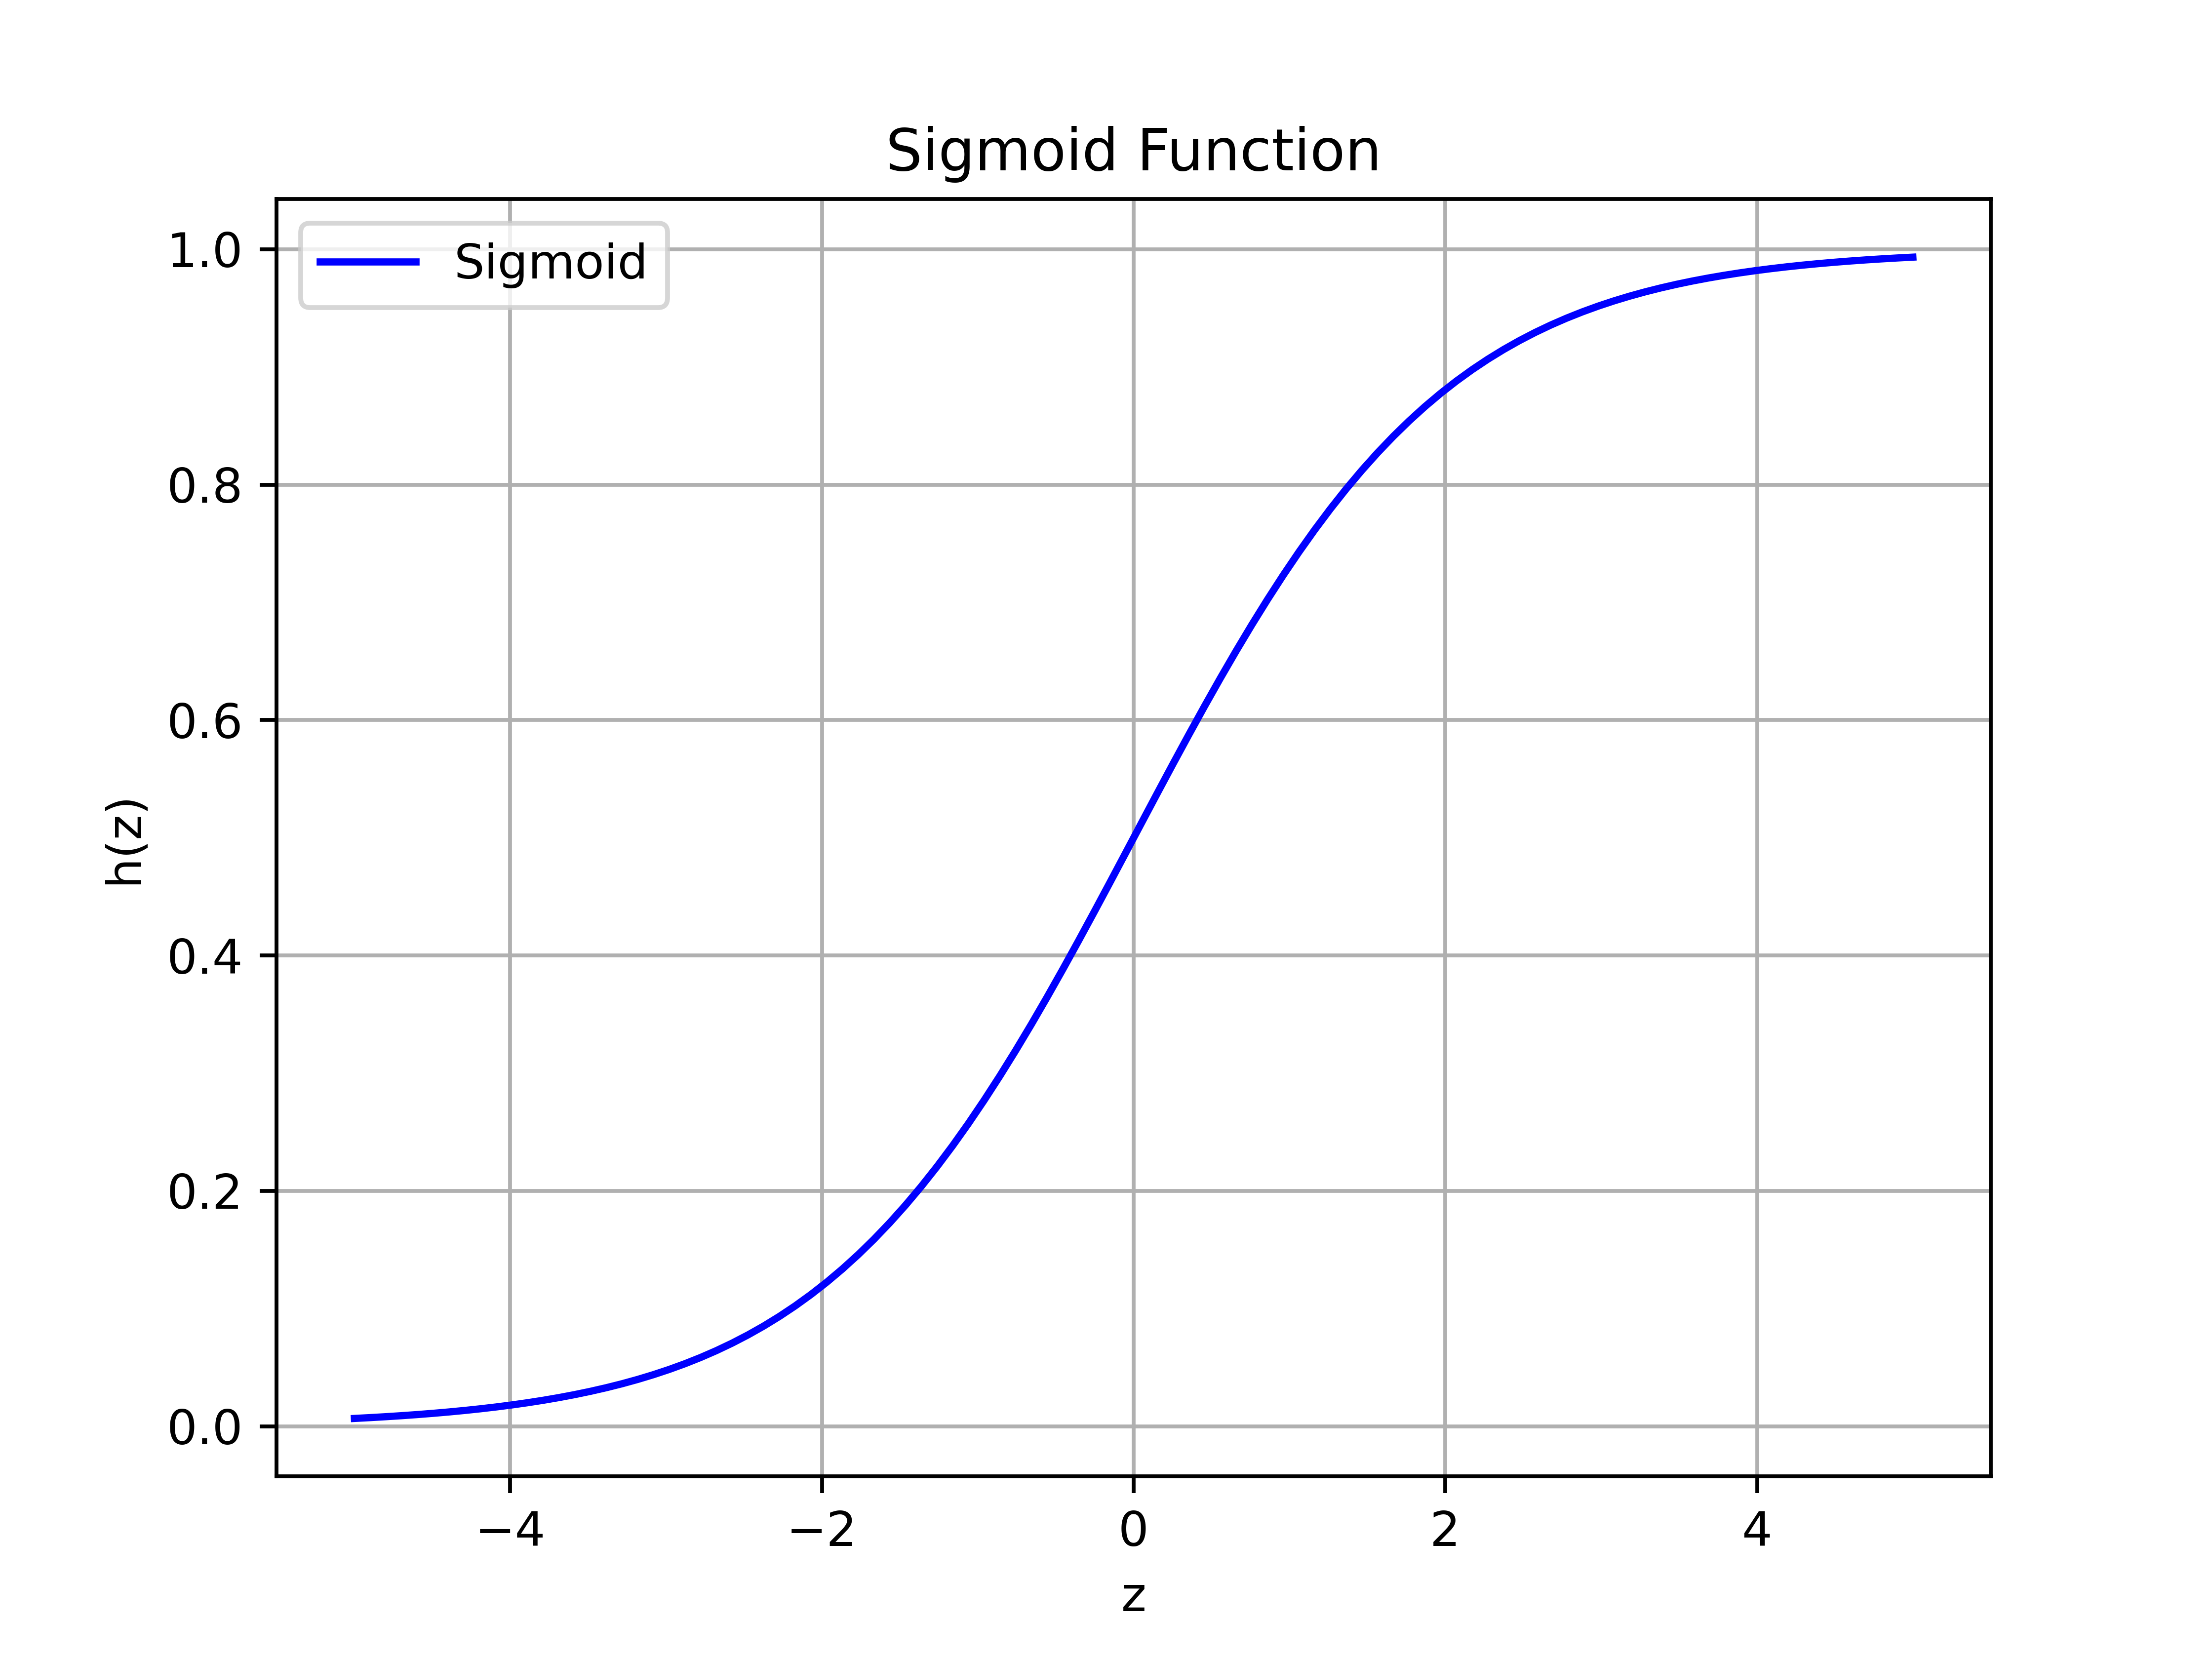
\includegraphics[width=0.55\textwidth]{imgs/sigmoid_fun.png}
\caption{Illustration of Sigmoid Function. Image is generated using Python.}\label{fig:sigmoid}
\end{figure}

As shown in Figure \ref{fig:sigmoid}, the sigmoid function is smooth and differentiable, which makes it suitable for gradient-based optimization techniques. However, one drawback is that it can cause the vanishing gradient problem in deep networks, where gradients become very small, slowing down or even preventing the network from training effectively. Despite this, the sigmoid function remains a popular choice for binary classification problems due to its probabilistic interpretation.

\vspace{1.5em} 

Sigmoid Function ကို Neural Network ၏ output layer အတွက် အသုံးပြုသည်။ ပုံ (\ref{fig:sigmoid}) တွင်ပြသထားသည့်အတိုင်း Sigmoid Function ၏ output သည် သုညမှ တစ် အတွင်းရှိပြီး probabilities တန်ဖိုးဟု ယူဆနိုင်သည်။ ဥပမာ - စာမေးပွဲ အအောင်၊ အရှုံး တွက်ချက်သည့် ပုစ္ဆာအတွက် Sigmoid Function သည် ကျောင်းသား၏ အောင်နိုင်ချေ ရာခိုင်နှုန်းကို တွက်ချက်ပေးသည်။ အကယ်၍ ကျောင်းသား (သို့မဟုတ်) ကျောင်းသူ ၏ pre-activation value $z$ သည် သုညထက်နည်းပါက Sigmoid Function ၏ တန်ဖိုးသည် ၀.၅ (သို့မဟုတ်) ၅၀ ရာခိုင်နှုန်းအောက် ဖြစ်မည် (ညီမျှခြင်း - \ref{eqn:sigmoid} ကို ကြည့်ပါ)။ 

ပုံ (\ref{fig:sigmoid}) တွင် မြင်ရသည့် အတိုင်း sigmoid function မှပေးသောရလဒ်သည် Step Function ကဲ့သို့ ရုတ်တရက် ပြောင်းလဲသွားခြင်းမျိုး မဟုတ်ဘဲ  ဖြည်းဖြည်းချင်း ပြောင်းလဲ သွားသည်။ pre-activation value $z$ ၏ တန်ဖိုအနည်း အများပေါ်မူတည်၍  sigmoid function ၏ ရလဒ်သည် သုည (သို့မဟုတ်) တစ် သို့ ဖြည်းဖြည်းချင်း ချဥ်းကပ်သွားသည်။ အဆိုပါ အားသာချက်ကြောင့် sigmoid function ကို Binary classification ပုစ္ဆာများအတွက် ယနေ့တိုင် အသုံးပြုနေဆဲ ဖြစ်သည်။ 

\subsection{Softmax Function} 

The Softmax function is an activation function commonly used in the output layer of neural networks for multi-class classification tasks. It transforms a vector of raw scores (logits) into a probability distribution, where each class's probability is proportional to the exponential of the logit for that class. The Softmax function ensures that the sum of the probabilities for all classes equals 1, making it possible to interpret the outputs as probabilities. The function is defined as:

\begin{equation}\label{eqn:softmax}
    h_{softmax}(z_i) = \frac{exp(z_i)}{\sum_{j=1}^{K}exp(z_j)}
\end{equation} where $z_i$ are the input logits for each class, $i$ and $K$ is the number of classes. 

\vspace{0.5em} 

\begin{figure}[h]%
\centering
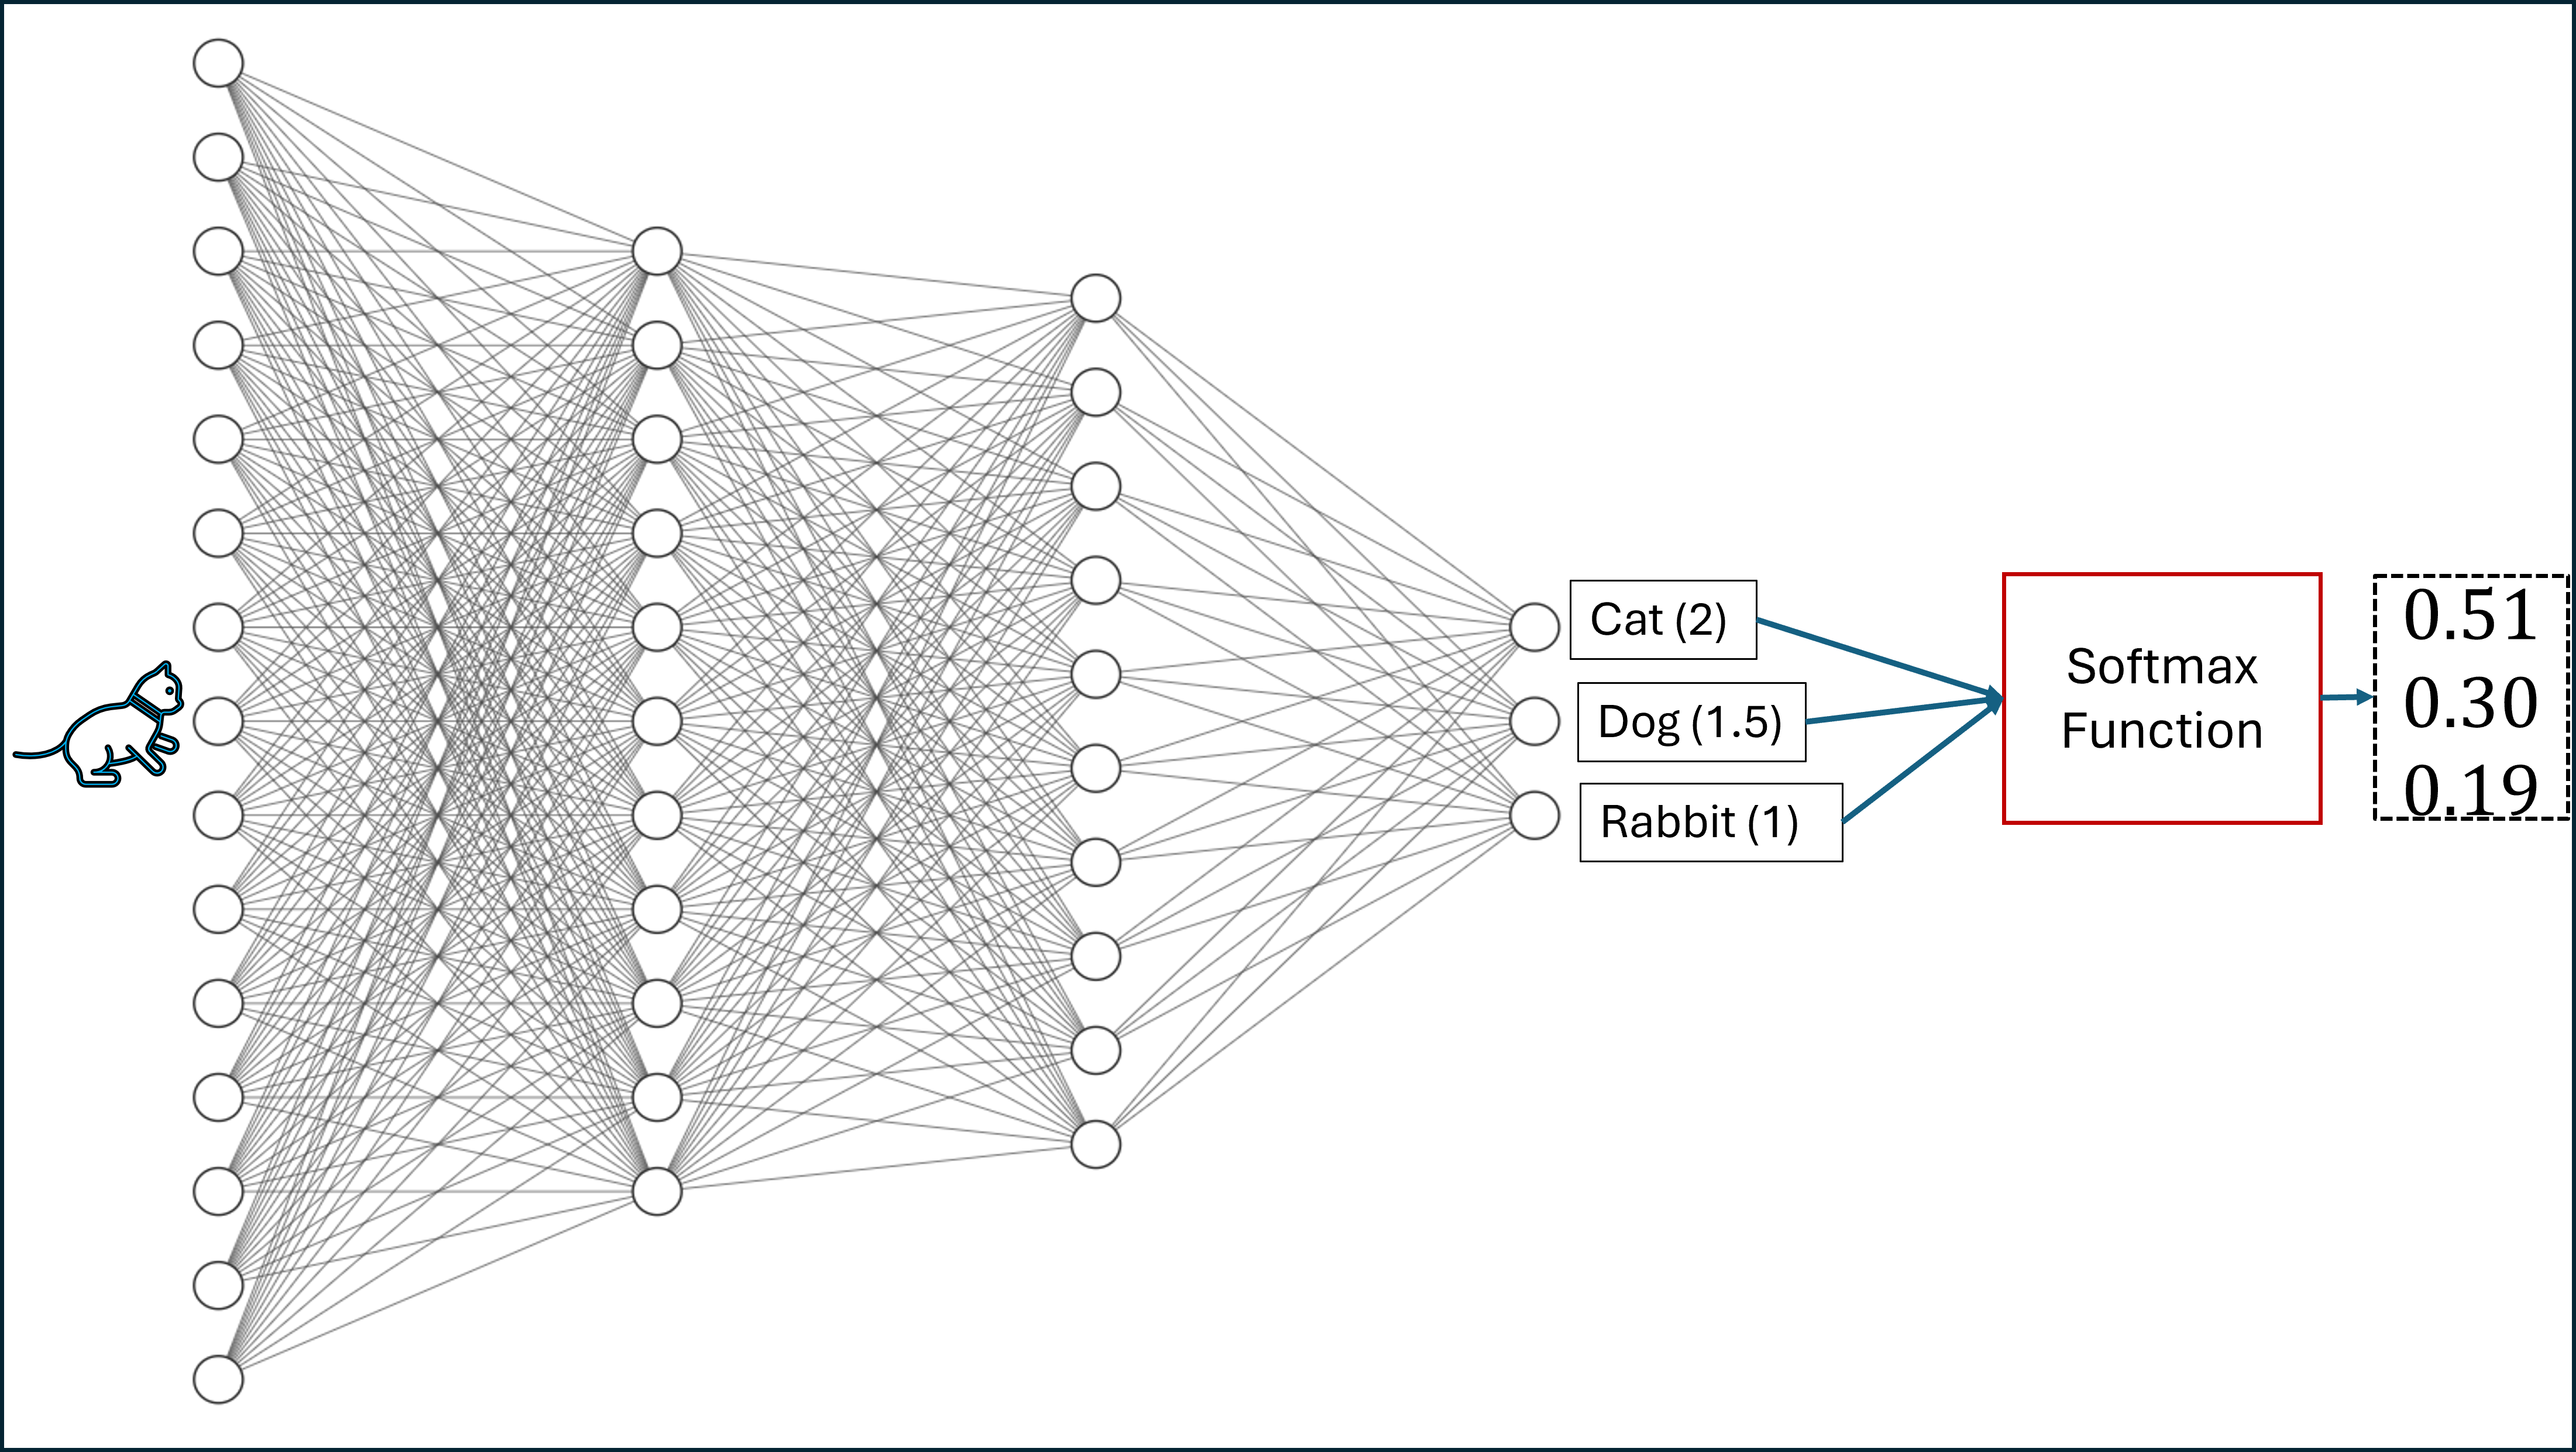
\includegraphics[width=0.65\textwidth]{imgs/softmax.png}
\caption{Illustration of Softmax Function for Multi-class Classification example. The neural network image was generated using NN-SVG \cite{web:NNSVG}.}\label{fig:softmax}
\end{figure}

Figure \ref{fig:softmax} shows an example of a neural network designed to classify images of animals into three categories: cats, dogs, and rabbits. When an image is fed into the neural network, the output layer provides raw scores (logits) for each class. Suppose the logits for a given image are 2 for cats, 1.5 for dogs, and 1 for rabbits. After applying the Softmax function (see Equation \ref{eqn:softmax}), the probabilities for each class are 0.51 (51\%), 0.30 (30\%), and 0.19 (19\%) respectively.

These probabilities sum to 1, making it possible to interpret them as the likelihood of the image belonging to each class. In this example, the neural network predicts that the image is most likely a cat with a 51\% probability.

\vspace{0.5em} 
\noindent Softmax function ကို Multi-Class Classification ပုစ္ဆာများအတွက် တည်ဆောက်သော Neural Network ၏ output layer တွင် အသုံးပြုသည်။ ၄င်း function သည် output layer မှ ရရှိသော အကြမ်း ရလဒ်များကို probability တန်ဖိုးများ အဖြစ် ပြောင်းပေးသည်။ 

ဥပမာ -- ဓါတ်ပုံတစ်ပုံကို ကြောင်၊ ခွေး နှင့် ယုန် အဖြစ် အမျိုးအစား ခွဲခြားပေးမည့် Neural Network တစ်ခုကို တည်ဆောက်ကြသည် ဆိုပါစို့။ Neural Network ၏ output layer မှ  တိရစ္ဆာန် အမျိုးအစား တစ်ခုချင်းစီအတွက် ရလဒ် အမှတ်များ ထုတ်ပေးသည်။ ထို့နောက် ပုံ \ref{eqn:softmax} တွင် ပြသထားသည့်အတိုင်း Softmax function မှ အဆိုပါ ရမှတ်များကို  probability တန်ဖိုးများ အဖြစ် ပြောင်းပေးသည်။ ရာခိုင်နှုန်းများ၏ ပေါင်းခြင်းမှာ တစ် ဖြစ်ပြီး ယခု ပုစ္ဆာတွင် ပေးထားသည့် ဓါတ်ပုံ သည် ကြောင်ဖြစ်နိုင်ချေ ၅၁ ရာခိုင်နှုန်း ၊ ခွေးဖြစ်နိုင်ချေ ၃၀ ရာခိုင်နှုန်းနှင့် ယုန်ဖြစ်နိုင်ချေ ၁၉ ရာခိုင်နှုန်း ရှိသည်။ 


\subsection{ReLU (Rectified Linear Unit) Function}
The ReLU function, as illustrated in Figure \ref{fig:relu}, returns the input if it's positive, otherwise, it returns zero. It's widely used in hidden layers of neural networks and has been found to accelerate convergence during training. Mathematically, 

\begin{equation}\label{eqn:relu}
    h_{ReLu}(z) = \max(0, z)
\end{equation} where $z$ is the pre-activation value. 

\begin{figure}[h]%
\centering
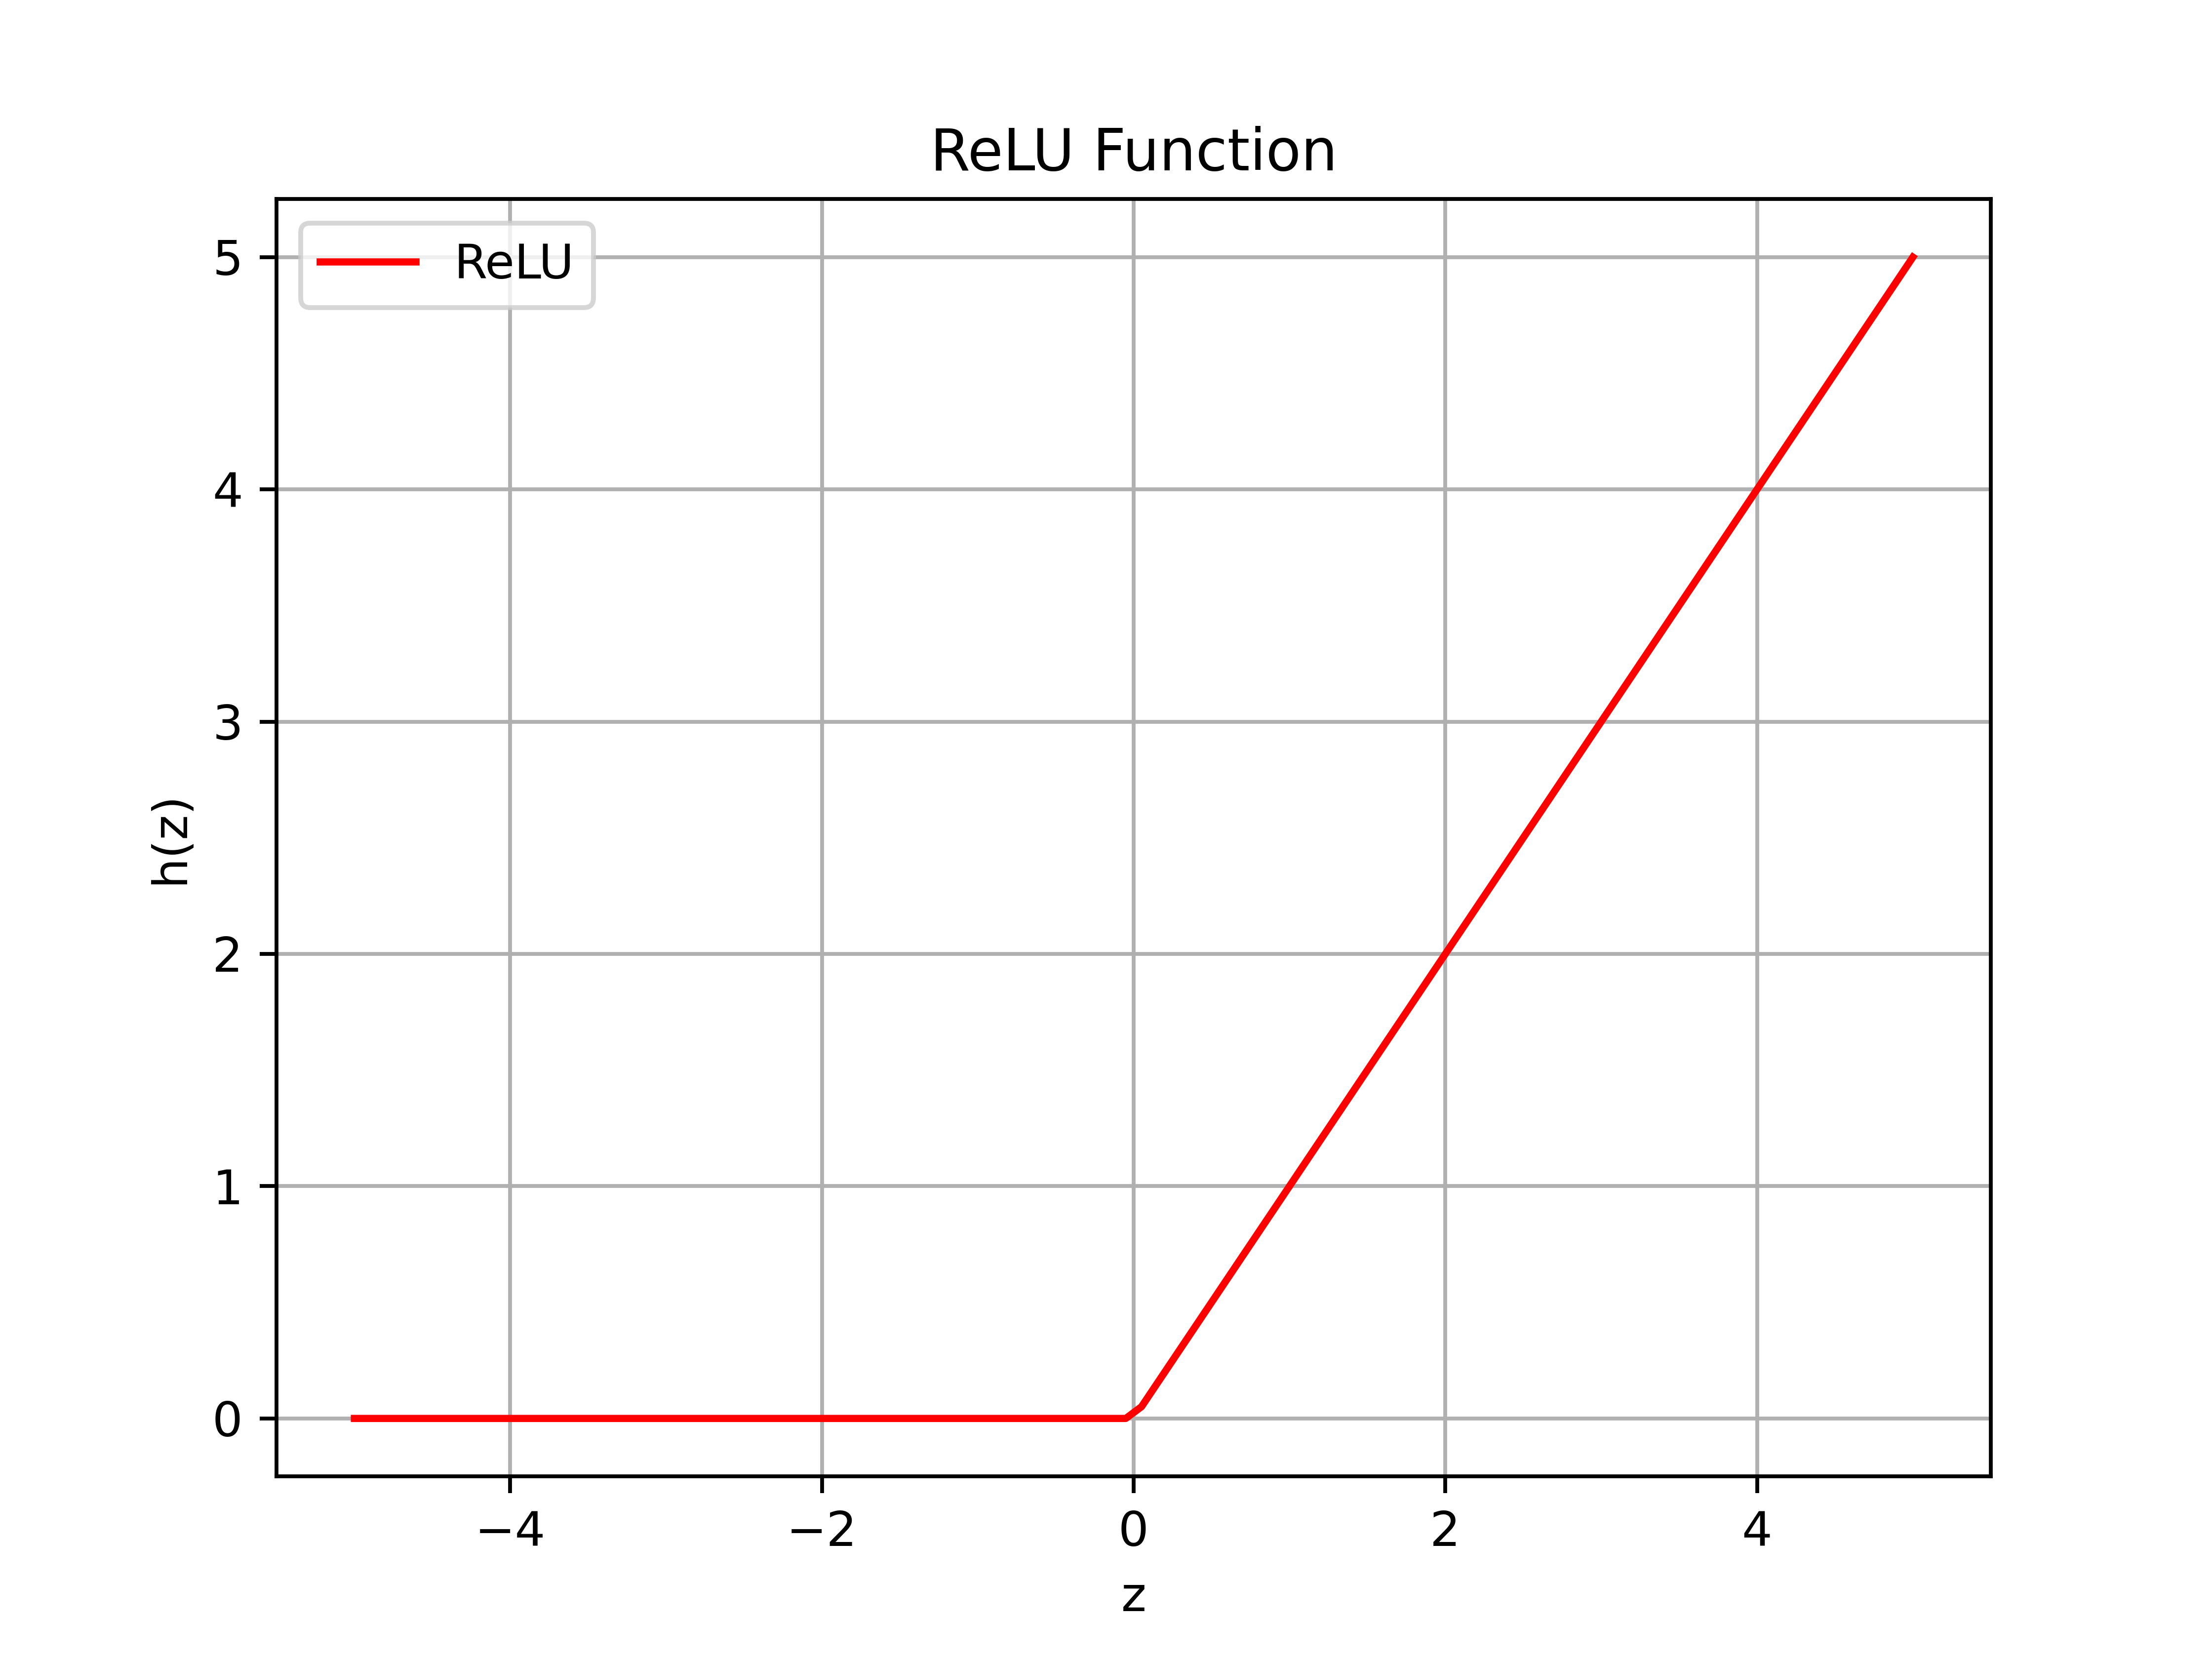
\includegraphics[width=0.65\textwidth]{imgs/relu_fun.png}
\caption{Illustration of ReLU Function. Image is generated using Python}\label{fig:relu}
\end{figure}

ReLU function ကို neural network ၏ hidden layer များအတွက် အဓိက အသုံးပြုသည်။ ဤ function (ညီမျှခြင်း- \ref{eqn:relu})သည် သုညထက်ကြီးသည့် input များအတွက် မူလတန်ဖိုးကို ပြန်ထုတ်ပေးသည်။ 

\subsection{Hyperbolic Tangent (tanh) Function} 

The hyperbolic tangent function, commonly denoted as $h_{tanh}(z)$ , is a mathematical function that maps input values to the range, $[-1,1]$ as shown in Figure \ref{fig:tanh}. It is similar to the sigmoid function but has a wider range and outputs negative values for negative inputs.  

\begin{equation}\label{eqn:tanh}
    h_{tanh}(z) = \frac{exp(z) - exp{-z}}{exp(z) + exp(-z)}
\end{equation} where $z$ is the pre-activation value. 

The tanh function is often used in hidden layers of neural networks as an activation function. It has been found to perform well in practice and is particularly useful when the data has zero mean, as it maps negative inputs to negative outputs and positive inputs to positive outputs, preserving the sign of the input.

\begin{figure}[h]%
\centering
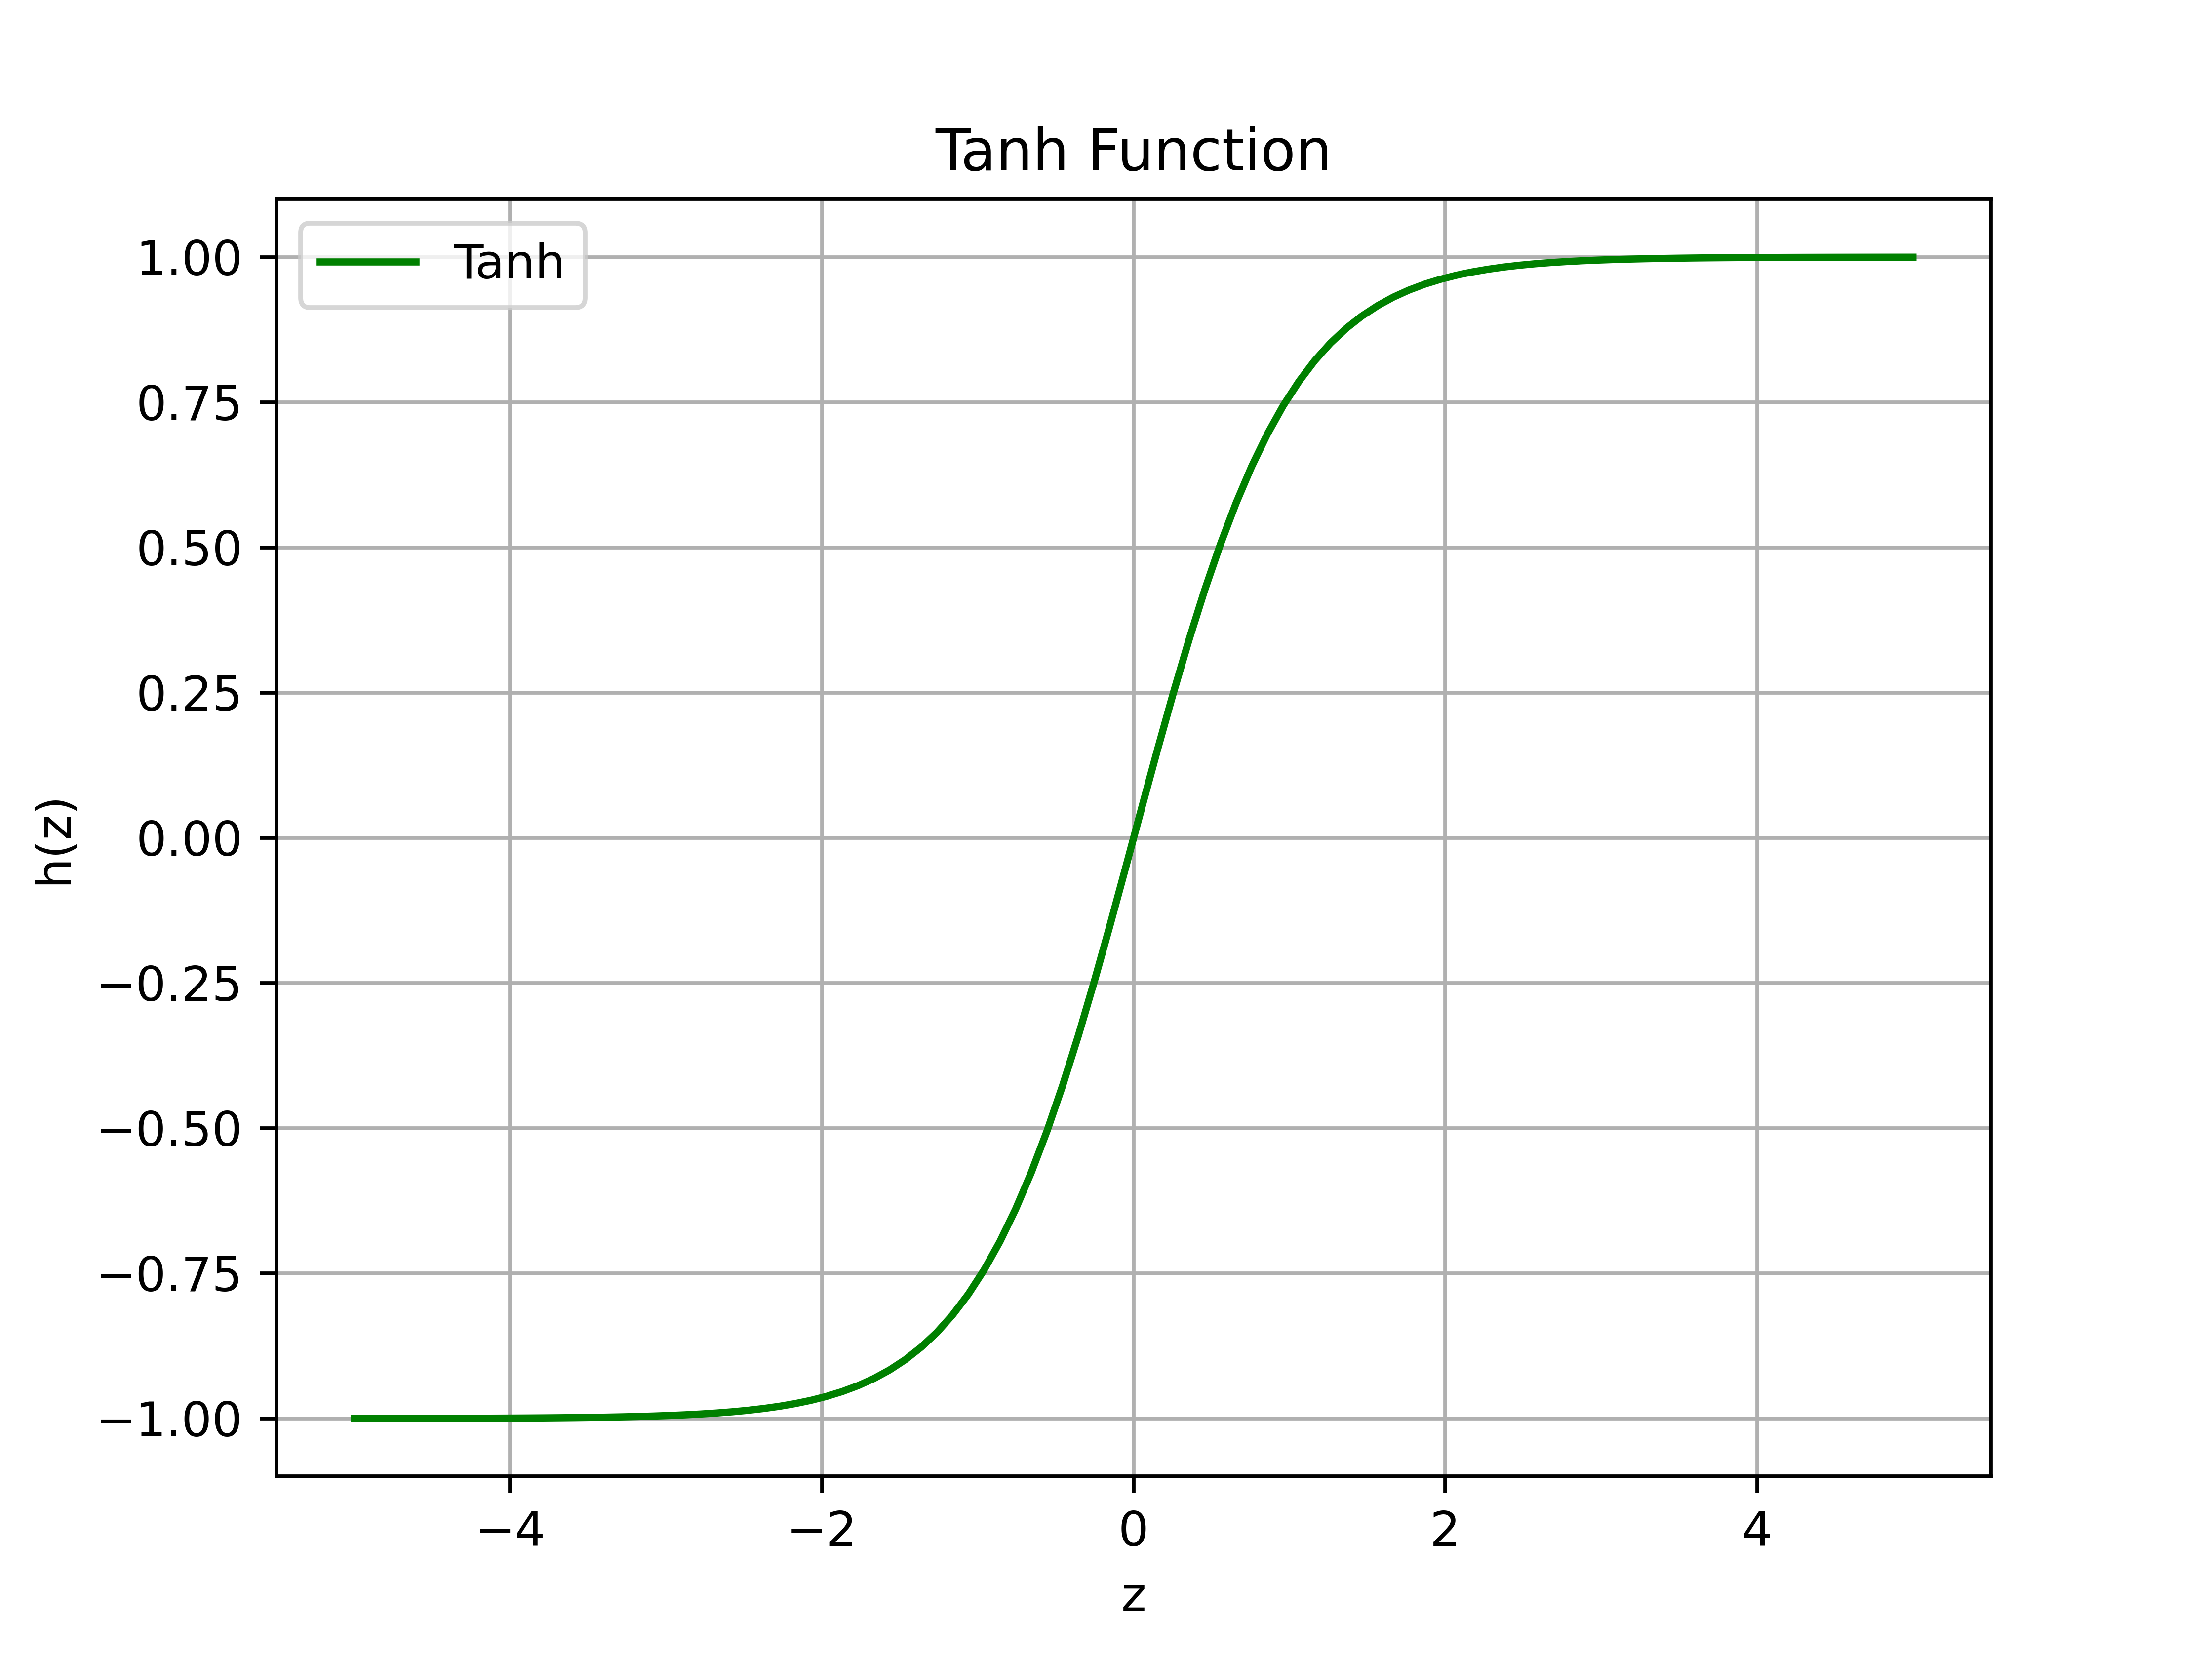
\includegraphics[width=0.65\textwidth]{imgs/tanh_fun.png}
\caption{Illustration of Hyperbolic Tangent (tanh) Function. Image is generated using Python.}\label{fig:tanh}
\end{figure}

Hyperbolic Tangent (tanh) Function သည် sigmoid Function နှင့် ဆင်တူသည်။ သို့သော် ပုံ (\ref{fig:tanh}) တွင်ပြသထားသည့် အတိုင်း $h_{tanh}(z)$ ၏ တန်ဖိုး သည် အနှုတ် တစ်နှင့် အပေါင်းတစ် အကြားတွင် ရှိသည်။ ထို့အပြင် အနှုတ်တန်ဖိုးရှိသည့် $z$ တန်ဖိုးများအတွက် အနှုတ် တန်ဖိုးကို ထုတ်ပေးပြီး သုညထက်ကြီးသည့် $z$ တန်ဖိုးများအတွက် အပေါင်းတန်ဖိုးကို ထုတ်ပေးရာ မူလ လက္ခဏာ တန်ဖိုးကို ထိန်းသိမ်းထားသည်ဟု ဆိုရမည်။ 
tanh function သည် လက်တွေ့ ပုစ္ဆာများတွက်ချက်ရာတွင် ရလဒ်ကောင်းများ ရရှိသည်ကို တွေ့ရပြီး hidden layer များအတွက် အဓိက အသုံးပြုသည်။

\newpage
\section{Forward Propagation}\label{sec:FProp}
Forward propagation is the process by which input data passes through the network layers, moving from left to right, to produce an output. It involves a series of mathematical operations that transform the input data, step by step, through each layer of the network. At the start of training, the neural network's weights and biases are typically unknown and initialized randomly.

\vspace{1.5em} 

\begin{figure}[h]%
\centering
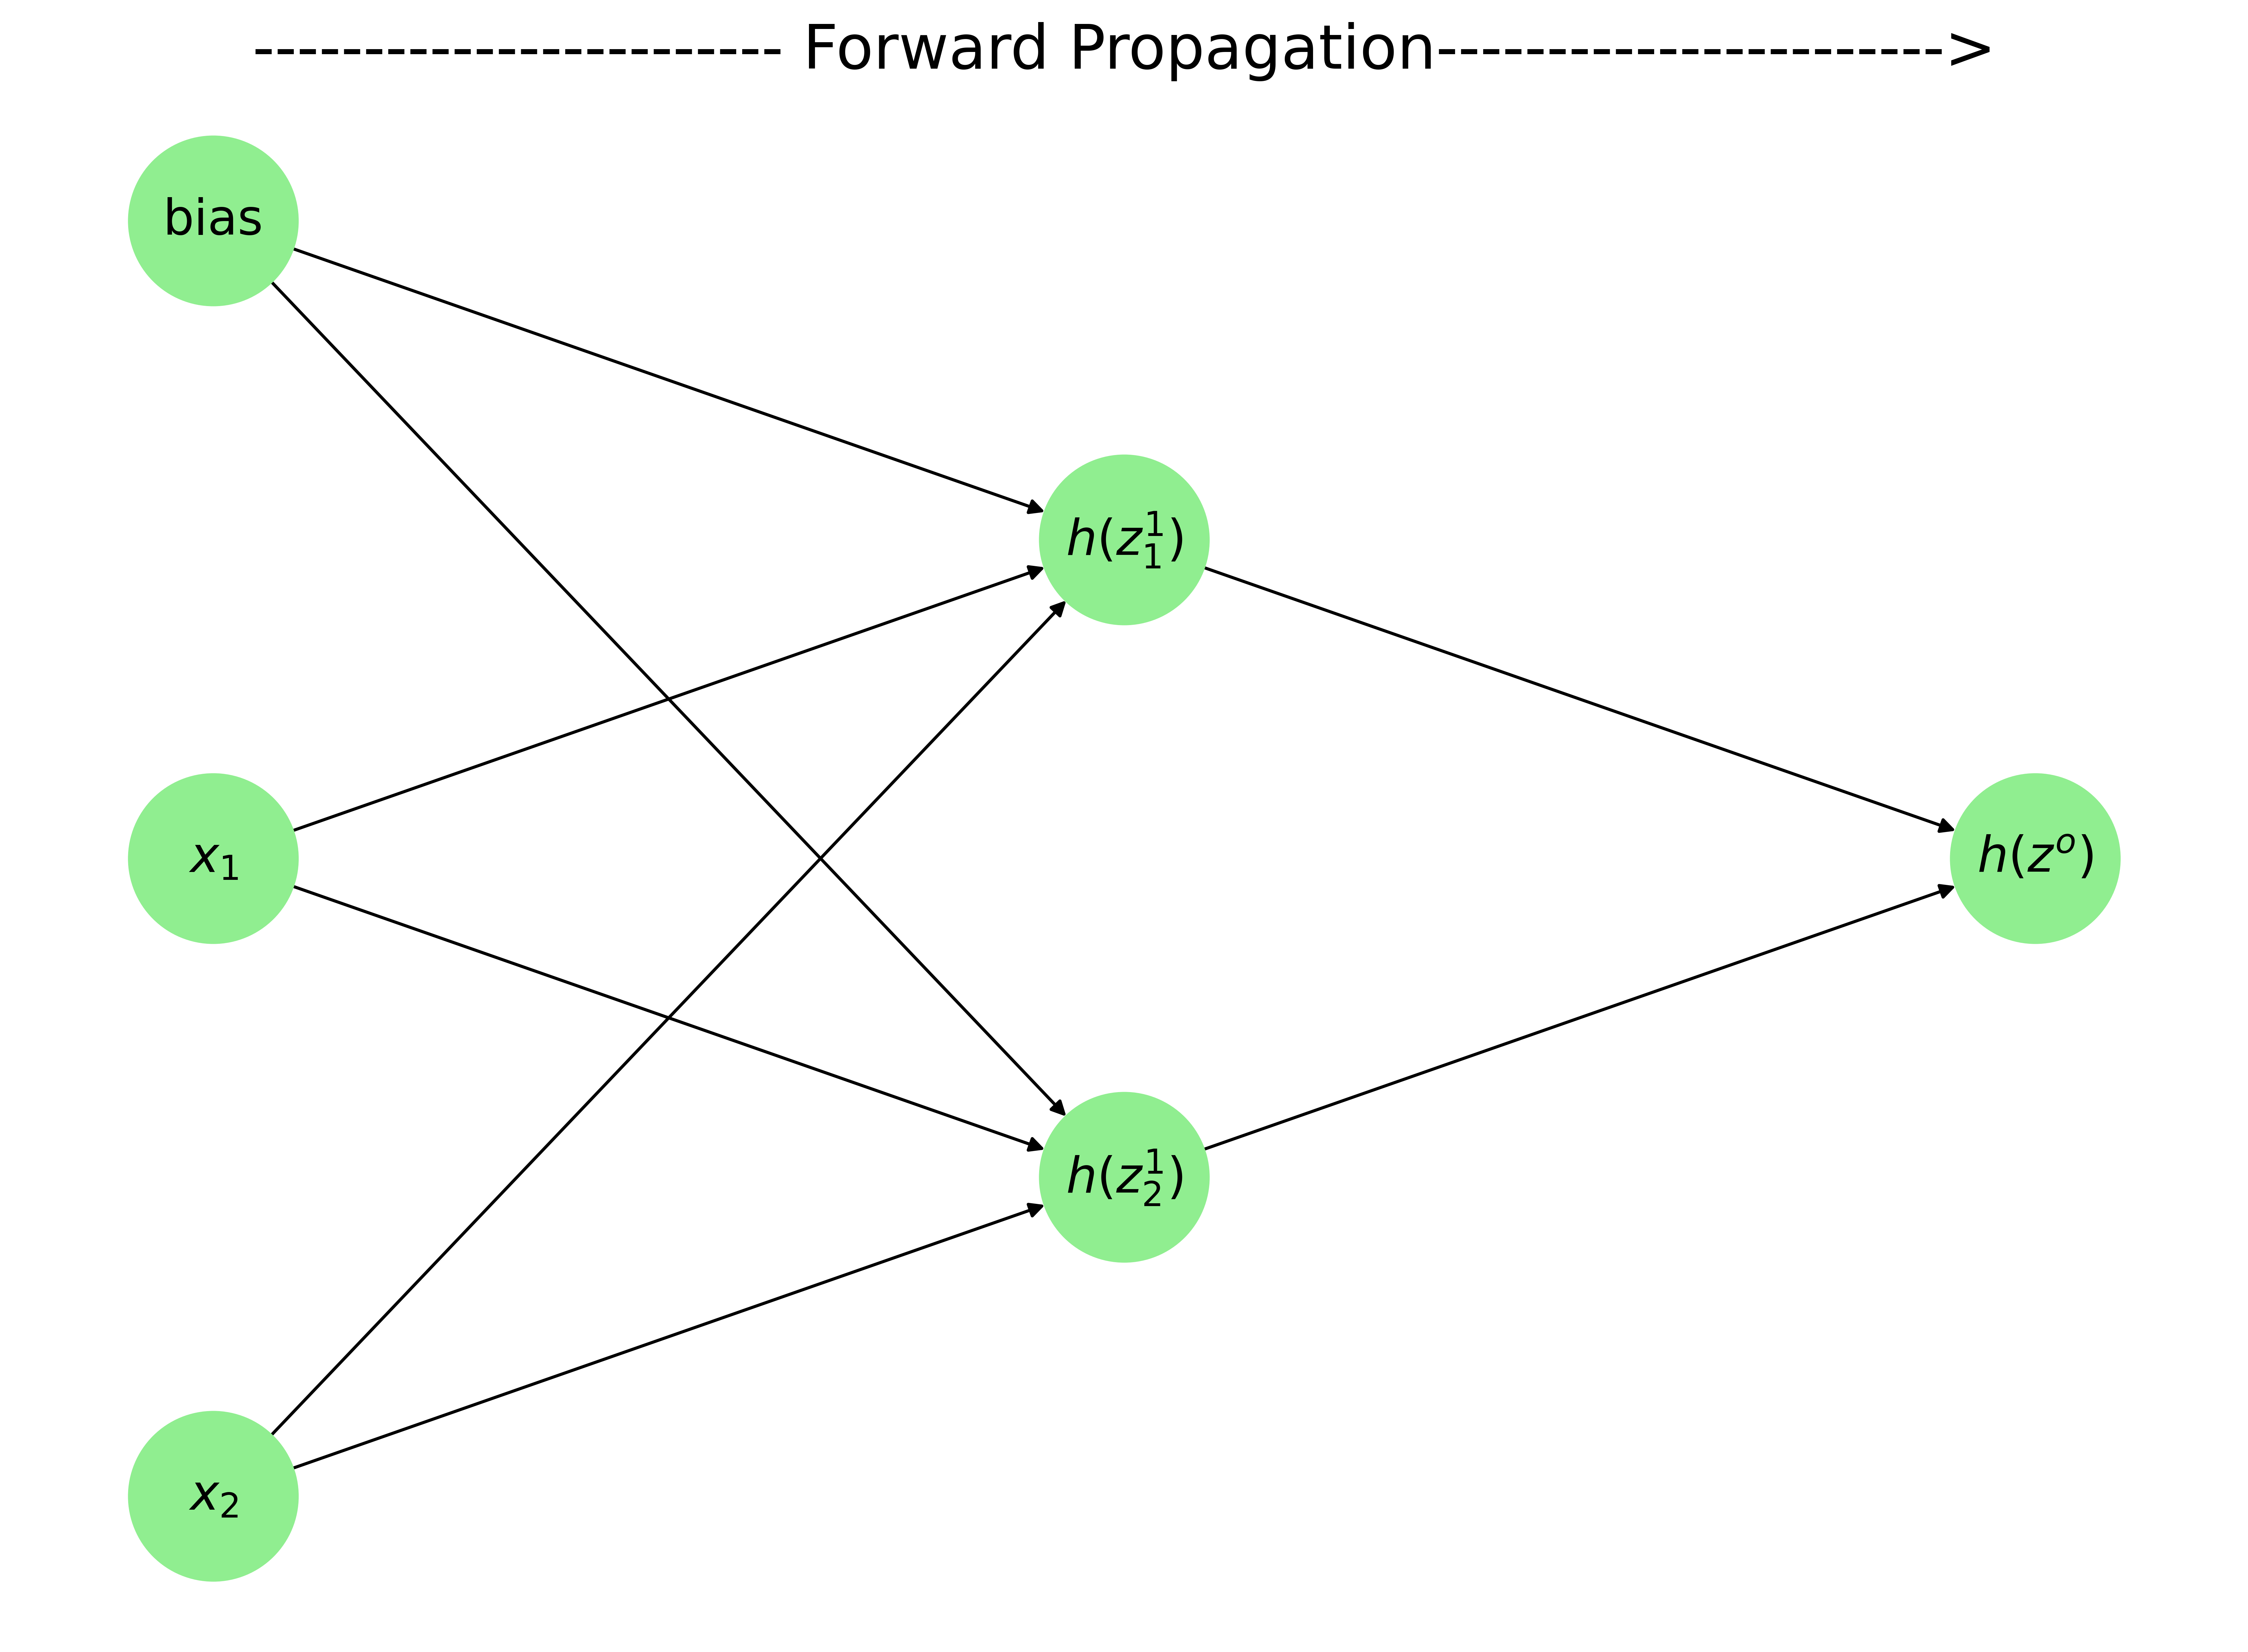
\includegraphics[width=0.75\textwidth]{imgs/fw_eg.png}
\caption{Multi-Layer Perception with one hidden layer and two input features. Image is generated using Python networkX Library}\label{fig:mlp_fwprop}
\end{figure}

\noindent Let's consider a simple example with a single hidden layer as shown in Figure \ref{fig:mlp_fwprop}:
\begin{itemize}
  \item \textbf{Input Layer}: Suppose we have two input features, $x_1$ and $x_2$.
  \item \textbf{Hidden Layer}: The hidden layer has two neurons. Each neuron receives $x_1$ and $x_2$ as inputs and computes the pre-activation values for each neuron, $z^1_1$ and $z^1_2$. 
  \begin{eqnarray}\label{enq:z12} 
    z^1_1  &=& \omega_{11} x_1 + \omega_{12}x_2 + b_1 \\
    z^1_2 &=& \omega_{21} x_1 + \omega_{22}x_2 + b_2
  \end{eqnarray} where $\omega_{i1}$ are the weights associated with the input features and the neurons in the hidden layer, and $b_i$ are the bias values.
  The outputs, $z^1_1$ and $z^1_2$ are then passed through an activation function and produces: 
  \begin{eqnarray}\label{enq:a12} 
    a_1 &=& h(z^1_1)\\
    a_2 &=& h(z^1_2)
  \end{eqnarray}  

  \item \textbf{Output Layer}: The output layer has one neuron, which takes $a_1$ and $a_2$ and computes the output:
    \begin{equation} \label{enq:Poutput} 
     y  = h (z^o) \text{ where } z^o = \omega_{o1} a_1 + \omega_{o2} a_2 + b_o
    \end{equation} $z^o$  is the pre-activation value at the output layer, $\omega_{oj}$ are the weights associated with the output and the neurons in the hidden layer, and $b_o$ is the bias value.
\end{itemize}

In forward propagation, the computed $y$ represents the predicted value using random weights. 

The objective of the machine learning model is to find the parameters (weights and bias) that produce the lowest errors between the actual and predicted values. This parameters are iteratively refined through backward propagation, where the model adjusts its parameters based on the calculated errors to improve its predictive accuracy. 

\noindent ပုံ \ref{fig:mlp} သည် hidden layer တစ်ခုပါ၀င်သော Multi-layer neural network ၏ ဥပမာဖြစ်သည်။  Input layer တွင် feature နှစ်ခု $x_1$ နှင့် $x_2$ တို့ရှိပြီး အဆိုပါ feature များသည် ကြားခံ layer ၏ Input များဖြစ်သည်။  ထို့နောက် $z^1_1$ နှင့် $z^1_2$ တန်ဖိုးကို ညီမျှခြင်း (\ref{enq:z12})ကို အသုံးပြု၍ တွက်ချက်သည်။ တနည်းဆိုသော် $z^1_1$ နှင့် $z^1_2$ ၏ တန်ဖိုးများသည် မြှောက်ဖော်ကိန်းများနှင့် မြှောက်ထားသည့် input feature များ၏ စုစုပေါင်းတန်ဖိုး ဖြစ်သည်။ 

ထို့နောက်  ကြားခံ layer ၏ output များဖြစ်သည့် $a_1$ နှင့် $a_2$ ၏ တန်ဖိုးကို activation function တစ်ခုကို သုံး၍ တွက်ချက်ရမည်။ အသုံးများသည့်  function များမှာ ReLU, Sigmoid, (သို့မဟုတ်) Tanh တို့ဖြစ်ကြသည်။ အဆိုပါ $a_1$ နှင့် $a_2$ သည် Output Layer အတွက် input များ ဖြစ်သည်။ ထို့နောက် final ရလဒ် ဖြစ်သော  $y$ ၏ တန်ဖိုးကို ညီမျှခြင်း \ref{enq:Poutput} ကို အသုံးပြု၍ တွက်ချက်သည်။ Classification ပုစ္ဆာများအတွက် Output Layer တွင် softmax  activation function ကို အသုံးပြုလေ့ ရှိပြီး regression ပုစ္ဆာများအတွက် linear function , $h(z^o) = z^o$ ကို အသုံးပြုကြသည်။ 

အထက်ပါ ညီမျှခြင်းများ (\ref{enq:z12}၊ \ref{enq:Poutput}) တွင် မြှောက်ဖော်ကိန်းများ ဖြစ်သော $\omega_{i}$ နှင့် $b_i$ ၏တန်ဖိုးများကို randomly သတ်မှတ်၍ တွက်ချက်ခြင်း ဖြစ်သည်။ Forward propagation မှ ရရှိသည့် $y$ ၏ တန်ဖိုးမှာ Multi-layer neural network Model မှ တွက်ချက်ပေးသည့် ခန့်မှန်းတန်ဖိုးသာ ဖြစ်သည်။ Machine learning model များ၏ ရည်ရွယ်ချက်မှာ ခန့်မှန်းတန်ဖိုး နှင့် training ဒေတာများ၏ မူလတန်ဖိုးကြား ခြားနားချက်ကို အနည်းဆုံးဖြစ်စေသည့် မြှောက်ဖော်ကိန်း များ $\omega_{i}$ နှင့် $b_i$ တန်ဖိုးများကို ရှာရန် ဖြစ်သည်။ 

\newpage
\section{Backward Propagation}\label{sec:bProp}

Backward propagation, also known as backpropagation, involves the iterative adjustment of the model's parameters (weights and biases) based on the calculated errors between the predicted and actual outputs. The Gradient descent is one of the fundamental algorithms used for updating the parameters. 
\begin{itemize}[f1]
  \item\textbf{Loss Computation}: After forward propagation, the model's prediction, $\hat{y}$ is compared to the actual target value $y$ using a loss function (e.g., mean squared error for regression, binary cross-entropy for binary classification, categorical cross-entropy for multi-class classification). This loss function computes the disparity between the predicted and actual outputs. 
  \item \textbf{Backpropagate Errors}: Once the loss is computed, the algorithm works backward through the network to calculate the gradient of the loss function with respect to each parameter. 
      \begin{itemize}
        \item \textbf{Output Layer}: Compute the gradients of weights and bias in the output layer using the chain rule
        \begin{eqnarray}\label{eqn:gradient1}
        % \nonumber to remove numbering (before each equation)
          \frac{\delta Loss}{\delta \omega_o} &=& \frac{\delta Loss}{\delta z^o } . \frac{\delta z^o}{\delta \omega_o}\\
         \frac{\delta Loss}{\delta b_o} &=& \frac{\delta Loss}{\delta z^o } . \frac{\delta z^o}{\delta b_o}
        \end{eqnarray}
        \item \textbf{Hidden Layer}: Compute the gradients of weights and bias in the hidden layer 
        \begin{eqnarray}\label{eqn:gradient2}
        % \nonumber to remove numbering (before each equation)
          \frac{\delta Loss}{\delta \omega_{hidden}} &=& \frac{\delta Loss}{\delta z^{hidden} } . \frac{\delta z^{hidden}}{\delta \omega_{hidden}}\\
         \frac{\delta Loss}{\delta b_{hidden}}           &=& \frac{\delta Loss}{\delta z^{hidden} } . \frac{\delta z^{hidden}}{\delta b_{hidden}}
        \end{eqnarray}
      \end{itemize}
  \item \textbf{Update Weights and Biases}: Adjust the weights and biases in both the output and hidden layers using the computed gradients and a learning rate. This step involves moving in the opposite direction of the gradients to minimize the loss function. 
      \begin{eqnarray}\label{eqn:update}
        % \nonumber to remove numbering (before each equation)
          \omega_o^{new} &=& \omega_o^{old} - \text{learning rate} \times \frac{\delta Loss}{\delta \omega_o}\\
          b_o^{new}          &=& b_o^{old} - \text{learning rate} \times \frac{\delta Loss}{\delta b_o}\\
          \omega_{hidden}^{new} &=& \omega_{hidden}^{old} - \text{learning rate} \times \frac{\delta Loss}{\delta \omega_{hidden}}\\
          b_{hidden}^{new}          &=& b_{hidden}^{old} - \text{learning rate} \times \frac{\delta Loss}{\delta b_{hidden}}   
        \end{eqnarray}
\end{itemize}

Both forward and backward propagation are repeated for multiple \textbf{epochs} until the model converges or until a stopping criterion is met.

\begin{definition}\label{def:epoch}
An \textbf{epoch} refers to one complete pass through the entire training dataset. During each epoch, the neural network performs forward and backward propagation (calculating predictions, computing loss, and updating weights) for every sample in the training dataset.
\end{definition}

\newpage
\noindent Neural Network Model တစ်ခုကို Training ပြုလုပ်ရာတွင် forward နှင့် backward propagation ကို ကြိမ်ဖန်များစွာ ပြုလုပ်ပြီး ခန့်မှန်းတန်ဖိုးနှင့် မူလတန်ဖိုး၏ ခြားနားချက် အနည်းဆုံးဖြစ်စေမည့် $\omega_{i}$ နှင့် $b_i$ ၏ တန်ဖိုးများကို ရှာဖွေရသည်။ Forward propagation အဆင့်တွင် $\hat{y}$ ၏ တန်ဖိုးကို တွက်ချက်နိုင်ရန်အတွက်  neural network ၏ input layer မှ output layer တဆင့်ချင်း (ဘယ်မှညာသို့) တွက်ချက်ရသည်။ 

Backward propagation အဆင့်တွင်မူ output layer မှ  input layer သို့ (ညာမှ ဘယ်သို့) ပြန်သွားပြီး layer တစ်ခုချင်းစီတွင် ရှိသည့် Parameter များ၏ gradients တန်ဖိုးများကို ညီမျှခြင်း \ref{eqn:gradient1} နှင့် \ref{eqn:gradient2} တို့ကို အသုံးပြု၍ တွက်ချက်သည်။ ထို့နောက် $\omega_{i}$ နှင့် $b_i$ များ၏ တန်ဖိုးကို ညီမျှခြင်း \ref{eqn:update} ကို အသုံးပြု၍ update ပြုလုပ်ပေးရသည်။ 

Forward နှင့် backward propagation process - ၂ ခု လုံးပါ၀င်သော Cycle တစ်ခုကို epoch ဟုခေါ်ဆိုပြီး Neural Network Model များ တည်ဆောက်ရာတွင် Programmer/developer မှ epoch အရေအတွက်ကို သတ်မှတ်ပေးရန် လိုအပ်သည်။ 

\newpage
\section{Practical Implementation}\label{sec:hands-on}
In this section, two practical projects are presented to reinforce the concepts learned in the previous sections. These projects are designed to provide hands-on experience and deepen your understanding through real-world applications. By working through these projects, you will be able to apply the theoretical knowledge in practical scenarios, thereby solidifying your learning and enhancing your skills. 

Walk-through videos are provided via the author's YouTube channel \cite{web:myoYouTube}. You can watch the videos while reading and implementing the codes along.

ဤအခန်းတွင် လက်တွေ့  industry တွင် အသုံး၀င်သည့် project နှစ်ခုကို Neural Network အသုံးပြု၍ တည်ဆောက်ပုံ တည်ဆောက်နည်း အဆင့်ဆင့်ကို ဖော်ပြသွားမည် ဖြစ်သည်။ Deep Learning ကို လေ့လာရာတွင် project များကို လက်တွေ့  လိုက်ပါ လေ့ကျင့်ရန် လိုအပ်ပါသည်။ ဤ လေ့ကျင့်ခန်းများကို လေ့လာရာတွင် အထောက် အကူဖြစ်စေရန်အတွက် project ကို ရှင်းပြသည့် video များကို YouTube Channel တွင် တင်ပေးထားပြီး ဖြစ်သည်။ သက်ဆိုင်ရာ Project အလိုက် ပေးထားသည့် လင့်တွင် သွားရောက် ကြည့်ရှု့နိုင်သည်။ 

\subsection{Regression: Resale House Price Prediction}\label{sec:SGHDB}

House price prediction is a significant application of machine learning with substantial implications for various stakeholders in the real estate market. The deployment of these models into commercial platforms enhances decision-making processes, market analysis, and strategic planning. Leveraging large datasets and advanced algorithms, machine learning (ML) models have significantly transformed the landscape of house price prediction, yielding remarkably accurate predictions.

In today's digital landscape, numerous real estate websites and applications integrate ML models to provide price estimates for listed properties. This integration not only elevates user experience and engagement but also empowers buyers and sellers to make informed decisions. Additionally, it enables real estate agents to offer enhanced services and assists investors in identifying opportunities within the market. Continuously improving ML models for higher accuracy is a collaborative effort between academia and industry. Real estate data is dynamic, with various factors influencing prices differently across regions. Therefore, it is essential to develop models tailored to each market's unique characteristics.

In Singapore, an HDB (Housing and Development Board) estate typically refers to a large residential area comprising multiple HDB blocks. Each block is a high-rise building containing numerous housing units, commonly known as HDB flats or apartments.  All HDB properties in Singapore typically have a 99-year lease term.

First-time buyers acquire their properties directly from the Singapore government, while resale transactions involve the buying and selling of units among Singapore residents. Each transaction is recorded by the Singapore Housing and Development Board to track ownership. In earlier records, the approval date by HDB is considered the transaction date, but after 2014, the registration date is recorded. These two dates are typically within a month of each other, resulting in minimal fluctuation. However, the resale prices recorded by HDB should be considered indicative only, as the actual resale prices agreed upon between buyers and sellers depend on many factors. Being able to estimate the resale price based on the properties of a flat, such as location, area, and other factors, helps both buyers and sellers make informed decisions.

This section explains, step by step, how to develop a Neural Network (deep learning) model for predicting resale prices of public housing flats (HDB flats) in Singapore. 

\begin{remark}
This work is inspired by a project assignment given to my students during the Supervised Machine Class (iSTAR) of 2024. In this course, students were tasked with developing a regression model to predict housing prices for houses or flats in the region. While the codes and explanations are my original work, the project context was developed as part of the coursework to provide practical learning experiences.
\end{remark}

Real estate Online Platform များတွင်  Machine learning model များကို ထည့်သွင်း အသုံးပြုလာနိုင်ခြင်းသည် အိမ်ခြံမြေစျေးကွက်ကို စိတ်၀င်စားသူများအတွက် အရေးပါသော အရွေ့ တစ်ခု ဖြစ်သည်။ ဒေတာ အချက်အလက်များ တနေ့တခြား များပြားလာခြင်း နှင့် အတူ အချက်အလက်မှန်ကန်သည့် ဒေတာများကို အစိုးရ website များ အပါအ၀င် အဖွဲ့အစည်းအမျိုးမျိုးက အများပြည်သူ အသုံးပြုနိုင်အောင်ဖွင့်ပေးလာကြသည်။ ထိုသို့ ဒေတာများ အလွယ်တကူ ရရှိနိုင်ခြင်း၊ ကွန်ပြူတာများ အဆင့်မြင့်လာခြင်းတို့သည် အိမ်ခြံမြေ နှင့် တိုက်ခန်းများ၏ စျေးနှုန်းခန့်မှန်းရန်အတွက် ပိုမိုကောင်းမွန်သည့် Machine learning model များ တည်ဆောက်ရန် အထောက်အပံ့ကောင်းများ ဖြစ်သည်။ 

အိမ်ခြံမြေစျေးကွက်၏ သဘော သဘာ၀မှာ နေရာဒေသတစ်ခုနှင့် တစ်ခု အပေါ်မူတည်၍ အချက်အလက်များ ကွဲပြားကြသည်။ သို့ဖြစ်ရာ Machine learning model တစ်ခုထဲကို နေရာအမျိုးမျိုးတွင် အသုံးပြုရန်မှာ မဖြစ်နိုင်ပေ။ နိုင်ငံ (သို့ မဟုတ်) မြို့နယ် အလိုက် ရရှိနိုင်သော ဒေတာအချက်အလက်များကို အသုံးပြု၍ တည်ဆောက်မှသာလျှင် ပို၍ တိကျသော စျေးနှုန်းခန့်မှန်းချက်များကို ရရှိနိုင်မည် ဖြစ်သည်။ 

Singapore နိုင်ငံတွင် အများပြည်သူများ သက်သက်သာသာနှင့် ၀ယ်ယူနေထိုင်နိုင်ရန် အစိုးရအဖွဲ့အစည်းတစ်ခုဖြစ်သည့် HDB (Housing and Development Board) မှ တာ၀န်ယူ ဆောက်လုပ်သည့် တိုက်ခန်းများကို HDB တိုက်ခန်းများဟု ခေါ်ဆိုကြသည်။ မြို့နယ်အလိုက်  HDB အိမ်ယာများစွာ ရှိပြီး အိမ်ယာတစ်ခုတွင် အထပ်မြင့် အဆောက်အအုံတစ်ခုမက ပါ၀င်သည်။ အဆိုပါ အဆောက်အအုံများကို Singapore အစိုးရမှ ပိုင်ဆိုင်ပြီး ပြည်သူကို ရောင်းချသည့် သက်တမ်းမှာ ၉၉ နှစ်သာ ဖြစ်သည်။ တိုက်သက်တမ်းလွန်သည့် တိုက်ခန်းများကို အစိုးရက ဖြိုဖျက်ပြီး အသစ်ပြန်လည်ဆောက်လုပ်လေ့ရှိသည်။ အသစ်ဆောက်လုပ်ပြီးစီးသည့် HDB တိုက်ခန်းများကို Singapore အစိုးရထံမှသာ တိုက်ရိုက် ၀ယ်ဆိုနိုင်သည်။ သတ်မှတ် ကာလတစ်ခု  (များသောအားဖြင့် ၅ နှစ်) ကျော်လွန်သွားပါက HDB တိုက်ခန်းဟောင်းများကို နေထိုင်သူ အချင်းချင်းကြား ပြန်လည်ရောင်းချခြင်း၊ ၀ယ်ယူခြင်းများ ပြုလုပ်နိုင်သည်။ 

သို့သော် အရောင်းအ၀ယ် ပြုလုပ်မည်ဆိုပါက Singapore အစိုးရ (HDB) ထံမှ တရား၀င် ခွင့်ပြုချက်ရယူရန်လိုအပ်သည်။ အဆိုပါ အရောင်းအ၀ယ်မှတ်တမ်းတိုင်းကို HDB တွင် စနစ်တကျ စာရင်းသွင်းထားရှိသည်။ အစောပိုင်း စာရင်းသွင်းချက်များတွင် HDB မှ ခွင့်ပြုပေးလိုက်သည့် နေ့ကို အရောင်းအ၀ယ်ပြုလုပ်သည့်နေ့ဟု သတ်မှတ်ခဲ့ကြသော်လည်း နောက်ပိုင်း မှတ်တမ်းများတွင်မူ HDB တွင် မှတ်တမ်းတင်သည့်နေ့ကို အရောင်းအ၀ယ်ပြုလုပ်သည့်နေ့ဟု သတ်မှတ်သည်။ ယေဘူယျအားဖြင့်  HDB မှ ခွင့်ပြုပေးလိုက်သည့် နေ့နှင့် မှတ်တမ်းတင်သည့်နေ့မှာ တစ်လအတွင်းဖြစ်သဖြင့် ကြားထဲတွင် စျေးနှုန်း အပြောင်းအလဲ ဖြစ်လေ့မရှိပါ။ သို့သော် ရောင်းသူနှင့် ၀ယ်သူ အကြားသဘောတူညီချက်များကို မူတည်၍ HDB ၏ မှတ်တမ်းရှိ စျေးနှုန်းများနှင့် ပြင်ပပေါက်စျေးများသည် အနည်းငယ် ကွာဟနိုင်သည်။ 

ဤသင်ခန်းစာတွင် Singapore နိုင်ငံရှိ HDB တိုက်ခန်းများ၏ စျေးနှုန်းကို ခန့်မှန်းသည့် Neural Network Model တစ်ခုအား Keras Library ကို အသုံးပြု၍ တည်ဆောက်သည့် အဆင့်ဆင့်ကို ရှင်းပြသွားမည်။ 

\subsubsection{Dataset}

The dataset used for this project is obtained from the Singapore government's open data portal \cite{web:SGdata}, which provides various datasets relevant to different aspects of public administration, urban planning, health, transportation, and other sectors managed by the government. Using a reliable data source is crucial for building an accurate and robust machine learning model.

The dataset includes detailed information on resale transactions of HDB flats between January 1, 2017, and March 30, 2024. The dataset contains 175,672 rows and 11 columns and was downloaded on May 23, 2024.  Further details regarding the dataset are outlined in Table \ref{tab:data_attributes}. 

\vspace{0.5em}

\begin{table}[h]
\centering
\caption{Data Attributes of Singapore HDB Flat (January - 2017 to March  - 2024}
\label{tab:data_attributes}
{\scriptsize
\begin{tabular}{|c|l|l|l|l|}
\hline
\textbf{Num} & \textbf{Data Attributes} & \textbf{Column Name} & \textbf{Data Type} & \textbf{Description} \\ \hline
1 & Month & month & Text (Date-Time) & Month and Year of sale \\ \hline
2 & Town & town & Text & Designated residential area \\ \hline
3 & Flat type & flat\_type & Text & Classification of units by room size \\ \hline
4 & Block & block & Text & The Block number where the unit sold located \\ \hline
5 & Street name & street\_name & Text & Street name of the unit sold located \\ \hline
6 & Storey range & storey\_range & Text & Estimated range of floors the unit sold was located on \\ \hline
7 & Floor area sqm & floor\_area\_sqm & Numeric & Total interior space within the unit, measured in square meters \\ \hline
8 & Flat model & flat\_model & Text & Classification of units by generation \\ \hline
9 & Lease commence date & lease\_commence\_date & Numeric & Starting point of a lease agreement (Year) \\ \hline
10 & Remaining lease & remaining\_lease & Text & Remaining amount of time left on the lease (Years and Months) \\ \hline
11 & Resale price & resale\_price & Numeric & Resale Price of the flat sold \\ \hline
\end{tabular}}
\end{table}

\noindent ယခု Project တွင် အသုံးပြုသည့် ဒေတာကို Singapore အစိုးရ၏ open data portal \cite{web:SGdata} မှ ရယူထားခြင်းဖြစ်သည်။ အဆိုပါ website ကို Singapore အစိုးရ အဖွဲ့အစည်းတစ်ခုဖြစ်သည့် GovTech မှ တည်ထောင်ထားခြင်းဖြစ်ပြီး Singapore ၀န်ကြီးဌာန အချို့ နှင့် အစိုးရ အဖွဲ့အစည်းများ၏ ဒေတာများကို ပြည်သူအများ အသုံးပြုနိုင်ရန် တင်ပေးထားသည်။ AI နှင့်  Machine Learning Project များ ပြုလုပ်ရာတွင် ယုံကြည် စိတ်ချရသည့် ဒေတာ အချက်အလက်များကို ရယူနိုင်ရန် အရေးကြီးသည်။ 

ဤ dataset ကို ၂၀၂၄ ခုနှစ် မတ်လ ၂၃ ရက်နေ့တွင် အထက်ပါ website မှ download ရယူခဲ့ပြီး ၄င်း dataset တွင် ၂၀၁၇ ဇန်န၀ါရီလ ၁ ရက်မှ ၂၀၂၄ မတ်လ ၃၁ ရက်နေ့အထိ ရောင်းချထားသော Singapore HDB တိုက်ခန်းများ၏ အရောင်းစာရင်းများ ပါ၀င်သည်။ စုစုပေါင်းပါ၀င်သည့် အရောင်း တိုက်ခန်း အရေအတွက်မှာ တစ်သိန်း ခုနစ်သောင်း ငါးထောင် ခြောက်ရာ ခုနစ်ဆယ့် နှစ်ခု (၁၇၅,၆၇၂)  ဖြစ်ပြီး ရောင်းချမှုအတွက် စာရင်းသွင်းသည့် ခုနှစ်နှင့်လ၊ တိုက်ခန်း အကျယ်အ၀န်း၊ အမျိုးအစား၊ တည်နေရာ စသည်ဖြင့် Column -၁၁ ခု ပါ၀င်သည်။ အထက်ပါ ဇယားတွင် ဖော်ပြထားသည့် dataset တွင် ပါ၀င်သော အချက်အလက်များ၏ အဓိပ္ပာယ် ဖွင့်ဆိုချက်အသေးစိပ်မှာ အောက်ပါအတိုင်း ဖြစ်သည်။ 

\begin{itemize}
  \item month--> တိုက်ခန်း ရောင်းချမှုကို စာရင်းသွင်းသည့် ခုနှစ်၊ လ။
  \item town-->  တိုက်ခန်း  တည်ရှိသည့် မြို့အမည်။ 
  \item Flat type --> တိုက်ခန်း အမျိုးအစား -- ပါ၀င်သည့် အခန်းအရေအတွက်ကို မူတည်၍ သတ်မှတ်ပြီး အမျိုးအစား ၇ ခု ရှိသည်။ 
  \item Block-->တိုက်ခန်း တည်ရှိသည့် အဆောက်အအုံ၏ နံပါတ်။
  \item Street name--> တိုက်ခန်း  တည်ရှိသည့် လမ်းအမည်။ 
  \item Storey range--> တိုက်ခန်း တည်ရှိသည့် အလွှာ/အထပ် အုပ်စု ။ 
  \item Floor area sqm--> တိုက်ခန်း၏ ဧရိယာ အကျယ်အ၀န်း ( square meter နှင့် ပေးထားသည်။)
  \item Flat model--> တိုက်ခန်း၏ မော်ဒယ် (တည်ဆောက်သည့် ပုံစံကို မူတည်၍ သတ်မှတ်ပြီး အမျိုးအစား ၂၁ မျိုး ရှိသည်)။ 
  \item Lease commence date--> Housing and Development Board မှ စတင်ရောင်းချသည့် ရက်စွဲ။ 
  \item Remaining lease--> တိုက်ခန်း၏ လက်ကျန် သက်တမ်း (အစိုးရ ခွင့်ပြုသည့် သက်တမ်းမှာ ၉၉ နှစ်ဖြစ်သည်။)
  \item Resale price--> စာရင်းသွင်းသည့် ရောင်းချ စျေးနှုန်း။ 
\end{itemize}
\begin{remark}
တိုက်ခန်း ရောင်းချမှုကို HDB တွင် စာရင်းသွင်းသည့် ရက်နှင့် အမှန်ရောင်းချမှုသည် များသောအားဖြင့် တစ်လအတွင်း ဖြစ်သည်။
\end{remark}
\subsubsection{Data Preprocessing}
The dataset is well maintained and prepared by the Singapore government's open data portal \cite{web:SGdata}. There is no missing data, which simplifies the preprocessing steps. 

\noindent ဤ dataset သည် Singapore အစိုးရ၏ မှ data portal ရယူထားသည်ဖြစ်ရာ ဒေတာများမှာ အမှားအယွင်းကင်းပြီး အချက်အလက်ပြည့်စုံသည်။ သို့သော် အချို့ အချက်အလက်များကိုမူ Neural Network (deep learning model) တစ်ခု တည်ဆောက်ရန်အတွက် အဆင်သင့် ဖြစ်စေရန် ပြင်ဆင်မှု အချို့ ပြုလုပ်ရသည်။ 

\subsubsection{Data Preprocessing: Data Cleaning}
\begin{enumerate}
    \item In the given dataset, \textit{\textbf{Lease commencement date}} and \textit{\textbf{remaining lease}} are two attributes conveying almost identical information. The former signifies the year when the lease for the property commenced. The latter denotes the number of years remaining on the lease at the time of the transaction. Since all HDB properties in Singapore typically have a 99-year lease term, these two attributes are related by:
        \begin{equation}\label{eqn:lease_relation}
           \text{remaining lease} = 99 - (\text{sold year} - \text{lease commencement year})
        \end{equation} As a result, the \textit{\textbf{Lease commencement date}} attribute is dropped to avoid redundancy.
        
    \item Similarly, three features relate to the location of the flat: '\textbf{\textit{block number}}', '\textit{\textbf{street name}}', and '\textit{\textbf{town}}'. While '\textbf{\textit{block number}}', and '\textit{\textbf{street name}}' provide the exact location of the resale flat, these three features are highly correlated. Hence, only the '\textit{\textbf{town}}'. attribute is considered, and the other two attributes are dropped.
\end{enumerate}

ဤ dataset တွင် တိုက်ခန်း၏ သက်တမ်းနှင့် ပတ်သတ်၍ အချက် ၂ ခု ပေးထားသည်ကို တွေ့ရသည်။ ပထမ အချက် ဖြစ်သော  \textit{\textbf{Lease commencement date}} သည် တိုက်ခန်းကို အစိုးရမှ စတင်ရောင်းချသည့် ရက်စွဲဖြစ်ပြီး အခြား အချက်မှာမူ တိုက်ခန်း၏ လက်ကျန် သတ်တမ်း \textit{\textbf{remaining lease}} ဖြစ်သည်။  အစိုးရ သတ်မှတ်ထားသည့် တိုက်ခန်း၏ သက်တမ်းမှာ ၉၉ ခုနှစ် ဖြစ်ရာ အဆိုပါ တိုက်ခန်းကို လက်လွှဲရောင်းချချိန်တွင် ရှိမည့် တိုက်ခန်း၏ လက်ကျန်သက်တမ်းသည် ၉၉ နှစ် ထဲမှ လက်ရှိသက်တမ်းကို နှုတ်ခြင်းဖြစ်သည်။   ဥပမာ -- ၁၉၉၄ တွင် အစိုးရမှ စတင်ရောင်းချသော တိုက်ခန်းများ၏ သက်တမ်းသည် ၂၀၂၄ ခုနှစ်တွင် သက်တမ်း နှစ် (၃၀) ရှိနေပြီ ဖြစ်သည်။ သို့ဖြစ်ရာ အဆိုပါ တိုက်ခန်းကို ယခု အချိန် (၂၀၂၄ ခုနှစ်) တွင် ရောင်းချမည်ဆိုပါက တိုက်ခန်း၏ လက်ကျန်သက်တမ်းမှာ ၆၉ နှစ် (၉၉-၃၀)  ဖြစ်သည်။ 

ဤ Project အတွက် Neural Network (deep learning model)ကို တည်ဆောက်ရာတွင် တိုက်ခန်း၏ လက်ကျန် သက်တမ်း \textit{\textbf{remaining lease}} ကိုသာ ထည့်သွင်းစဥ်းစားမည်။ 

ထို့အတူ တိုက်ခန်း၏ တည်နေရာကို အဆောက်အအုံ၏ နံပါတ်၊ လမ်းအမည်၊ မြို့အမည် -- စသည်ဖြင့် အချက်အလက် ၃ ခုဖြင့် ပေးထားသည်။ အဆိုပါ အချက်အလက်များမှာ လိပ်စာကို အတိအကျ သိရန် အရေးကြီးသော်လည်း တိုက်ခန်း၏ စျေးနှုန်းကို သတ်မှတ်ရန်အတွက်မူ သဘောတရားတူညီနေသည့် အချက်များ ဖြစ်သည်။ သို့ဖြစ်ရာ ဤ Project တွင် တိုက်ခန်း၏ မြို့အမည်ကိုသာ ထည့်သွင်းစဥ်းစားမည်။  


\subsubsection{Data Preprocessing: Categorical Data Encoding}
\begin{enumerate}
    \item The \textit{flat type} attribute consists of 7 categories representing different sizes of flats. As this data is ordinal, it is encoded using label encoding to maintain the order of the categories based on the size of the flat.
    \item The \textit{flat model} attribute includes 21 categories, which do not have a natural order. Therefore, one-hot encoding is applied to encode this data.
    \item The \textit{town} attribute identifies the estate in which the flat is located, with 26 unique locations. As there is no inherent order or relationship among these locations, one-hot encoding is also applied to this attribute.
    \item The \textit{storey range} attribute describes the range of storeys that a flat resale falls into, such as ``10 TO 12" or ``01 TO 03". To simplify this categorical attribute, the range is replaced by the median value (e.g., ``10 TO 12" is replaced by ``11").
\end{enumerate}

ဤ dataset တွင်  ပါ၀င်သည့် အချို့ အချက်အလက်များသည် စာသားများဖြင့် ဖော်ပြထားသည့် အုပ်စုပြ ဒေတာများ ဖြစ်သည်။ ဥပမာ -- တိုက်ခန်း အမျိးအစား၊ မော်ဒယ်၊ မြို့နှင့် တိုက်ခန်း၏ အလွှာ အုပ်စု တို့ ဖြစ်သည်။ Neural Network (deep learning model) တစ်ခု တည်ဆောက်ရာတွင် အသုံးပြုမည့် ဒေတာအချက်အလက်များမှာ ကိန်းဂဏန်းများ ဖြစ်ရန် လိုအပ်သည်။ သို့ဖြစ်ရာ အဆိုပါ အုပ်စုပြ ဒေတာအမျိုးအစားများကို ကိန်းဂဏန်းများဖြင့် ဖော်ပြမည်။ 

တိုက်ခန်းအမျိုးစား ( \textit{flat type} ) သည် တိုက်ခန်း အကျယ်အ၀န်းပေါ်မူတည်၍ သတ်မှတ်ခြင်းဖြစ်ပြီး အမျိုးအစား (၇) မျိုး ရှိသည်ကို တွေ့ရသည်။ အခန်း (၂) ခန်းပါ၀င်သော တိုက်ခန်းသည် အခန်း (၁) ခန်း ပါ၀င်သော တိုက်ခန်းထက် ပို၍ ကျယ်၀န်းသည်။ သို့ဖြစ်ရာ တိုက်ခန်းအမျိုးစား ( \textit{flat type} ) ကို ကိန်းဂဏန်းပြောင်းရာတွင် label encoding ဟု ခေါ်သည့် တိုက်ရိုက် ပြောင်းသည့် စနစ်ကို အသုံးပြုမည်။ အငယ်ဆုံးတိုက်ခန်းအမျိုးအစားကို - တစ်ဟု သတ်မှတ်ပြီး အကျယ်ဆုံး အမျိုးအစားကို ခုနစ် (၇) ဟုတ် သတ်မှတ်မည်။ 

တိုက်ခန်း၏ မော်ဒယ် (\textit{flat model}) သည် တည်ဆောက်သည့် ခုနှစ်၊ ဒီဇိုင်းပေါ်မူတည်၍ သတ်မှတ်ခြင်း ဖြစ်ပြီး အမျိုးအစားပေါင်း ၂၁ မျိုး ရှိသည်ကို တွေ့ရသည်။  သို့ဖြစ်ရာ တိုက်ခန်း၏ မော်ဒယ် ( \textit{flat model}  ) ကို ကိန်းဂဏန်းပြောင်းရာတွင် one-hot encoding ဟု ခေါ်သည့် Binary column များအဖြစ် ပြောင်းသည့် စနစ်ကို အသုံးပြုမည်။ ၄င်း one-hot encoding စနစ်တွင် အမျိုးအစား အရေအတွက်အလိုက် Binary column များ သတ်မှတ်ပြီး အမျိုးအစား အပေါ်မူတည်၍ column တစ်ခု၏ တန်ဖိုးမှာ တစ်ဖြစ်ပြီး ကျန် column များ၏ တန်ဖိုးမှာ သုည ဖြစ်မည်။ 

ထို့အတူ တိုက်ခန်း တည်ရှိသည့် မြို့ (\textit{town}) သည်လည်း အုပ်စုပြ ဒေတာဖြစ်ပြီး Singapore နိုင်ငံတွင် မြို့ပေါင်း ၂၆ မြို့ရှိသည်။ အဆိုပါ မြို့များကိုလည်း one-hot encoding ကို အသုံးပြု၍ ကိန်းဂဏန်းအဖြစ် ပြောင်းလဲမည်။ ဥပမာ - Jurong East ရှိတွင် တည်ရှိသည့် တိုက်ခန်းအတွက် Jurong East column ၏ တန်ဖိုးမှာ တစ်ဖြစ်ပြီး ကျန် မြို့များကို ပြသည့် column များမှာ သုည ဖြစ်မည်။ 

နောက်ဆုံး အုပ်စုပြ ဒေတာ တစ်ခုမှာ တိုက်ခန်း၏ အလွှာအုပ်စုပြသည့် column ဖြစ်သည်။ ဤ dataset တွင် တိုက်ခန်း၏ အလွှာကို ဖော်ပြရာတွင် မူလ နံပါတ် အစား အုပ်စုဖြင့်ဖော်ပြထားသည်။ ဥပမာ - ၁၀ ၊ ၁၁နှင့် ၁၂ လွှာတွင် ရှိသည့် တိုက်ခန်း အားလုံးကို ``10 TO 12" အုပ်စုဟု ဖော်ပြသည်။ သို့ဖြစ်ရာ အဆိုပါ အချက်အလက်ကို ကိန်းဂဏန်းပြောင်းရန်အတွက် အလယ်အလွှာကို သုံး၍ ဖော်ပြမည်။ ယခု သတ်မှတ်ချက်တွင် ၁၀ ၊ ၁၁နှင့် ၁၂ လွှာတွင် ရှိသည့် တိုက်ခန်း အားလုံးကို ``10 TO 12" အုပ်စုဟု ဖော်ပြမည့် အစား ကိန်းဂဏန်းဖြင့် ၁၁ ဟုသာ ဖော်ပြမည်။ 

\subsubsection{Data Preprocessing: Feature Engineering}
Feature engineering is the process of transforming raw data into meaningful features that enhance the performance of machine learning models. In this project, we perform feature engineering on two features: 
\begin{enumerate}
    \item The \textit{\textbf{remaining lease}} attribute is originally presented in years and months (e.g., 21 years and 6 months), and is subsequently transformed into the equivalent number of months.
        \begin{equation}\label{eqn:remain_lease}
           \text{remaining lease months} = 12*(\text{remaining lease[year]} + \text{remaining lease[months]})
        \end{equation} 
    \item Figure \ref{fig:priceinflation} illustrates a strong correlation between resale prices and transaction months, depicted by the blue-colored line. While this correlation provides valuable insights, relying on the provided resale price for predictions may not be ideal, as it primarily reflects the price inflation. To mitigate the influence of inflation on resale prices, normalization techniques are employed. The HDB resale price index \cite{web:HDBdata}, which tracks overall price movements in the public residential market, is utilized for this purpose. Resale prices are adjusted using Equation \ref{eqn:adjusted_price} to account for inflation.
        \begin{equation}\label{eqn:adjusted_price}
           \text{Adjusted Price} = \frac{\text{RPI}_{2024} \times \text{Resale Price}}{\text{RPI-at-Transaction}}
        \end{equation} where $\text{RPI}_{2024}$ refers to the resale price index for Quarter 1 (Jan-March) 2024, and $\text{RPI-at-Transaction}$ refers to the resale price index at the time of the transaction. Comparing the blue line and yellow line in Figure \ref{fig:priceinflation}, it can be observed that the new feature '\textit{\textbf{Adjusted Price}}' effectively reduces the inflation effect. This adjustment helps to better understand the resale price of a flat by considering factors such as size, type, and location of the flat. As a result, the \textit{\textbf{month}} and \textit{\textbf{resale price}}  attributes are dropped and the inflation '\textit{\textbf{Adjusted Price}}' is used as a target , in favour of predicting the resale price of a flat at the value of the Singapore dollar at Q1 2024.    
\end{enumerate}

\begin{figure}[h]%
\centering
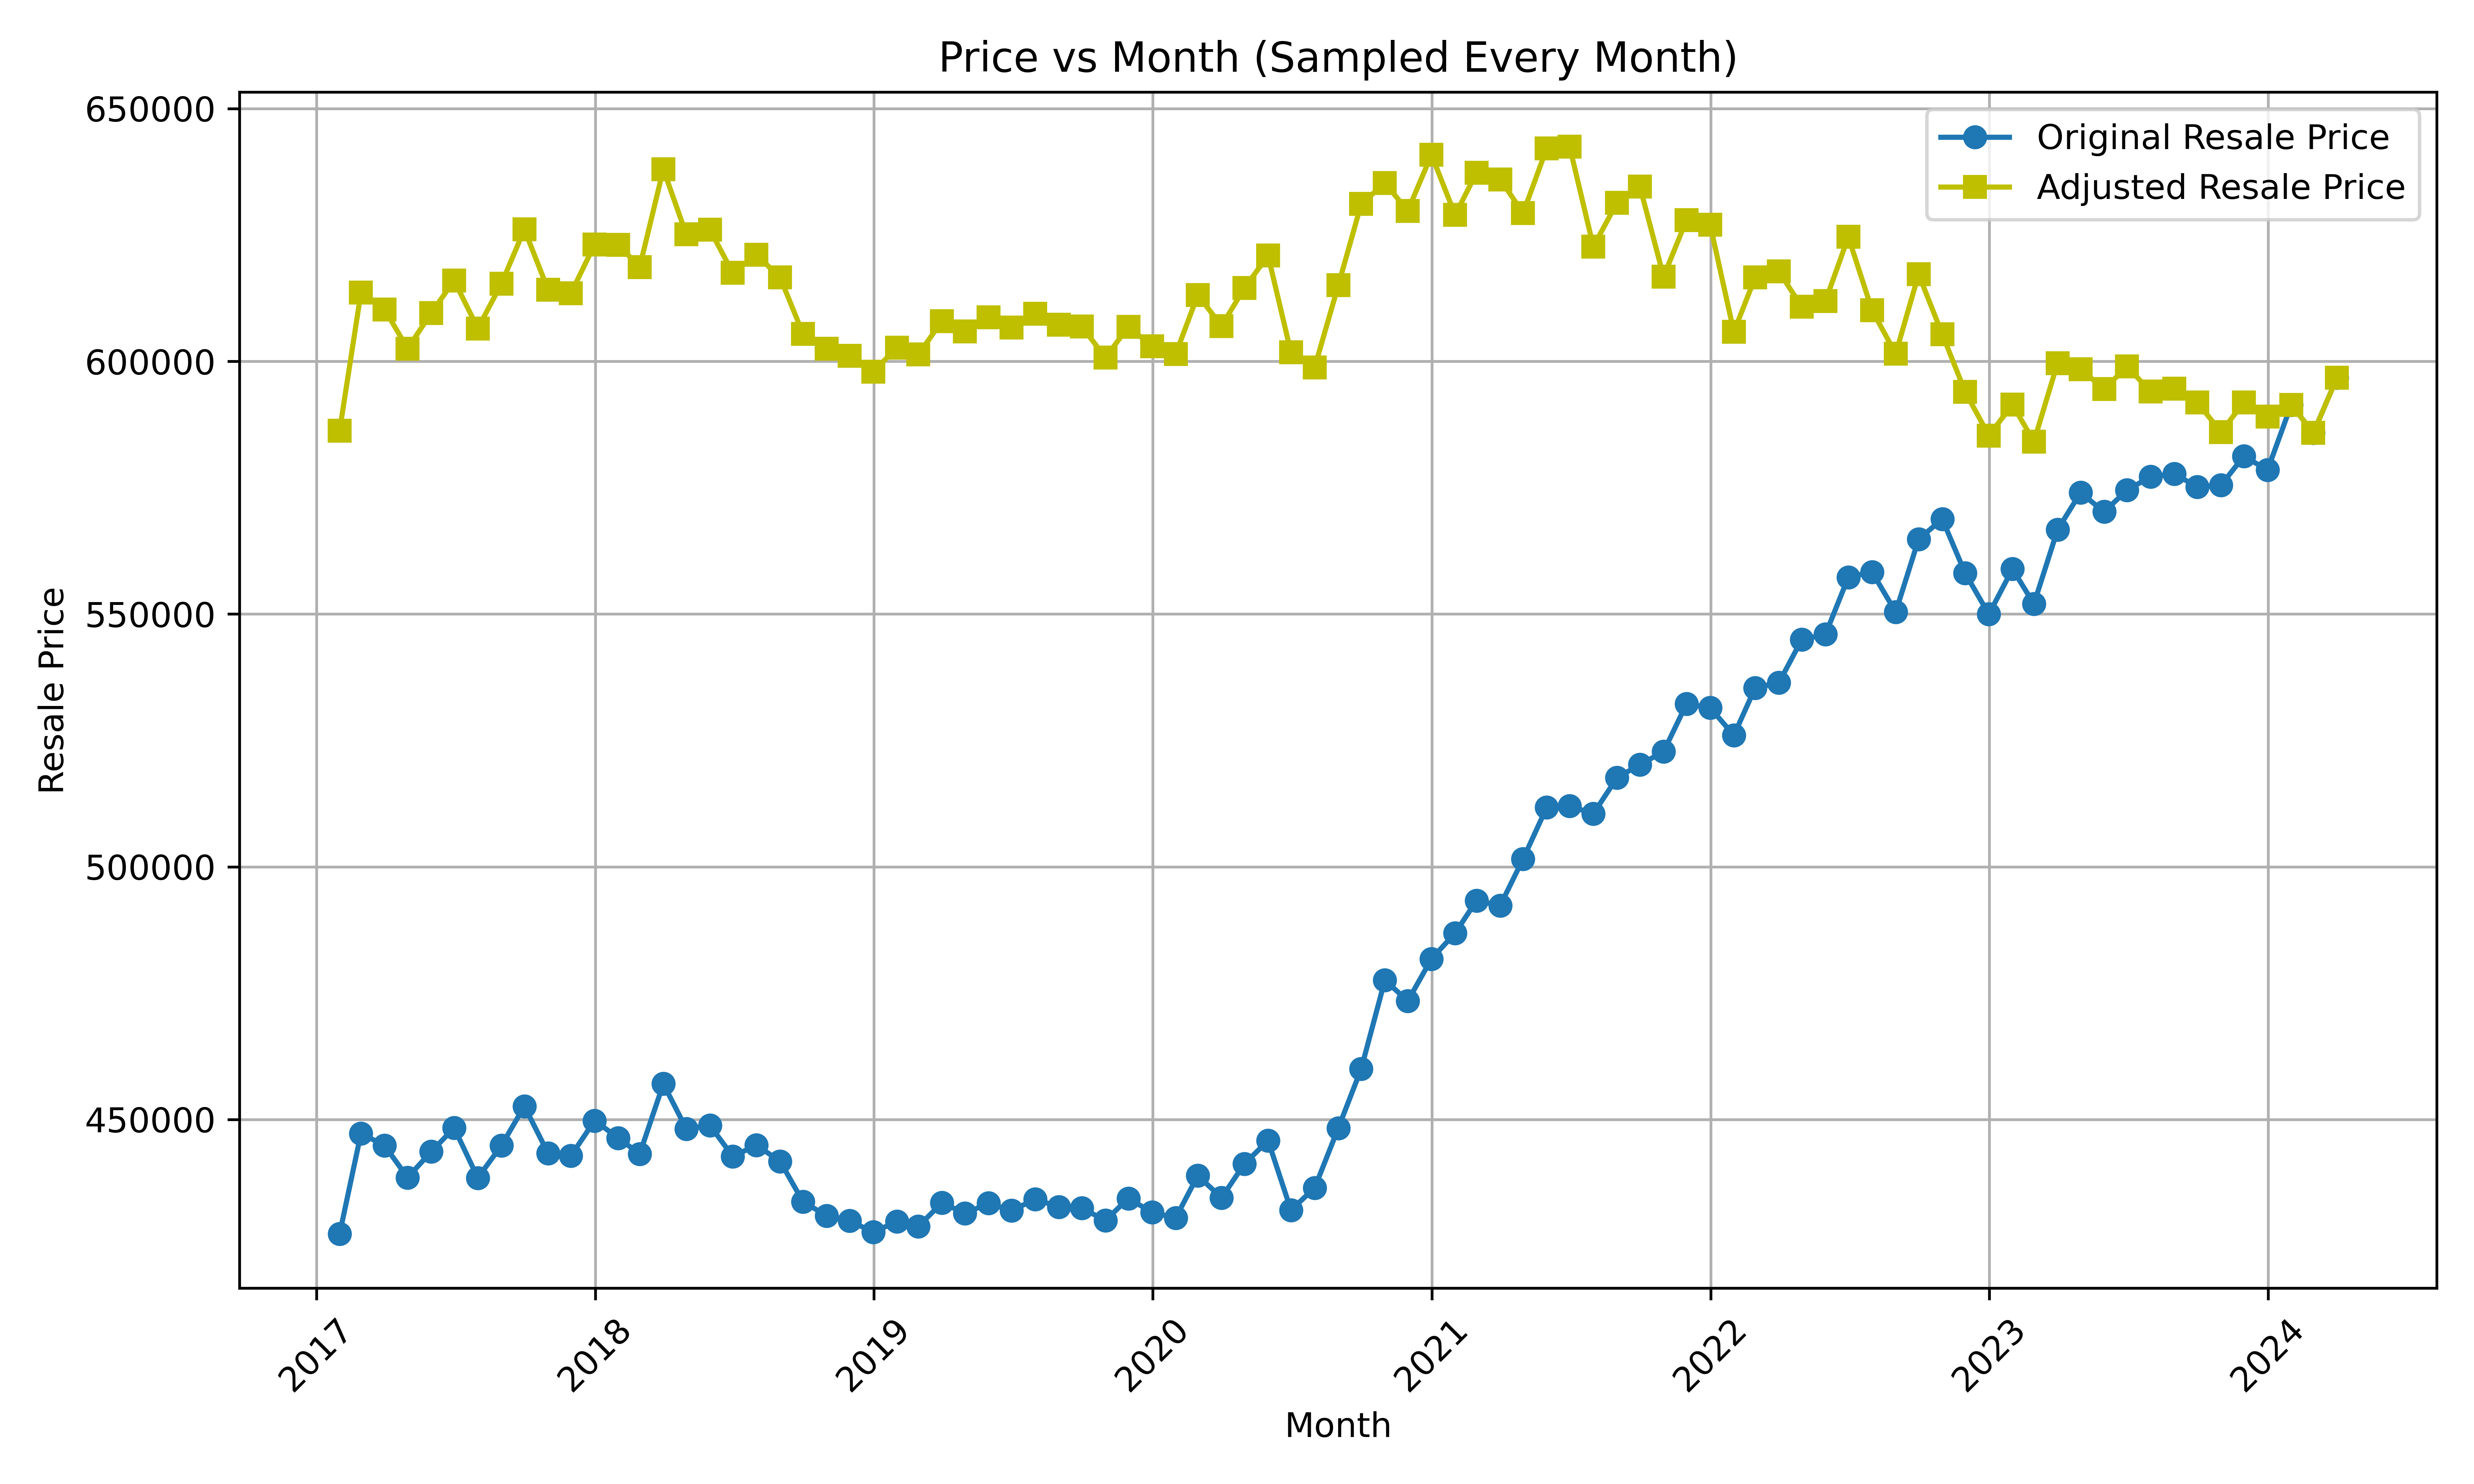
\includegraphics[width=0.75\textwidth]{imgs/adjusted_price.png}
\caption{Comparative illustration: Resale Price vs. Adjusted Price - Mitigating Inflationary Effects }\label{fig:priceinflation}
\end{figure}

Feature engineering ဆိုသည်မှာ မူလ dataset တွင် ပါ၀င်သည့် အချက်အလက်များကို မူတည်၍ အချက်အလက် အသစ်များ ဖန်တီးခြင်း၊ မူလ အချက်အလက်များကို machine learning မော်ဒယ် တည်ဆောက်ရာတွင် ပိုမို အဆင်ပြေစေရန် ပြုပြင်ခြင်းများကို ခေါ်သည်။ မူလ datasetတွင် တိုက်ခန်း၏ လက်ကျန်သက်တမ်း (\textit{\textbf{remaining lease}}) ကို ဖော်ပြရာ၌ ခုနှစ်နှင့်လ - ၂ ခုလုံးကို ဖော်ပြသည်။ အဆိုပါ အချက်အလက်ကို တွက်ချက်မှု ပြုလုပ်ရာတွင် လွယ်ကူစေရန်အတွက် စုစုပေါင်းလဖြင့် ဖော်ပြမည်။ ဥပမာ - သက်တမ်း ၄၁ နှစ် ၆ လ - ကျန်သည့် တိုက်၏ လက်ကျန်သက်တမ်းကို ဖော်ပြရာတွင် ၄၉၈ လ ဟု  လ အရည်အတွက်နှင့် ဖော်ပြသွားမည်။ 

အထက်ပါပုံတွင် တိုက်ခန်း၏ စျေးနှုန်းများကို လ အလိုက် နှိုင်းယှဥ်ကြည့်ရာ (အပြာရောင်လိုင်းဖြင့် ဖော်ပြထားသည်) တိုက်ခန်းများ၏ စျေးနှုန်းသည် အချိန်အလိုက် ပြောင်းလဲနေသည်ကို တွေ့ရမည်။ အထူးသဖြင့် ၂၀၂၁ နောက်ပိုင်း တွင် သိသိသာသာ စျေးနှုန်းများ ပြန်လည် မြင့်တက်လာသည်ကို တွေ့နိုင်သည်။ အဆိုပါ အချက်သည် အနာဂတ်တွင် ဖြစ်ပေါ်မည့် စျေးနှုန်းကို ခန့်မှန်းရာတွင် အသုံး၀င်သည့် အချက်ဖြစ်သော်လည်း တိုက်ခန်း၏ အခြားအချက်အလက်များဖြစ်သည့် အကျယ်အ၀န်း၊ တည်နေရာ စသည့် အချက်အလက်များကို မူတည်၍ စဥ်းစားရာတွင်မူ သတိထားရမည့် အချက် ဖြစ်လာသည်။ ဥပမာ -- ၂၀၂၃ တွင် ၅ သိန်း ၅ သောင်းနှင့် ရောင်းချခဲ့သည့် တိုက်ခန်းကို ၂၀၂၄ ခုနှစ် တွင် ရောင်းချမည်ဆိုပါက ၆ သိန်း နီးပါးဖြင့် ရောင်းချမည် ဖြစ်သည်။ သို့ဖြစ်ရာ တိုက်ခန်း၏ စျေးနှုန်းကို တွက်ချက်ရာတွင် မူလ ပေးထားသည့် စျေးနှုန်းအတိုင်း တိုက်ရိုက်တွက်ချက်ခြင်း မပြုဘဲ ၂၀၂၄ ခုနှစ်တွင် ဖြစ်ပေါ်မည့် ခန့်မှန်း စျေးနှုန်းကို မူတည်၍ စဥ်းစားသွားမည်။ ၂၀၂၄ ခုနှစ် ပထမ ၃ လ (ဇန်န၀ါရီမှ မတ်လ) အတွင်း ဖြစ်နိုင်သည့် စျေးနှုန်းကို သိရှိရန်အတွက်မူ Singapore အစိုးရမှ ထုတ်ပြန်ထားသည့် HDB resale price index ကို အသုံးပြု၍ ညှီမျှခြင်း \ref{eqn:adjusted_price}  တွင် ဖော်ပြထားသည့်အတိုင်း ခန့်မှန်းသွားမည် ဖြစ်သည်။ 

\subsubsection{Model Development: Build a Neural Network using Keras}
After data preprocessing, the clean dataset maintains its original size with 175,672 rows and now consists of 52 columns. The target variable is the \textit{\textbf{inflation-adjusted price}}, while the remaining 51 columns serve as features for training the neural network (deep learning) model. This section provides an explanation of each step in building the model. 

အထက်ပါ data preprocessing အဆင့်ဆင့်ကို ပြုလုပ်ပြီးနောက် dataset အသစ်တွင် အရောင်း စာရင်း အရေအတွက်မှာ မူလအတိုင်း တစ်သိန်း ခုနစ်သောင်း ငါးထောင် ခြောက်ရာ ခုနစ်ဆယ့် နှစ်ခု (၁၇၅,၆၇၂) ဖြစ်သော်လည်း column အရေအတွက်မှာမူ ၅၂ ခု အထိတိုးလာသည်။ inflation ကို ထည့်သွင်းစဥ်းစားထားသည့် စျေးနှုန်းကို Target အဖြစ်ထား၍ ခန့်မှန်းမည် ဖြစ်ပြီး ကျန် column ၅၁ ခု ကို Neural Network (deep learning model) ၏ input များ အဖြစ် အသုံးပြုမည်။ 

\begin{step} 
The project starts by importing the pandas library and loading a cleaned CSV file named \emph{\textbf{SGHDB2017-2024\_clean.csv}} into a Pandas DataFrame $df$. Then, the \emph{\textbf{adjusted\_price}} column, which represents the housing prices to be predicted, is extracted and stored in the variable $y$ and the remaining columns, which serve as features for the model, are stored in the variable $X$.

အဆင့် (၁) တွင် ဦးစွာ ပထမ  dataset အသစ် ကို Pandas DataFrame $df$ အဖြစ် သိမ်းဆည်းခြင်း ဖြစ်သည်။ ထို့နောက် အသုံးပြုမည့် Target ကို variable $y$ အဖြစ်လည်းကောင်း၊ ကျန် column များကို variable $X$ အဖြစ်လည်းကောင်း သိမ်းဆည်းမည်။ 

        \begin{lstlisting}
        # =========================================================================#
        import pandas as pd
        df = pd.read_csv('SGHDB2017-2024_clean.csv')
        y = df['adjusted_price'].values  
        X = df.drop(columns = 'adjusted_price')  
        # =========================================================================#
    \end{lstlisting}
\end{step}
\begin{remark}
    Ensure you have the necessary libraries installed. You can install them using pip if they are not already installed. For example: 
    \begin{lstlisting}
        pip install tensorflow pandas scikit-learn
    \end{lstlisting}
    သတိပြုရမည့် အချက်မှာ လိုအပ်သည့် library များကို  install ပြုလုပ်ရန် ဖြစ်သည်။ အကယ်၍ install မပြုလုပ်ရသေးပါက အထက်ပါ ကုဒ်ကို အသုံးပြု၍ install ပြုလုပ်ပေးရမည်။ 
\end{remark}

\begin{step}
This step prepares the data for building the machine learning model. 
\begin{itemize}
  \item The data is first split into training and testing sets, with 70\% of the data used for training (\(X_{\text{train}}\) and \(y_{\text{train}}\)) and 30\% for testing (\(X_{\text{test}}\) and \(y_{\text{test}}\)). The \texttt{random\_state=42} ensures reproducibility of the split.
  \item The continuous features are standardized using \texttt{StandardScaler}, which scales the data to have a mean of 0 and a standard deviation of 1. This transformation is applied separately to the training and testing sets to prevent data leakage. In this dataset, there are four continuous features: \texttt{flat\_type}, \texttt{floor\_area\_sqm}, \texttt{floor}, and \texttt{remaining\_lease\_months}.
  \item The scaled continuous features are combined with the binary features to form the final training (\(X_{\text{train}}\)) and testing (\(X_{\text{test}}\)) sets.
\end{itemize}

ဒုတိယ အဆင့်တွင် machine learning model တည်ဆောက်ရန် ဒေတာ အချက်အလက်များကို ပြင်ဆင်ရမည် ဖြစ်သည်။

ဦးစွာ ပထမ datasetကို training အတွက် ၇၀ ရာခိုင်နှုန်းကို အသုံးပြုပြီး ကျန် ၃၀ ရာခိုင်နှုန်းကို testing အတွက် ချန်ထားမည် ဖြစ်သည်။ ထို့နောက် continuous features များ ဖြစ်သည့် \texttt{flat\_type}၊ \texttt{floor\_area\_sqm}၊  \texttt{floor}, နှင့် \texttt{remaining\_lease\_months} များကို \texttt{StandardScaler} method ကို အသုံးပြု၍ range တစ်ခုအတွင်းရှိအောင် ပြုလုပ်ရမည်။ ထိုသို့ ပြုလုပ်ရာတွင် data leakage မဖြစ်စေရန် training နှင့် testing ဒေတာများကို သီးသန့်စီ ပြုလုပ်ရမည် ဖြစ်သည်။ 

\end{step}
\begin{lstlisting}
    # =========================================================================#
    import numpy as np
    from sklearn.preprocessing import StandardScaler
    from sklearn.model_selection import train_test_split
    # Step 2: Prepare the data
    X_train, X_test, y_train, y_test = train_test_split(X, y, test_size=0.3, random_state=42)

    # Standardize continuous features
    continuous_columns = ['flat_type', 'floor_area_sqm',  
                                   'floor', 'remaining_lease_months']
    binary_columns = df.columns.difference(continuous_columns 
                               + ['adjusted_price']).tolist()
    scaler = StandardScaler()
    X_train_continuous = scaler.fit_transform(X_train[continuous_columns])
    X_test_continuous = scaler.transform(X_test[continuous_columns])
    
    # Combine scaled continuous features and binary features
    X_train = np.hstack([X_train_continuous, X_train[binary_columns].values])
    X_test = np.hstack([X_test_continuous, X_test[binary_columns].values])
    # =========================================================================#
\end{lstlisting}  
\begin{step}
This step defines a function \texttt{create\_regression\_model} that constructs a feedforward neural network model for regression using TensorFlow's Keras API. 

တတိယ အဆင့်သည် TensorFlow ၏ Keras API ကို အသုံးပြု၍ neural network model တစ်ခု တည်ဆောက်ခြင်း ဖြစ်သည်။ ယခု model တွင် hidden layer - ၂ ခုသာ ပါ၀င်မည်ဖြစ်ပြီး ပထမ hidden layer တွင် neuron - ၃၂ ခု နှင့် ဒုတိယ hidden layer တွင် neuron -၁၆ ခု ကို အသုံးပြုမည်။ layer - ၂ ခုလုံးအတွက် ReLU activation function ကို အသုံးပြုထားသည်။ 

\begin{itemize}
    \item This function takes \texttt{input\_shape} as a parameter, representing the shape of the input data.
    \item Inside the function, a sequential model, as illustrated in Figure \ref{fig:mlp}, is created using \texttt{tf.keras.Sequential()}. 
    \item The model comprises an input layer, two hidden layers, and an output layer:
    \begin{itemize}
       \item The input layer serves as the initial receiver of input data, passing it to subsequent layers for processing.
       \item The first hidden layer is a fully connected (dense) layer with 32 units and ReLU activation function, as depicted in Figure \ref{fig:relu}.
       \item The second hidden layer is also fully connected, with 16 units and ReLU activation function.
       \item These hidden layers learn intricate patterns among the features.
       \item The output layer has a single unit, representing the regression prediction.
    \end{itemize}
    
    \item The code \texttt{model.compile(optimizer='adam', loss='mean\_squared\_error')} configures the neural network model. This project employs the \texttt{Adam} optimizer, an adaptive learning rate optimization algorithm. \texttt{Adam} adjusts the learning rate during training, facilitating faster convergence and improved performance. Additionally, \texttt{'mean\_squared\_error'} is used as the loss function, quantifying the difference between predicted and actual outputs during training.
\end{itemize}
\end{step}
\begin{lstlisting}
    # =========================================================================#
    import tensorflow as tf
    def create_regression_model(input_shape):
        model = tf.keras.Sequential([
            tf.keras.layers.InputLayer(shape=input_shape),        
            tf.keras.layers.Dense(32, activation='relu'),
            tf.keras.layers.Dense(16, activation='relu'),
            tf.keras.layers.Dense(1)
        ])    
        model.compile(optimizer='adam', loss='mean_squared_error')
    
        return model
        # =========================================================================#
\end{lstlisting}   
\begin{remark}
The size of hidden layers and the number of layers in a neural network are critical hyperparameters that influence the model's capacity, performance, and generalization ability. Finding the optimal configuration often involves a balance between model complexity and simplicity, guided by the specific characteristics of the dataset and the requirements of the task at hand. 

Hidden layer အရေအတွက်နှင့် neuron အရေအတွက်တို့မှာ neural network  တစ်ခုအတွက် အရေးကြီးသည့် hyperparameter များဖြစ်ပြီး dataset နှင့် ဖြေရှင်းမည့် ပြဿနာပေါ်တွင် မူတည်သည်။ 
\end{remark}

\begin{step}
The model is trained using the training data  (\(X_{\text{train}}\) and \(y_{\text{train}}\)). The training process runs for 10 epochs (Refer definition in Section \ref{def:epoch}) with a batch size of 32. 

အဆင့် (၄) တွင် training data များကို အသုံးပြု၍ အဆင့် (၃) တွင် တည်ဆောက်ခဲ့သည် neural network model ကို  train မည်ဖြစ်သည်။ ထိုသို့ train ရာတွင် ပြုလုပ်မည့် အကြိမ် အရေအတွက်ကို ၁၀ ဟု သတ်မှတ်ထားသည်။ ထို့အပြင် dataset ရှိ  data ပေါင်း တစ်သိန်းကျော်ကို တပြိုင်နက်ထဲ train ပြုလုပ်မည့် အစား တကြိမ်တွင် ဒေတာ (တိုက်ခန်းတစ်ခန်း၏ အရောင်းအ၀ယ် မှတ်တမ်း) - ၃၂ ခုကိုသာ အသုံးပြု၍  အကြိမ်ကြိမ် train ပြုလုပ်မည် ဖြစ်သည်။ ထိုသို့ ပြုလုပ်ခြင်းဖြင့် လိုအပ်သည့် memory နှင့် computational load  များကို လျော့ချနိုင်သည်။ 
    
\begin{lstlisting}
    # =========================================================================#
    model = create_regression_model(input_shape=[X_train.shape[1]])
    model.fit(X_train, y_train, epochs=10, batch_size=32, 
                    validation_data=(X_test, y_test))
    # =========================================================================#
\end{lstlisting}
\end{step}
\begin{remark}
Batch size refers to the number of training examples utilized in one iteration. Instead of using the entire dataset at once, training is divided into smaller batches. Using batch training allows for more efficient computation, as it reduces the memory requirements and computational load compared to processing the entire dataset at once.
\end{remark}

\begin{step}
In the last step, the model's performance is validated using the testing data (\(X_{\text{test}}\) and \(y_{\text{test}}\)) and saves the evaluation results to a CSV file.

နောက်ဆုံးအဆင့်တွင် model ၏ performance ကို testing ဒေတာများ အသုံးပြု၍ ဆန်းစစ်မည်။ 

\begin{lstlisting}
# Evaluate the model
from sklearn.metrics import mean_squared_error
from sklearn.metrics import mean_absolute_error, mean_absolute_percentage_error
from sklearn.metrics import r2_score

df_results = pd.DataFrame(columns=['Train', 'Test'])

y_pred = model.predict(X_train)
df_results.loc['Mean Squared Error', 'Train'] = mean_squared_error(y_train, y_pred)
df_results.loc['Mean Aboslute Error', 'Train'] = mean_absolute_error(y_train, y_pred)
df_results.loc['Mean Aboslute Percentage Error', 'Train'] = 
                        mean_absolute_percentage_error(y_train, y_pred)*100
df_results.loc['R2 score', 'Train'] = r2_score(y_train, y_pred)


y_pred = model.predict(X_test)
df_results.loc['Mean Squared Error', 'Test'] = mean_squared_error(y_test, y_pred)
df_results.loc['Mean Aboslute Error', 'Test'] = mean_absolute_error(y_test, y_pred)
df_results.loc['Mean Aboslute Percentage Error', 'Test'] = 
                        mean_absolute_percentage_error(y_test, y_pred)*100
df_results.loc['R2 score', 'Test'] = r2_score(y_test, y_pred)

df_results = df_results.round(2)
df_results.to_csv('model_evaluation.csv')
\end{lstlisting}
\end{step}

\subsubsection{Results and Discussion}
In this project, the model was trained without hyper-parameter tuning and subsequently evaluated on unseen test data to assess its efficacy. As illustrated in Table \ref{tab:results}, the model demonstrates robust predictive capability, with both the training and testing phases yielding results that closely align with actual values. 

The similarity in performance between the training and unseen data suggests that the model is not overfitting and is effectively generalizing to new instances. However, it's worth noting that an error of approximately SG\$65,000 may be deemed significant, particularly considering the average price of transactions in the training data, which is reported at SG\$611,563.8. This discrepancy represents roughly a 10\% deviation from the actual price, indicating room for further improvement in the model's precision.

ယခု သင်ခန်းစာတွင် ဖော်ပြထားသည့် model သည် hyper-parameter tuning  မပြုလုပ်ဘဲ တည်ဆောက်ထားသည့် model ဖြစ်သည်။  သို့သော် လက်ရှိ model၏ ရလဒ်မှာ သင့်တော် ကောင်းမွန်သည်ကို တွေ့ရသည်။ ခန့်မှန်း စျေးနှုန်းနှင့် မူလ စျေးနှုန်း၏ ပျမ်းမျှ ကွာခြားချက်သည် ခြောက်သောင်း ငါးထောင် ရှိပြီး တိုက်ခန်းများ၏ ပျမ်းမျှ ရောင်းစျေးနှုန်းနှင့် နှိုင်းယှဥ်ကြည့်ပါက ၁၀ ရာခိုင်နှုန်းလောက်သာ ကွာဟမှု ရှိသည်။ 

model ၏ hyper-parameter များဖြစ်သည့် hider layer များနှင့် neuron အရေအတွက်များကို တိုးမြှင့် အသုံးပြုမည်ဆိုပါက ပိုမိုကောင်းမွန်သည့် ရလဒ်များကို ရရှိနိုင်သည်။ 

\vspace{1em}

\begin{table}[htbp]
    \centering
    \caption{Model Evaluation Metrics}
    \label{tab:results}
    \begin{tabular}{l|r|r}
    \hline
    & \textbf{Train} & \textbf{Test} \\
    \hline
    Mean Squared Error & SG\$86,394.48 & SG\$86,284.83 \\
    Mean Absolute Error & SG\$65,017.51 & SG\$64,877.22 \\
    Mean Absolute Percentage Error & 10.82 \%& 10.82 \%\\
    R2 score & 82 \% & 82\% \\
    \hline
    \end{tabular}
\end{table}
\begin{remark}
The performance can be further enhanced by tuning the hyperparmeters, for instance, increasing the size of the hidden layers and depth of the neural network. 
\end{remark}
\newpage
\setcounter{stepcounter}{0}
\subsection{Multi-class Classification: Name Classification for Regional Identification} \label{sec:MMnames}
The objective of this project is to develop a machine learning model (neural network) specifically tailored to classify names to the corresponding states and regions within Myanmar. This model aims to address the challenges faced in demographic analysis and information extraction from news articles, where non-standardized writing of location names impedes accurate data interpretation.

အများသိကြသည့်အတိုင်း မြန်မာနိုင်ငံတွင် မူလက တိုင်းနှင့်ပြည်နယ် ၁၄ ခု ရှိခဲ့ပြီး ယခုအခါ နေပြည်တော် တိုးလာသည့်အတွက် ၁၅ ခု ရှိသည်။ ထို့အပြင် ရှမ်းကို ရှမ်း တောင်၊ ရှမ်းမြောက်နှင့် ရှမ်း ရှေ့ ဟူ၍ လည်းကောင်း၊ ပဲခူးကို ပဲခူအနောက်နှင့် ပဲခူး အရှေ့ဟု လည်းကောင်း ထပ်မံခွဲခြားထားရာ တိုင်းနှင့် ပြည်နယ် ၁၈ ခု ရှိသည်ကို ဆိုရမည်။ ဤ project ၏ ရည်ရွယ်ချက်မှာ နေရာတစ်ခု၏ အမည်ကို ပေးလိုက်သည်နှင့် မည်သည့် တိုင်းနှင့် ပြည်နယ်အတွင်း ရှိသည်ကို ခန့်မှန်းပေးရန် ဖြစ်သည်။ 

\subsubsection{Background}
In Myanmar, conducting social study research often involves collecting addresses from users, which can be challenging due to the lack of standardization in writing town and region names, particularly for smaller towns. Similarly, in news articles written by both local and international organizations, names are often written in non-standard ways, leading to inaccuracies in extracting location-based information. This project seeks to alleviate these challenges by automating the process of identifying the geographic origins associated with individual names.

မြန်မာ သတင်းအချက်အလက် စီမံခန့်ခွဲရေးအဖွဲ့ (MIMU)\cite{web:MIMU} ၏ ၏ ၂၀၁၉ ခုနှစ် ဒီဇင်ဘာလ စာရင်းအရ မြန်မာနိုင်ငံတွင် မြို့ပေါင်း ၄၆၉ မြို့နှင့် ကျေးရွာပေါင်း ၁၃,၅၉၀ ရှိသည်။ အဆိုပါ ကျေးရွာ အုပ်စုများ၏ အမည်များ နှင့် မြို့အမည်များကို စာလုံးပေါင်းဖော်ပြရာတွင် ဒေသအခေါ်အဝေါ်များနှင့် ကွဲလွဲမှုများ ရှိနေပါသည်။ ထို့အပြင် ထုတ်ပြန်ထားသည့် အမည်စာရင်းနှင့် ဒေသအခြေပြု သတင်းမီဒီယာများ၏ ဖော်ပြ ချက်များ အကြား ကွဲလွဲမှုများ ရှိနေပါသည်။ အဆိုပါကွဲလွဲမှုများကြောင့် လူမှုရေးနှင့် ဆိုင်သည့် သုတေသနေ လုပ်ငန်းများသည် နေရာ ဒေသအလိုက် အချက်အလက်များကို သုံးသပ်ရာတွင် တိကျမှု ရရှိနိုင်ရန် အခက်အခဲ များနှင့် ရင်ဆိုင် ကြုံတွေ့နေရသည်။ နေရာတစ်ခု၏ အမည်ကို ပေးလိုက်သည်နှင့် မည်သည့် တိုင်းနှင့် ပြည်နယ်အတွင်း ရှိသည်ကို အလွယ်တကူ ခန့်မှန်းပေးနိုင်မည့် Machine Learning Model တစ်ခု ကို တည်ဆောက်ထားခြင်းဖြင့် ပို၍ တိကျသည့် အချက်အလက်များကို သုံးသပ်နိုင်ရန် ရည်ရွယ်သည်။ 

\subsubsection{Dataset}
The initial datasets are obtained from the Myanmar Information Management Unit (MIMU) Resource Centre \cite{web:MIMU}, which offers comprehensive lists of names alongside their corresponding states and regions within Myanmar. The first dataset comprises 14,047 villages spread across 18 regions and states, while the second dataset includes 536 towns with their respective regions and states. These datasets serve as references for geographical information.

Additionally, supplementary data is collected from news articles, where variations in the spelling and formatting of town names are common. This dataset consists of 58,789 records spanning the same 18 regions and states. It's important to note that due to the nature of data collection from news articles, duplicate entries are present. Towns and regions are frequently mentioned in the articles, resulting in duplicated data instances.

Each dataset consists of two columns: 'state-region-names' and 'names of the location' (either villages or towns). Subsequently, these three datasets undergo comprehensive cleaning and merging processes to ensure coherence and consistency in the final combined dataset.

ဤ project တွင် အသုံးပြုမည့် dataset ကို မြန်မာ သတင်းအချက်အလက် စီမံခန့်ခွဲရေးအဖွဲ့ (MIMU) မှ ထုတ်နှုတ် ရယူထားခြင်း ဖြစ်သည်။ အဆိုပါ အဖွဲ့သည် မြန်မာနိုင်ငံရှိ ၀န်ကြီးဌာနအချို့နှင့် အဖွဲ့အစည်းများ၏ အချက်အလက်ကို စုစည်းတင်ပြထားသည့် ယုံကြည်စိတ်ချရသည့် အဖွဲ့အစည်းတစ်ခု ဖြစ်သည်။ ပထမ dataset တွင် ကျေးရွာပေါင်း  တစ်သောင်း လေးထာင် လေးဆယ့် ခုနစ် ခု ၏ အမည်များနှင့် အဆိုပါ မြို့ တည်ရှိသည့် တိုင်းနှင့်ပြည်နယ်၏ အမည်တို့ ပါ၀င်သည်။ ဒုတိယ dataset တွင်မူ မြို့ပေါင်း ၅၃၆ မြို့၏ အမည်များနှင့် သက်ဆိုင်ရာ တိုင်းနှင့်ပြည်နယ်၏ အမည်များ ပါ၀င်သည်။ ထို့အပြင် သတင်းခေါင်းစဥ်များမှ မြို့ရွာများ၏ အမည်များကို ထုတ်နှုတ်ရယူထားသည့် တတိယ dataset တွင် ငါးသောင်း ရှစ်ထောင် ခုနစ်ရာ ရှစ်ဆယ့်ကိုးခု ပါ၀င်သည်။ အထူးသတိပြုရမည့် အချက်မှာ ဤ တတိယ datasetသည် သတင်းများမှ အချက်အလက်များကို ထုတ်နှုတ် စုစည်းသည် ဖြစ်ရာ အချို့ မြို့များ၏ အမည်မှာ တစ်ကြိမ်မက ပါ၀င်နိုင်သည်။ 

dataset ၃ ခု လုံးတွင် column နှစ်ခု သာ ပါ၀င်ပြီး ပထမ column တွင် တိုင်းနှင့် ပြည်နယ်၏ အမည်များ ပါ၀င်သည်။ ဒုတိယ column တွင်မူ ကျေးရွာ(သို့မဟုတ်) မြို့၏ အမည်များ ပါ၀င်သည်။ 

\subsubsection{Data Preprocessing: Data Cleaning}
One of the major challenges in this project is name consistency, even for the names of the regions and states. For instance, the regions and states in the MIMU dataset are defined as "shan (south)," but in the news articles, they are usually defined as "shan-south." This inconsistency necessitates intensive data cleaning to ensure uniformity across datasets.

\begin{itemize}
  \item \textbf{Standardizing Column Names}: The column names of three datasets are standardized to ensure consistency. Specifically, the columns representing the names of regions and states are renamed to `SR\_Name' for uniformity across datasets.
  \item \textbf{Standardizing Naming Convention}:Fuzzy string matching techniques are employed to address variations in naming conventions between datasets. Specifically, the names in the news articles dataset are compared to the standardized names in the MIMU dataset, and the closest matches are identified and used to replace inconsistent names.
  \item \textbf{Removing Duplicates}: Duplicate rows in the news articles dataset are removed to enhance data quality and reduce redundancy.
  \item \textbf{Merging} The cleaned and standardized datasets are combined to form a comprehensive dataset (df\_mimu), consolidating information from both the MIMU dataset and news articles. This merged dataset encompasses 19,513 entries across 2 columns, enabling seamless progression to further analysis and modeling.
\end{itemize}

မြန်မာ သတင်းအချက်အလက် စီမံခန့်ခွဲရေးအဖွဲ့ (MIMU) မှ ရယူထားသည့် dataset တွင် ရှမ်း (တောင်)၊ ရှမ်း (မြောက်) - စသည်ဖြင့် တောင်နှင့် မြောက်ကို ကွင်းစ ကွင်းပိတ်နှင့် အသုံးပြု ဖော်ပြထားသော်လည်း သတင်းဌာနမှ ရယူထားသော ပြည်နည် အမည်များတွင်မူ ရှမ်း -တောင်၊  ရှမ်း -မြောက် စသည်ဖြင့် `-' ကို အသုံးပြု ထားသည်။ အဆိုပါ အမည် သတ်မှတ်ချက်များကို ကိုက်ညီစေရန် အတွက် Fuzzy string matching ကို အသုံးပြုသည်။ ထို့အပြင် သတင်းဌာနမှ ရယူထားသည့် dataset ထပ်နေသည့် မြို့အမည်၊ ကျေးရွာအမည်များကို ဖယ်ထုတ်သည်။ ထို့နောက် dataset ၃ ခု လုံးကို တစ်စုတည်းပေါင်းစည်းလိုက်ပြီး စုပေါင်း dataset တွင် record စုစုပေါင်း -- တစ်သောင်း ကိုးထောင် ငါးရာ တစ်ဆယ့်သုံးခုနှင့် column နှစ်ခု ပါ၀င်သည်။ 

\subsubsection{Data Preprocessing: Text Encoding (Vectorization)}

In this step, the text inputs from the 'name' column and the class labels from the 'SR\_Name' column are transformed into numerical representations. This transformation is necessary to convert the textual data into a format that can be processed by a neural network. 

\begin{itemize}
  \item Label encoding is applied on the `SR\_Name' column to map each unique stage/region name to a numerical value. Label encoding assigns a unique integer label to each unique category in the column.
  \item One-hot encoding is applied to the 'name' column because each name represents a specific location, and there is no ordinal relationship between the different names. This encoding method transforms categorical variables into binary vectors, where each unique category (name) is represented by a binary feature. This results in a sparse matrix with 13,003 binary columns, each representing a distinct name.
\end{itemize}

ဤ dataset တွင် ပါ၀င်သည့် အချက်အလက်များမှာ စာသားများဖြင့် ဖော်ြပ ထားသည် ဖြစ်ရာ ကိန်းဂဏန်းများ အဖြစ် ဦးစွာပြောင်းလဲမည်။ တိုင်းနှင့်ပြည်နယ်များ၏ အမည်များပါ၀င်သော `SR\_Name' column ကို Label encoding အသုံးပြု၍ ကိန်းဂဏန်းများအဖြစ် တိုက်ရိုက် ပြောင်းလဲမည်။ ဥပမာ -- ရှမ်း (တောင်) ကို ၁၅ ၊ ရခိုင်ကို ၁၂  ၊ ဧရာ၀တီကို သုည စသည်ဖြင့် သတ်မှတ်သည်။ ထို့နောက် ကျေးရွာအုပ်စုများနှင့် မြို့များ၏ အမည်ကို One-hot encoding နည်းစနစ်ကို အသုံးပြု၍ Binary Column များအဖြစ် ပြောင်းလဲမည်။ ဤ dataset တွင် ကျေးရွာအုပ်စုများနှင့် မြို့များ၏ အမည် စုစုပေါင်း တစ်သောင်း သုံးထောင် သုံးခု ပါ၀င်ရာ dataset ၏ record (row) တစ်ခုစီကို ($1 \times 13,003$) binary array များဖြင့် ဖော်ပြသွားမည်။ 

\subsubsection{Model Development: Build a Neural Network using Keras}
With the merged dataset containing 19,513 entries across 2 columns, the second column `name' of the location is used as an input feature and the first column `SR\_Name' is the class label (output) for the model. The section explains the steps for developing a neural network model using Keras for classifying the text inputs to 18 different regions and stages.  

%------step 1------
\begin{step} 
The first step in our data processing pipeline involves loading the data into a pandas DataFrame. This is accomplished using the pandas library, which is imported at the beginning of the script.

အဆင့် (၁) တွင် ဦးစွာ ပထမ  dataset ကို Pandas DataFrame $df$ အဖြစ် သိမ်းဆည်းခြင်း ဖြစ်သည်။ 

\begin{lstlisting}
# =========================================================================#
# Step 1: Load the data
import pandas as pd
df = pd.read_csv('./data/MMNames_clean.csv')
# =========================================================================#
\end{lstlisting}
\end{step}
\begin{remark}
    Ensure you have the necessary libraries installed. You can install them using pip if they are not already installed. For example: 
    \begin{lstlisting}
        pip install tensorflow pandas scikit-learn
    \end{lstlisting}
    သတိပြုရမည့် အချက်မှာ လိုအပ်သည့် library များကို  install ပြုလုပ်ရန် ဖြစ်သည်။ အကယ်၍ install မပြုလုပ်ရသေးပါက အထက်ပါ ကုဒ်ကို အသုံးပြု၍ install ပြုလုပ်ပေးရမည်။ 
\end{remark}
%------step 2-----
\begin{step}
This step prepares the data for building the machine learning model. This step involves preprocessing the data to get it ready for training a machine learning model. The code uses custom preprocessing functions in user-defined module `data\_preprocessing' and utilities from the sklearn library to achieve this.
\begin{itemize}
  \item The first three lines of the code below import the user-defined module `data\_preprocessing' and utilities from the sklearn library. 
  
  \item The code 'dp.preprocess\_category(df, 'SR\_Name')' preprocesses the \texttt{`SR\_Name'} column of the DataFrame df using label encoding. This method converts categorical values to numerical values, facilitating their use in machine learning algorithms.
  
  \item The code 'dp.preprocess\_category(df, 'name')'encodes the name column of the DataFrame df into a binary matrix representation using one-hot encoding. This technique enhances the model's ability to interpret and utilize categorical data effectively. 
      
  \item The preprocessed data is then split into training and testing sets, with 70\% of the data used for training (\(X_{\text{train}}\) and \(y_{\text{train}}\)) and 30\% for testing (\(X_{\text{test}}\) and \(y_{\text{test}}\)). The \texttt{random\_state=42} ensures reproducibility of the split.
\end{itemize}

ဒုတိယ အဆင့်တွင် machine learning model တည်ဆောက်ရန် ဒေတာ အချက်အလက်များကို ပြင်ဆင်ရမည် ဖြစ်သည်။ အောက်တွင် ပေးထားသော ကုဒ်၏ ပထမ ၃ ကြောင်းမှာ လိုအပ်သည့် module များကို import လုပ်ခြင်းဖြစ်သည်။ ထို့နောက် 'dp.preprocess\_category(df, 'SR\_Name')' ကုဒ်သည် `SR\_Name' column ကို Label encoding အသုံးပြု၍ ကိန်းဂဏန်းများအဖြစ် တိုက်ရိုက် ပြောင်းလဲခြင်းဖြစ်ပြီး 'dp.preprocess\_category(df, 'name')'သည်  ကျေးရွာအုပ်စုများနှင့် မြို့များ၏ အမည်ကို One-hot encoding နည်းစနစ်ကို အသုံးပြု၍ Binary Column များအဖြစ် ပြောင်းလဲပေးသည်။  ထို့နောက် datasetကို training အတွက် ၇၀ ရာခိုင်နှုန်းကို အသုံးပြုပြီး ကျန် ၃၀ ရာခိုင်နှုန်းကို testing အတွက် ချန်ထားမည် ဖြစ်သည်။ 
\end{step}
\begin{lstlisting}
# =========================================================================#
# Step 2: Prepare the data
import data_preprocessing as dp
from sklearn.preprocessing import StandardScaler
from sklearn.model_selection import train_test_split

df = dp.preprocess_category(df,'SR_Name')
df = dp.preprocess_onehot(df,'name')

y = df['SR_Name'].values 
X = df.drop(columns=['SR_Name']).values

X_train, X_test, y_train, y_test = train_test_split(X, y, test_size=0.3, random_state=42)
print(X_train.shape, X_test.shape)
# =========================================================================#
\end{lstlisting}
%-- step 3---
\begin{step}
This step defines a function \texttt{create\_regression\_model} that constructs a feedforward neural network model for classification using TensorFlow's Keras API. 

တတိယ အဆင့်သည် TensorFlow ၏ Keras API ကို အသုံးပြု၍ neural network model တစ်ခု တည်ဆောက်ခြင်း ဖြစ်သည်။ ယခု model တွင် hidden layer - ၂ ခုသာ ပါ၀င်မည်ဖြစ်ပြီး ပထမ hidden layer တွင် neuron - ၃၂ ခု နှင့် ဒုတိယ hidden layer တွင် neuron -၁၆ ခု ကို အသုံးပြုမည်။ layer - ၂ ခုလုံးအတွက် ReLU activation function ကို အသုံးပြုထားသည်။ 

\begin{itemize}
    \item This function takes \texttt{input\_shape} and \texttt{num\_classes} as parameters, representing the shape of the input data and the number of classes.
    \item The model comprises an input layer, two hidden layers, and an output layer:
    \begin{itemize}
       \item The input layer serves as the initial receiver of input data, passing it to subsequent layers for processing.
       \item The first hidden layer is a fully connected (dense) layer with 32 units and \texttt{ReLU} activation function, as depicted in Figure \ref{fig:relu}.
       \item The second hidden layer is also fully connected, with 16 units and \texttt{ReLU} activation function.
       \item These hidden layers learn intricate patterns among the features.
       \item The output layer has a single unit, representing the classification prediction. The \texttt{`softmax'} activation function is used in the output layer.
    \end{itemize}
    
    \item The code \texttt{model.compile(optimizer='adam', loss='sparse\_categorical\_crossentropy', metrics=['accuracy'])} configures the neural network model. 
    \item This project employs the \texttt{Adam} optimizer, an adaptive learning rate optimization algorithm. \texttt{Adam} adjusts the learning rate during training, facilitating faster convergence and improved performance. 
    \item The loss function \texttt{'sparse\_categorical\_crossentropy'}loss function is utilized, which calculates the cross-entropy loss between the predicted probabilities and the true labels. This loss function is suitable for multi-class classification tasks where the target labels are integers.
    \item The \texttt{`accuracy'} metric is selected to evaluate the model's performance. It measures the proportion of correctly classified samples out of the total number of samples, providing a straightforward assessment of the model's predictive accuracy.
\end{itemize}
\end{step}

\begin{lstlisting}
# =========================================================================#
import tensorflow as tf

def create_classification_model(input_shape, num_classes, params={}):
    model = tf.keras.Sequential([
        tf.keras.layers.InputLayer(shape=input_shape),
        tf.keras.layers.Dense(32, activation='relu'),
        tf.keras.layers.Dense(16, activation='relu'),
        tf.keras.layers.Dense(num_classes, activation='softmax')
    ])

    model.compile(optimizer='adam', 
                loss='sparse_categorical_crossentropy', metrics=['accuracy'])
    
    return model
     # =========================================================================#
\end{lstlisting}   
\begin{remark}
The size of hidden layers and the number of layers in a neural network are critical hyperparameters that influence the model's capacity, performance, and generalization ability. Finding the optimal configuration often involves a balance between model complexity and simplicity, guided by the specific characteristics of the dataset and the requirements of the task at hand. 

Hidden layer အရေအတွက်နှင့် neuron အရေအတွက်တို့မှာ neural network  တစ်ခုအတွက် အရေးကြီးသည့် hyperparameter များဖြစ်ပြီး dataset နှင့် ဖြေရှင်းမည့် ပြဿနာပေါ်တွင် မူတည်သည်။ 

\end{remark}
% step 4 ----
\begin{step}
The model is trained using the training data  (\(X_{\text{train}}\) and \(y_{\text{train}}\)). The training process runs for 10 epochs (Refer definition in Section \ref{def:epoch}) with a batch size of 32. 

အဆင့် (၄) တွင် training data များကို အသုံးပြု၍ အဆင့် (၃) တွင် တည်ဆောက်ခဲ့သည် neural network model ကို  train မည်ဖြစ်သည်။ ထိုသို့ train ရာတွင် ပြုလုပ်မည့် အကြိမ် အရေအတွက်ကို ၅၀ ဟု သတ်မှတ်ထားသည်။ ထို့အပြင် dataset ရှိ  data ပေါင်း တစ်သိန်းကျော်ကို တပြိုင်နက်ထဲ train ပြုလုပ်မည့် အစား တကြိမ်တွင် ဒေတာ - ၃၂ ခုကိုသာ အသုံးပြု၍  အကြိမ်ကြိမ် train ပြုလုပ်မည် ဖြစ်သည်။ ထိုသို့ ပြုလုပ်ခြင်းဖြင့် လိုအပ်သည့် memory နှင့် computational load  များကို လျော့ချနိုင်သည်။ 
    
\begin{lstlisting}
    # =========================================================================#
    model = create_classification_model(input_shape=[X_train.shape[1]],
                num_classes=len(df['SR_Name'].unique()), )
    history = model.fit(X_train, y_train, epochs=50, batch_size=32, 
                validation_data=(X_test, y_test), verbose=0)
    # =========================================================================#
\end{lstlisting}
\end{step}
\begin{remark}
Batch size refers to the number of training examples utilized in one iteration. Instead of using the entire dataset at once, training is divided into smaller batches. Using batch training allows for more efficient computation, as it reduces the memory requirements and computational load compared to processing the entire dataset at once.
\end{remark}

% ----step 5 ----

\begin{step}
In the last step, the model's performance is validated using the testing data (\(X_{\text{test}}\) and \(y_{\text{test}}\)) and saves the evaluation results to a CSV file. In this step, the \texttt{`classification\_report'} function from scikit-learn is used to generate a classification report for the actual test labels (\texttt{y\_test}) and the predicted labels (\texttt{y\_pred}).

နောက်ဆုံးအဆင့်တွင် model ၏ performance ကို testing ဒေတာများ အသုံးပြု၍ ဆန်းစစ်မည်။ 

\begin{lstlisting}
# Step 5: Evaluate the model

from sklearn.metrics import classification_report

y_pred = model.predict(X_test, batch_size=32, verbose=0)
y_pred = y_pred.argmax(axis=1)
report = classification_report(y_test, y_pred, output_dict=True)
report_df = pd.DataFrame(report).transpose()
report_df.to_csv('./data/cls_report_test.csv', index=False)
print(report_df)
y_pred = model.predict(X_train, batch_size=32, verbose=0)
y_pred = y_pred.argmax(axis=1)
report = classification_report(y_train, y_pred, output_dict=True)
report_df = pd.DataFrame(report).transpose()
report_df.to_csv('./data/cls_report_train.csv', index=False)

\end{lstlisting}
\end{step}

\subsubsection{Results and Discussion}
\begin{table}[htbp]
    \centering
    \caption{Model Evaluation Metrics}
    \label{tab:P2results}
    \begin{tabular}{l|r|r}
    \hline
    & \textbf{Train} & \textbf{Test} \\
    \hline
    Accuracy                            & 86\% & 28\% \\
    weighted average Precision & 87\% & 45\% \\
    weighted average Recall      & 86\% & 28\%\\
    \hline
    \end{tabular}
\end{table}

In the results presented above (Ref. Table \ref{tab:P2results}), it's evident that while the model attained an accuracy of 86\% on the training data, it only achieved 28\% on the test data. Similarly, the model demonstrated weighted average precision and recall rates of 87\% and 86\% on the training set, but notably dropped to 45\% and 28\% on the test set. These findings indicate that the developed neural network model, a fully connected multi-layer perceptron, isn't well-suited for this particular problem. Its overfitting can be attributed to its inability to capture sequential patterns and inherent relationships within textual data, such as location names. Such limitations often lead to poor generalization to new data, particularly when dealing with high-dimensional sparse datasets like one-hot encoded vectors.

This is where more advanced models, such as Recurrent Neural Networks (RNNs), come into play. RNNs are designed to recognize sequential patterns and dependencies in data by maintaining a hidden state that captures information from previous time steps. This makes RNNs particularly effective for tasks involving sequential data, such as natural language processing, where understanding the order and context of words (or characters) is crucial. 

%However, in this particular problem, a simpler model like Bernoulli Naive Bayes provides good performance, with an accuracy score of 0.78 for the testing set and 0.86 for the training set. This demonstrates that while neural networks are powerful, they might not always be necessary or the best choice for every classification problem.

In the next chapter, we will delve into the advanced deep learning models, particularly one particular section focusing on Recurrent Neural Networks (RNNs). We will explore their design principles, operational mechanisms, and why they are better suited for handling sequential data in tasks like sentiment analysis. 

အထက်ပါ ဇယားတွင် ဖော်ပြထားသည့် ရလဒ်များကို သုံးသပ်ကြည့်မည်ဆိုပါက ယခု သင်ခန်းစာတွင် တင်ပြထားသည့် neural network model (fully connected multi-layer perceptron) သည် အမည်များကို မှန်မှန်ကန်ကန် ခွဲခြားပေးနိုင်ခြင်း မရှိသည်ကို တွေ့ရသည်။ train ပြုလုပ်ထားသည့် data အတွက် ၈၆ ရာခိုင်နှုန်းလောက်ထိ ကောင်းမွန် တိကျသည့် ရလဒ်များကို ထုတ်ပေးနိုင်သော်လည်း အသစ် data များအတွက်မူ ၄င် model ၏ ရလဒ်မှာ ၅၀ ရာခိုင်နှုန်းအောက် ကျဆင်းသွားသည်။ Text data များကို အမျိုးအစား ခွဲခြားကြရာတွင် အများဆုံး အသုံးပြုသည့်  model မှာ  Recurrent Neural Networks (RNNs) ဖြစ်သည်။ အထူးသဖြင့် စကားလုံး တစ်လုံးမက ပါ၀င်သည့် စာကြောင်းများကို အမျိုးအစားခွဲခြားသည့် sentiment analysis ကဲ့ သို့ ပြဿနာများတွင် RNN ၏ စွမ်းဆောင်ရည်မှာ ပိုမိုကောင်းမွန်ကြောင်း သုတေသနပညာရှင်များက သက်သေပြခဲ့ပြီး ဖြစ်သည်။ 

%သို့သော် စကားလုံး တစ်လုံး ၊ နှစ်လုံးသာ ပါ၀င်သည့် ယခု ပြဿနာတွင်မူ ရိုးရှင်းလွယ်ကူသည့် Bernoulli Naive Bayes machine learning model ကို အသုံးပြုခြင်းဖြင့် ပို၍ ကောင်းမွန်သည့် ရလဒ်များ ရရှိသည်ကို တွေ့ရသည်။ neural networks (သို့မဟုတ်) deep learning model များသည် ယေဘူယျအားဖြင့် ပိုမိုကောင်းမွန်သည့် ရလဒ်များကို ပေးနိုင်သည်ဟု ဆိုသော်လည်း ပြဿနာတိုင်းအတွက် မဟုတ်သည်ကို သတိပြုသင့်သည်။  

နောက် အခန်းတွင် RNN အပါအ၀င် advanced deep learning model များကို ဆွေးနွေးသွားမည်။ 

\newpage

\section{Chapter-End Exercises}\label{sec:exercises}

This section provides chapter-end exercises aimed at reinforcing learning and assessing comprehension of the foundation of the neural network, activation function, forward propagation and backward propagation. Readers are encouraged to attempt these exercises independently prior to checking solutions.

\begin{question}
You have a neural network model with one hidden layer, as shown in Figure \ref{fig:Ex2-1}. The input data point has two features: $x_1=1$ and $x_2 = 1$. The ReLU activation function is used in the hidden layer, resulting in: $h_1 = 6$ and $h_2=0$ for the hidden layer outputs. The weights on the edges connecting the hidden and output layer are -1 and 1, respectively. What prediction ($y$) would this model make on this data point? Assume that the output layer uses the sigmoid function.
\end{question} 

\vspace{0.5em}
\begin{figure}[h]%
\centering
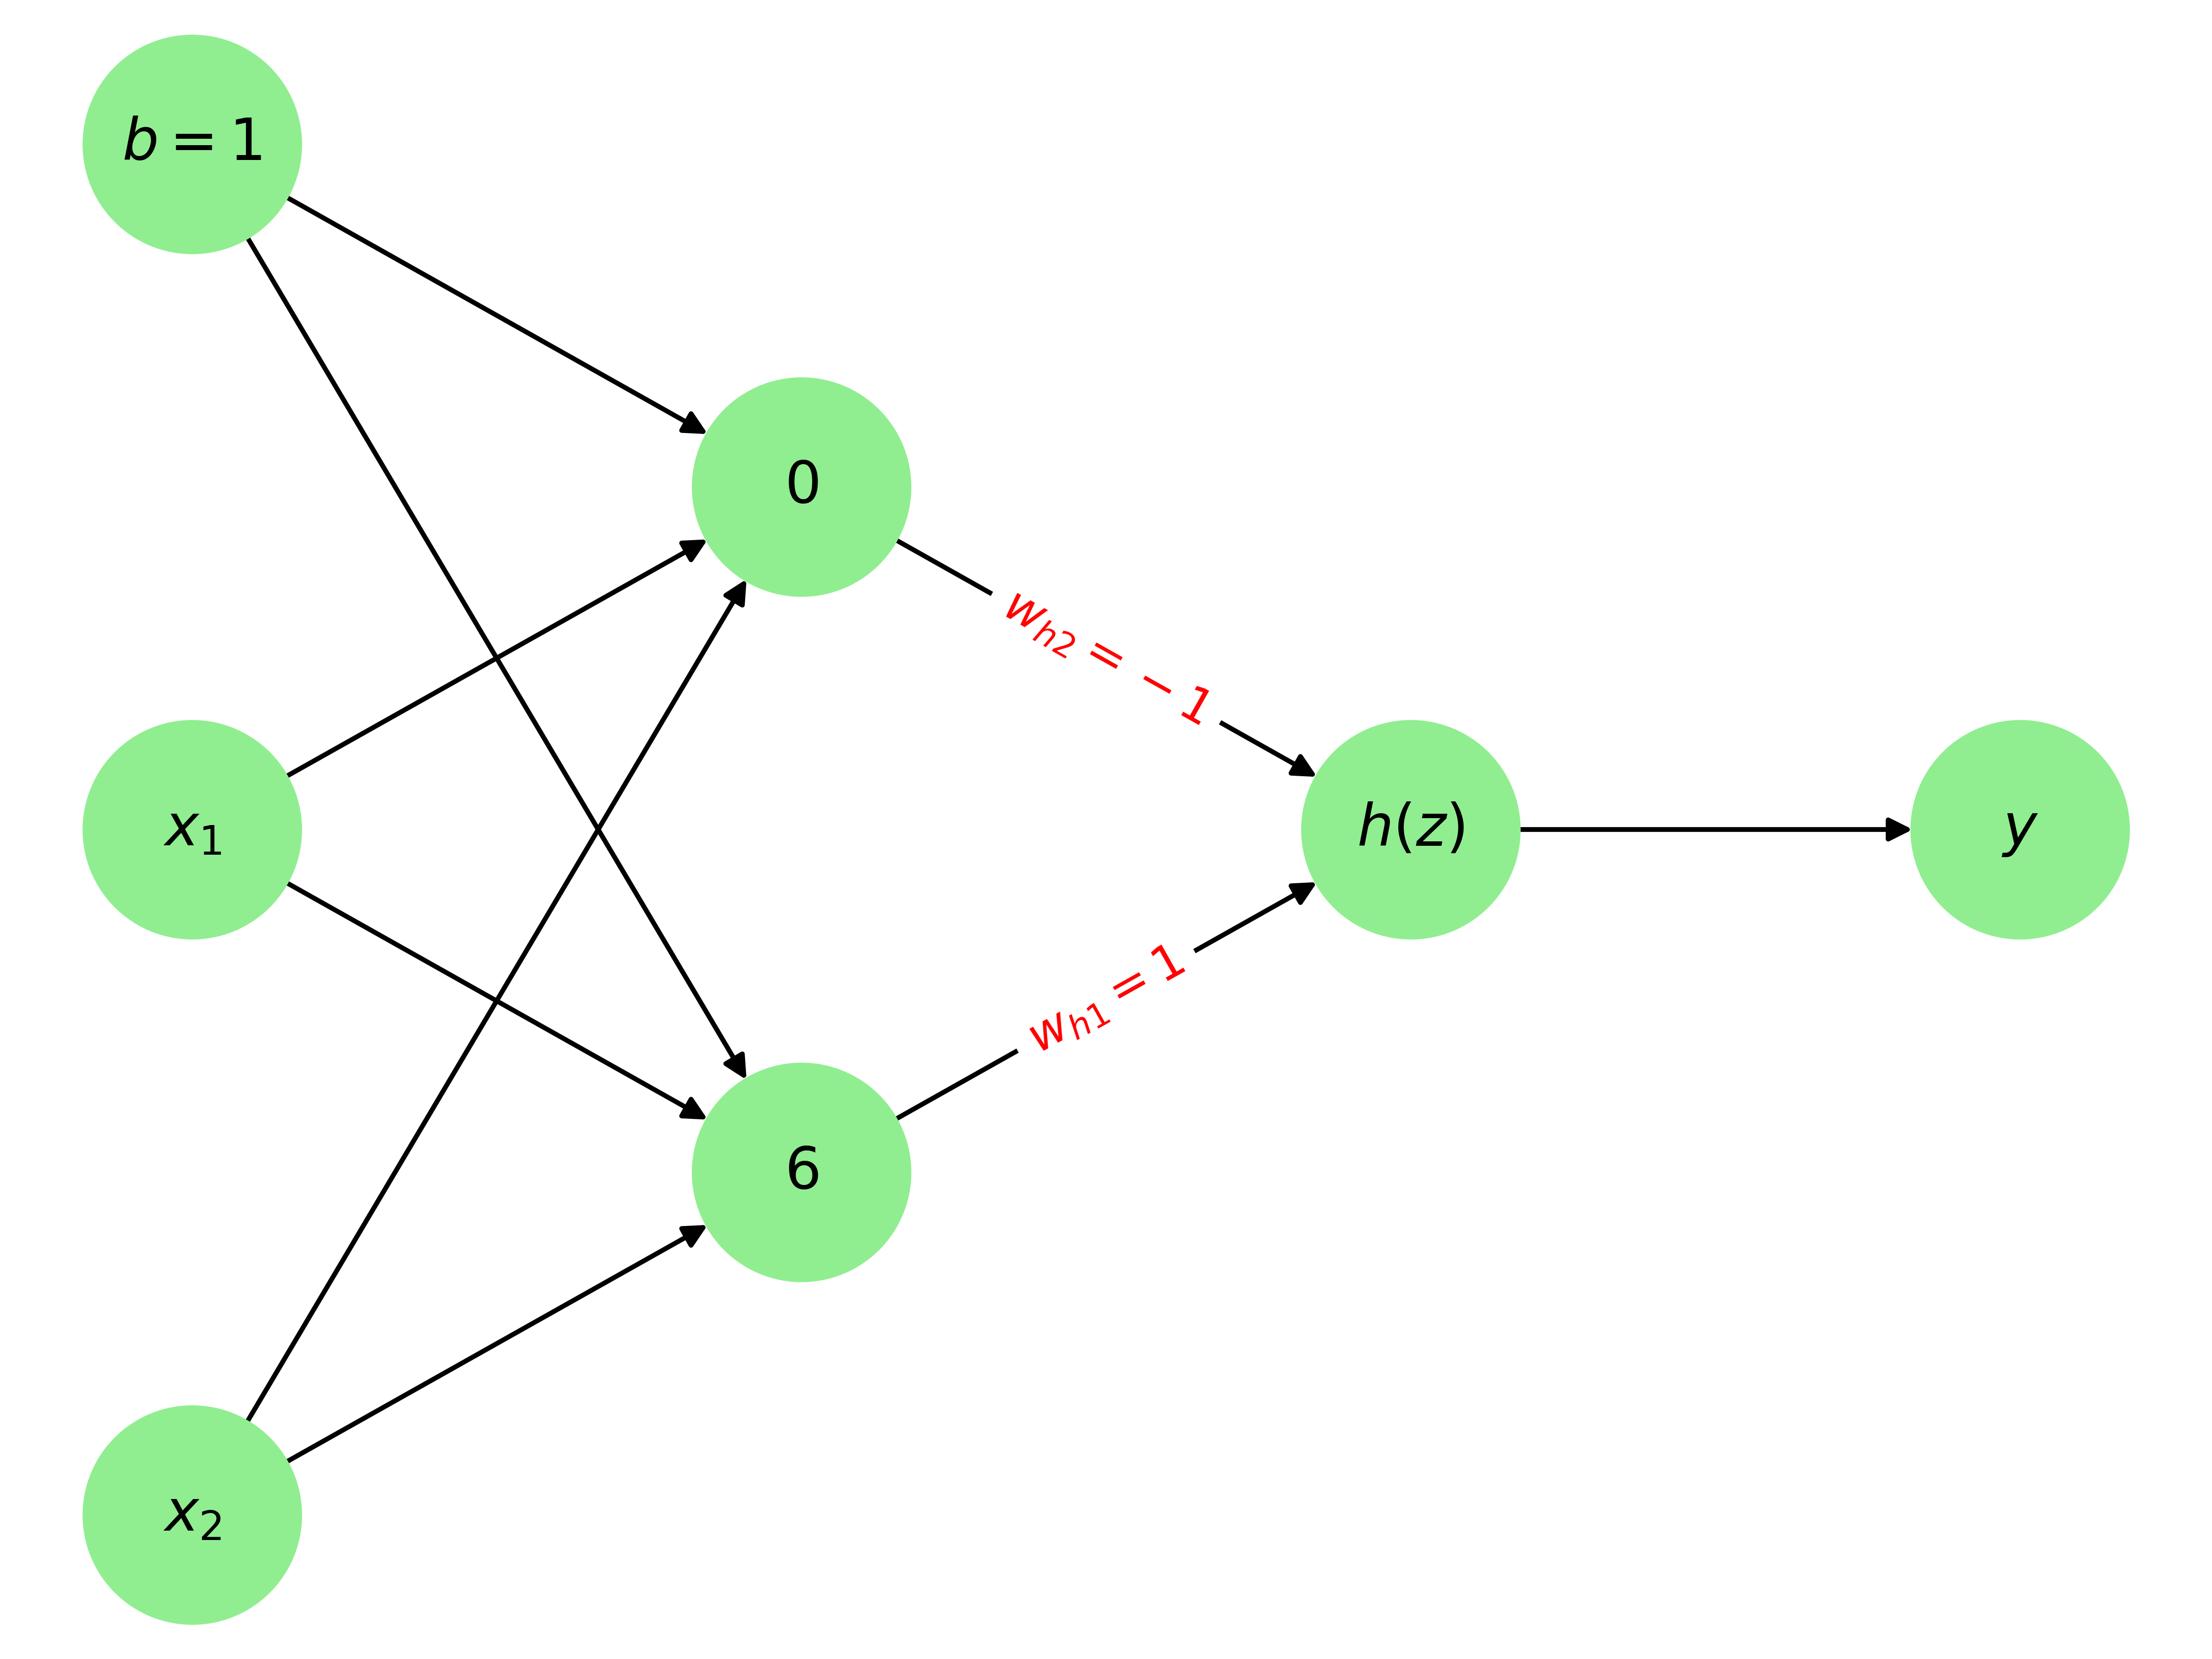
\includegraphics[width=0.675\textwidth]{imgs/chap2_ex1.png}
\caption{Forward Propagation in a NN with two hidden layers}\label{fig:Ex2-1}
\end{figure}

\begin{answer}
The weighted sum of the inputs to the output layer can be calculated as: 
\begin{equation}\label{eq:ex1}
  z = \omega_{h1}*h_1 + \omega_{h2}*h_2 = (1)*6 + (-1)*0 = 6
\end{equation} Then, applying the sigmoid activation function: the value of
\begin{equation}\label{eq:ex1}
  y = \frac{1}{1+\exp{(-6)}} = 0.997
\end{equation}
\end{answer}

\begin{question}
How are the weights that determine the features/interactions in Neural Networks created? 
\begin{tasks}(3) % Two-column tasks
    \task Define by the programmer. 
    \task Network learn during the training process. 
    \task Weights are defined randomly. 
\end{tasks}
\end{question} 

\begin{answer}
\textbf{Explanation}: In neural networks, the weights that determine the features and interactions are learned from the training data. During training, the network adjusts the weights iteratively through optimization algorithms such as gradient descent to minimize the difference between the predicted outputs and the actual outputs.
\end{answer}

\begin{question}
Which layers of a model capture more complex or "higher level" interactions?
\begin{tasks}(3) 
    \task Initial layers
    \task Deeper layers
    \task All Layers
\end{tasks}
\end{question} 

\begin{answer}
\textbf{Explanation}: In neural networks, deeper layers, in particular, tend to capture more abstract and complex features as they build upon the representations learned by earlier layers.
\end{answer}


\begin{question}
While training a neural network, what parameter is adjusted? 
\begin{tasks}(3) 
    \task The weights
    \task The numbers of nodes (units)
    \task The numbers of hidden layers 
\end{tasks}
\end{question} 

\begin{answer}
\textbf{Explanation}: During the training process, the weights of the connections between neurons are adjusted iteratively through optimization algorithms such as gradient descent. This adjustment of weights allows the neural network to learn from the input data and improve its performance on the task it is trained for.
\end{answer}

\begin{question}
What activation function is commonly used in the hidden layers of a neural network to introduce non-linearity?
\begin{tasks}(3)
\task Sigmoid
\task ReLU
\task Tanh
\end{tasks}
\end{question}

\begin{answer}
\textbf{Explanation}: In neural networks, the activation function in the hidden layers introduces non-linearity to the model, enabling it to learn complex patterns and relationships in the data. While all the provided activation functions introduce non-linearity, the Rectified Linear Unit (ReLU) is commonly used in the hidden layers due to its simplicity and effectiveness. ReLU replaces all negative values with zero, effectively making the activation function linear for positive values and zero for negative values.
\end{answer}

\begin{question}
In neural networks, which activation function is commonly used for multi-class classification tasks?
\begin{tasks}(2)
\task Softmax
\task Sigmoid
\end{tasks}
\end{question}

\begin{answer}
\textbf{Explanation}: Softmax activation function is typically used in the output layer of neural networks for multi-class classification tasks, where it normalizes the output into a probability distribution over multiple classes. Sigmoid activation function, on the other hand, is commonly used for binary classification tasks, where it squashes the output to a range between 0 and 1, representing the probability of the positive class.
\end{answer}

\begin{question}
What is the primary function of the Sequential model in the Keras library?
\begin{enumerate}[a]
\item To define the architecture of convolutional layers
\item To create a linear stack of layers for building neural networks
\item To perform data augmentation during training
\end{enumerate}
\end{question}

\begin{question}
What is the purpose of the compile method in Keras?
\begin{enumerate}[a]
\item To configure the learning process by specifying the optimizer, loss function, and evaluation metrics
\item To initialize the weights of the neural network layers
\item To preprocess the input data before training
\end{enumerate}
\end{question}

\begin{question}
How many hidden layers are there in the classification model discussed in Section \ref{sec:SGHDB}?
\begin{enumerate}[a]
\item One
\item Two
\item Three
\end{enumerate}
\end{question}

%\begin{question}
%How many hidden layers are there in the classification model discussed in Section \ref{sec:MMnames}?
%\begin{enumerate}[a]
%\item One
%\item Two
%\item Three
%\end{enumerate}
%\end{question}

\begin{question}
Which Keras module is commonly used for adding a layer?
\begin{enumerate}[a]
\item keras.preprocessing
\item keras.layers
\item keras.optimizers
\end{enumerate}
\end{question} 